\documentclass[12pt]{article}

\usepackage{graphicx}
\usepackage{float}
\usepackage{sbc-template}

\usepackage{graphicx,url}

\usepackage[brazil]{babel}   
\usepackage[utf8]{inputenc}  
\usepackage{pdflscape}
\usepackage{booktabs}
\usepackage{tabularx}
\usepackage{amsmath}
\sloppy

\title{Da Extração de Características à Combinação de Classificadores: Uma Análise Supervisionada de Imagens de Cães e Gatos}

\author{Gil César Faria\inst{1}}


\address{Instituto Metrópole Digital
  \\
  Universidade Federal do Rio Grande do Norte (IMD/UFRN)
  \email{gilcesarf@gmail.com}
}

\begin{document} 
\pagestyle{plain}

\maketitle

\begin{abstract}
This work applies \textit{supervised machine learning} techniques to the problem of \textit{binary classification of dog and cat images}. The data set contains 800 images, evenly divided between 400 dogs and 400 cats, with variations in lighting, focus, and background. The \textit{Histogram of Oriented Gradients} (HOG) and \textit{Local Binary Pattern} (LBP) were used for feature extraction. The classifiers applied were \textit{k-Nearest Neighbors}, Decision Tree, \textit{Naive Bayes}, and \textit{Multilayer Perceptron}, along with ensemble methods such as \textit{Bagging}, \textit{Random Forest}, \textit{Voting}, and \textit{Stacking}. The comparative analysis of the methods was conducted using the non-parametric statistical tests \textit{Friedman} and \textit{Nemenyi}.
\end{abstract}
     
\begin{resumo} 
Este trabalho aplica técnicas de \textit{aprendizado de máquina supervisionado} ao problema de \textit{classificação binária de imagens de cães e gatos}. O conjunto de dados contém 800 imagens, divididas igualmente entre 400 de cães e 400 de gatos, com variações de iluminação, foco e fundo. Foram utilizados os descritores \textit{Histogram of Oriented Gradients} (HOG) e \textit{Local Binary Pattern} (LBP) para extração de características. Os classificadores aplicados foram \textit{k-Nearest Neighbors}, Árvore de Decisão, \textit{Naive Bayes} e \textit{Rede Neural Multicamadas}, além dos comitês \textit{Bagging}, \textit{Random Forest}, \textit{Voting} e \textit{Stacking}. A análise comparativa dos métodos foi realizada por meio dos testes estatísticos de \textit{Friedman} e \textit{Nemenyi}.
\end{resumo}
\newpage
\section{Introdução}

O \textit{aprendizado de máquina supervisionado} reúne técnicas destinadas a identificar padrões em dados rotulados, permitindo a construção de modelos capazes de classificar novas instâncias com base em exemplos previamente conhecidos. Entre suas aplicações mais comuns está a tarefa de classificação, na qual o objetivo é distinguir categorias a partir de atributos derivados dos dados de entrada.

Neste trabalho, essas técnicas são aplicadas ao problema de \textit{classificação binária de imagens de cães e gatos}, com o intuito de analisar o comportamento de diferentes algoritmos supervisionados e estruturas de comitês sob um mesmo conjunto de dados. O conjunto contém 800 imagens, sendo 400 de cães e 400 de gatos, com 200 amostras de cada uma das raças \textit{Basset Hound}, \textit{Saint Bernard}, \textit{Birman} e \textit{Persian}. As imagens apresentam variações naturais de iluminação, foco, enquadramento e fundo, o que amplia a diversidade visual e impõe desafios adicionais ao processo de extração de características relevantes. Cada imagem contém apenas um animal, sem sobreposição de classes, caracterizando o problema como uma tarefa de classificação supervisionada binária.

A metodologia foi organizada em quatro etapas principais. Na primeira, realizou-se o \textit{pré-processamento} das imagens e a \textit{extração de características} por meio dos descritores \textit{Histogram of Oriented Gradients} (HOG) e \textit{Local Binary Pattern} (LBP), explorando diferentes configurações de parâmetros desses extratores. Em algumas dessas configurações, aplicou-se a técnica de redução de dimensionalidade \textit{Principal Component Analysis} (PCA). Esse processo resultou em 12 bases de dados distintas, cada uma com características próprias derivadas das imagens originais.

Na segunda etapa, foram aplicados os classificadores \textit{k-Nearest Neighbors} (k-NN), Árvore de Decisão, \textit{Naive Bayes} e \textit{Multi-Layer Perceptron} (MLP). Para cada algoritmo, foram exploradas variações de parâmetros e estratégias de validação, incluindo \textit{Holdout} e \textit{k-Fold Cross-Validation}, com o objetivo de avaliar diferentes combinações de desempenho e generalização.

A terceira etapa abrangeu a construção de comitês de classificadores — \textit{Bagging}, \textit{Random Forest}, \textit{Voting} e \textit{Stacking} —, voltados à análise do impacto da combinação de modelos sobre o desempenho global. Por fim, a análise estatística dos resultados foi conduzida por meio dos testes não paramétricos de \textit{Friedman} e \textit{Nemenyi}, empregados para verificar diferenças significativas entre classificadores e comitês.

Essa estrutura experimental possibilita uma análise detalhada das etapas que compõem o aprendizado supervisionado — da representação dos dados à avaliação estatística —, permitindo compreender o efeito das diferentes estratégias de extração de características, parametrização e combinação de classificadores no desempenho das abordagens analisadas.

\section{Descrição do Problema e Base de Dados} \label{sec:firstpage}

O problema abordado neste trabalho consiste em realizar a \textit{classificação binária de imagens de cães e gatos} a partir de características extraídas das próprias imagens. O objetivo é construir modelos supervisionados capazes de distinguir entre as duas classes com base em atributos numéricos derivados do conteúdo visual.
O conjunto de dados é composto por 800 imagens, divididas igualmente entre as classes \textit{cão} e \textit{gato}. As amostras de cães correspondem às raças \textit{Basset Hound} e \textit{Saint Bernard}, enquanto as de gatos pertencem às raças \textit{Birman} e \textit{Persian}, com 200 imagens de cada raça. As imagens apresentam grande variabilidade em orientação, iluminação, foco, enquadramento e fundo, representando condições realistas de captura. Todas as amostras contêm apenas um animal e estão balanceadas entre as duas categorias, o que permite formular o problema como uma tarefa de classificação supervisionada binária.

\begin{figure}[H]
\centering
\begin{tabular}{@{}cc@{}}
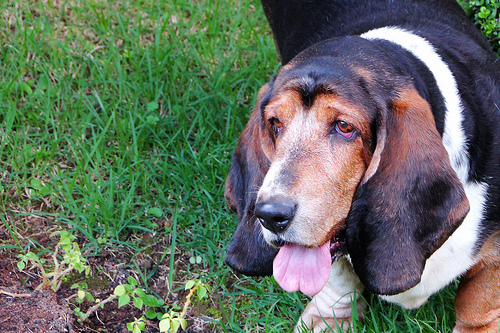
\includegraphics[width=0.40\linewidth]{imagens/basset_hound_17.jpg} &
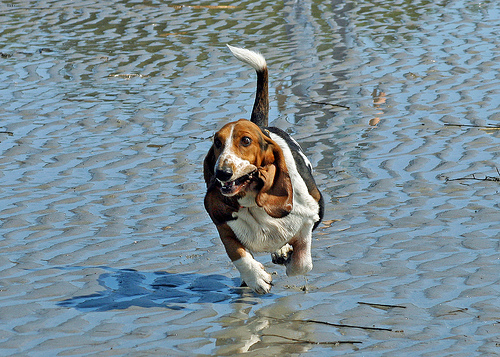
\includegraphics[width=0.40\linewidth]{imagens/basset_hound_106.jpg} \\[2pt]
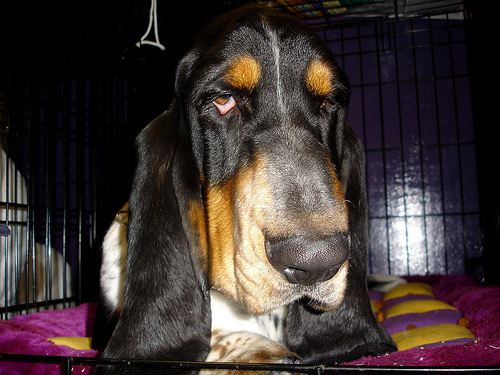
\includegraphics[width=0.40\linewidth]{imagens/basset_hound_127.jpg} &
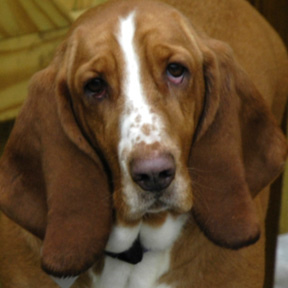
\includegraphics[width=0.40\linewidth]{imagens/basset_hound_151.jpg}
\end{tabular}
\caption{Exemplos da raça \textit{Basset Hound}.}
\end{figure}
Podemos observar que muitas vezes os padrões de cores dos cachorros da raça podem se confundir com o entorno da imagem. Além disso, temos fotos em ambientes a céu aberto e em ambientes fechados.
\begin{figure}[H]
\centering
\begin{tabular}{@{}cc@{}}
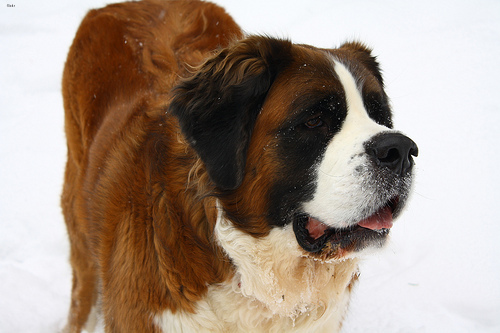
\includegraphics[width=0.40\linewidth]{imagens/saint_bernard_97.jpg} &
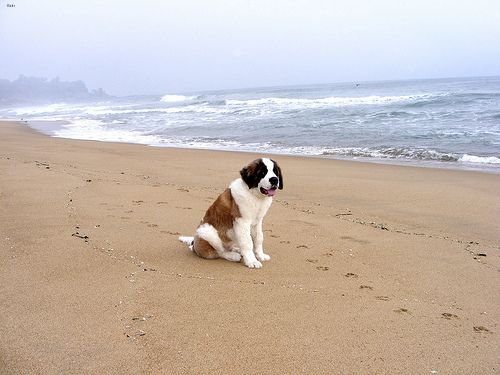
\includegraphics[width=0.40\linewidth]{imagens/saint_bernard_129.jpg} \\[2pt]
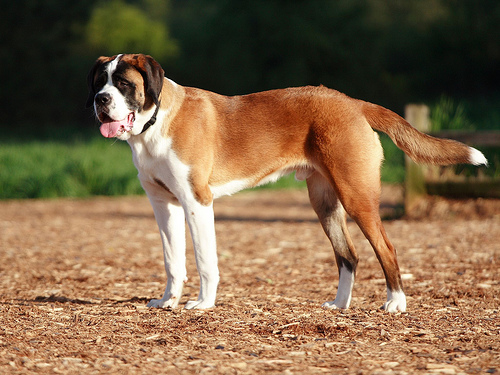
\includegraphics[width=0.40\linewidth]{imagens/saint_bernard_175.jpg} &
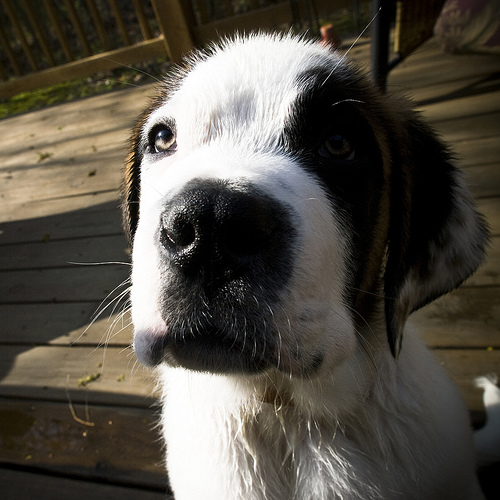
\includegraphics[width=0.40\linewidth]{imagens/saint_bernard_178.jpg}
\end{tabular}
\caption{Exemplos da raça \textit{Saint Bernard}.}
\end{figure}

\begin{figure}[H]
\centering
\begin{tabular}{@{}cc@{}}
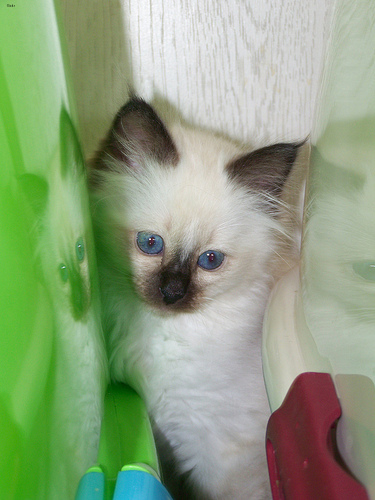
\includegraphics[width=0.30\linewidth]{imagens/Birman_1.jpg} &
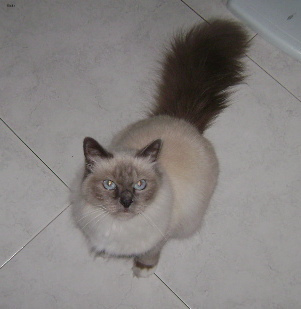
\includegraphics[width=0.30\linewidth]{imagens/Birman_55.jpg} \\[2pt]
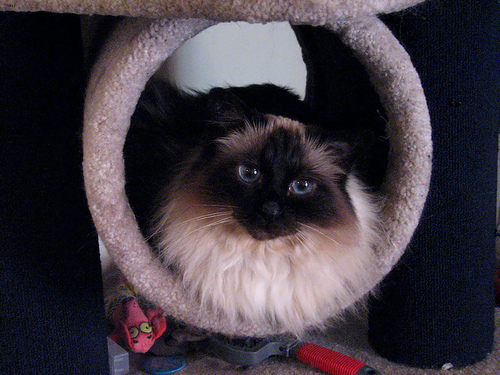
\includegraphics[width=0.30\linewidth]{imagens/Birman_66.jpg} &
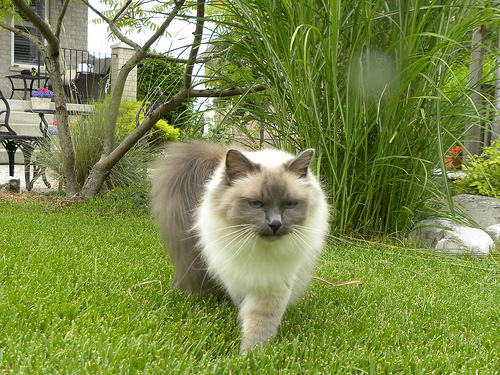
\includegraphics[width=0.30\linewidth]{imagens/Birman_145.jpg}
\end{tabular}
\caption{Exemplos da raça \textit{Birman}.}
\end{figure}

\begin{figure}[H]
\centering
\begin{tabular}{@{}cc@{}}
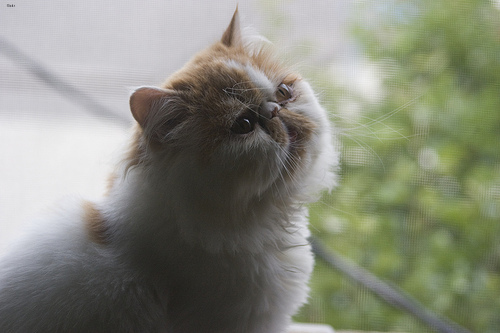
\includegraphics[width=0.40\linewidth]{imagens/Persian_89.jpg} &

\includegraphics[width=0.40\linewidth]{imagens/Persian_126.jpg} \\[2pt]
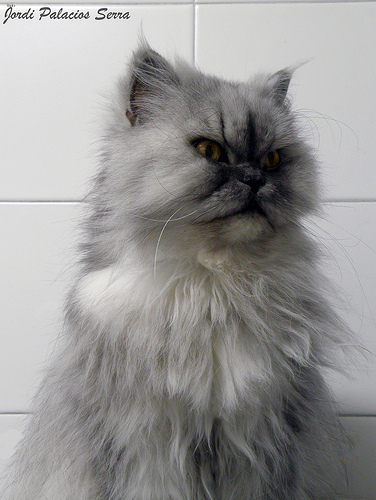
\includegraphics[width=0.40\linewidth]{imagens/Persian_169.jpg} &
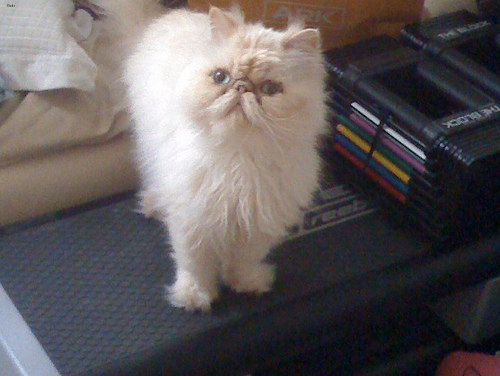
\includegraphics[width=0.40\linewidth]{imagens/Persian_181.jpg}
\end{tabular}
\caption{Exemplos da raça \textit{Persian}.}
\end{figure}

O mesmo ocorre com as demais raças de cães e gatos. Podemos também observar algumas diferenças interessantes no enquadramento. Algumas fotos não mostram o corpo completo do animal, as vezes mostrando apenas sua cabeça. Outras fotos apresentam animais jovens enquanto outras mostram animais adultos. Toda essa variabilidade contribui para avaliar a generalização da aplicação dos modelos na tarefa proposta.

Durante a etapa de extração, as imagens foram convertidas para escala de cinza e redimensionadas para dimensões fixas, garantindo consistência nas matrizes de pixels utilizadas como entrada dos extratores. Para cada imagem, foram calculados vetores de características por meio dos descritores \textit{Histogram of Oriented Gradients} (HOG) e \textit{Local Binary Pattern} (LBP), variando parâmetros como o tamanho das células, número de blocos e raio do vizinho no LBP. A combinação dessas variações resultou em múltiplas representações de cada imagem.

Em seguida, aplicou-se a técnica de redução de dimensionalidade \textit{Principal Component Analysis} (PCA) a subconjuntos dessas representações, gerando versões compactas dos vetores de características. O resultado final consistiu em 12 bases distintas — seis obtidas diretamente dos descritores HOG e LBP com diferentes parametrizações e seis derivadas de suas versões reduzidas via PCA. Cada base contém o mesmo número de amostras (800), mas dimensões e distribuições de atributos distintas, o que permite avaliar o impacto das representações sobre o desempenho dos classificadores. A seguir detalhamos o pré-processamento aplicado às imagens.

\section{Pré-processamento}

O pré-processamento consistiu na transformação das imagens originais em representações numéricas adequadas ao aprendizado supervisionado. Todas as imagens foram convertidas para escala de cinza e redimensionadas para duas resoluções fixas — \textbf{128×128} e \textbf{256×256 pixels} —, assegurando consistência dimensional entre amostras e permitindo comparar o impacto da resolução sobre o desempenho dos classificadores.  

\subsection{Extração de características}

Foram empregados dois descritores: \textit{Histogram of Oriented Gradients} (HOG) e \textit{Local Binary Pattern} (LBP). Ambos foram aplicados de forma sistemática, com variações paramétricas destinadas a capturar diferentes propriedades estruturais e texturais das imagens. As configurações foram definidas conforme as definições a seguir:

\subsubsection{Descritor HOG}

O descritor HOG foi configurado para representar as variações locais de intensidade por meio da distribuição dos gradientes direcionais. As variações experimentadas consideraram diferentes granularidades espaciais e tamanhos de bloco, permitindo avaliar o impacto da discretização na representação estrutural.

\begin{table}[H]
\centering
\caption{Parâmetros utilizados para o extrator HOG}
\label{tab:hog_parametros}
\begin{tabular}{lcc}
\toprule
\textbf{Parâmetro} & \textbf{Descrição} & \textbf{Valores utilizados} \\
\midrule
\texttt{orientations} & Número de direções de gradiente & 9 \\
\texttt{pixels\_per\_cell} & Tamanho da célula em pixels & (4,4), (8,8), (16,16) \\
\texttt{cells\_per\_block} & Número de células por bloco & (1,1), (2,2), (3,3) \\
\texttt{block\_norm} & Método de normalização dos blocos & L2-Hys \\
\texttt{transform\_sqrt} & Normalização prévia por raiz quadrada & True \\
\texttt{feature\_vector} & Saída vetorial concatenada & True \\
\bottomrule
\end{tabular}
\end{table}

As combinações entre \texttt{pixels\_per\_cell} e \texttt{cells\_per\_block} geraram nove configurações distintas, aplicadas nas duas resoluções (128×128 e 256×256). Cada vetor HOG resultante foi normalizado na faixa [0,1] antes de ser utilizado nos classificadores supervisionados.

\subsubsection{Descritor LBP}

O descritor LBP foi utilizado para representar padrões de textura locais, baseando-se na codificação binária das vizinhanças de cada pixel. O método adotado foi o \textit{uniform}, que reduz a dimensionalidade ao agrupar padrões de transição semelhantes.

\begin{table}[H]
\centering
\caption{Parâmetros utilizados para o extrator LBP}
\label{tab:lbp_parametros}
\begin{tabular}{lcc}
\toprule
\textbf{Parâmetro} & \textbf{Descrição} & \textbf{Valores utilizados} \\
\midrule
\texttt{method} & Tipo de codificação binária & uniform \\
\texttt{radius} & Raio de vizinhança & 1, 2, 3, 4 \\
\texttt{n\_points} & Número de pontos vizinhos & 8, 16, 24, 32 \\
\texttt{normalize} & Normalização do histograma & [0,1] \\
\bottomrule
\end{tabular}
\end{table}

Cada histograma LBP foi normalizado para a faixa [0,1] e convertido em vetor unidimensional. Assim como no HOG, as combinações de parâmetros foram avaliadas nas duas resoluções, totalizando oito variações por extrator.

\subsection{Redução de dimensionalidade}

Após a extração das características, as representações foram submetidas opcionalmente à técnica \textit{Principal Component Analysis} (PCA). Antes do PCA, todas as features foram normalizadas utilizando o \textit{StandardScaler}, garantindo média zero e variância unitária. O PCA foi configurado para reter \textbf{95\% da variância explicada}, reduzindo a dimensionalidade das bases sem perda significativa de informação.

\begin{table}[H]
\centering
\caption{Configuração do PCA aplicado às bases derivadas}
\label{tab:pca_parametros}
\begin{tabular}{lcc}
\toprule
\textbf{Parâmetro} & \textbf{Descrição} & \textbf{Valor} \\
\midrule
\texttt{scaler} & Normalização prévia & StandardScaler (média=0, var=1) \\
\texttt{n\_components} & Variância explicada preservada & 95\% \\
\texttt{svd\_solver} & Método de decomposição & auto \\
\bottomrule
\end{tabular}
\end{table}

\subsection{Composição e avaliação das bases derivadas}

A combinação das resoluções (128×128 e 256×256), dos dois descritores (HOG e LBP), de suas variações paramétricas e da aplicação opcional do PCA resultou em \textbf{20 bases de dados} iniciais. Cada base contém 800 amostras (400 cães e 400 gatos) e um vetor de características representando cada imagem.

Essas bases foram avaliadas segundo o desempenho do classificador \textit{k-Nearest Neighbors} (k-NN), variando o número de vizinhos \( K \in [1,10] \), sob duas estratégias de validação: \textbf{Holdout (90/10)} e \textbf{k-Fold (k=10)}. A métrica utilizada foi o \textit{F1-score}, cuja média serviu de critério para ranqueamento das bases.

\begin{landscape}
\begin{table}[H]
\centering
\caption{Resumo das 20 bases de dados avaliadas — combinações de descritores, resoluções e parâmetros utilizados}
\label{tab:bases_iniciais}
\vspace{0.5em}

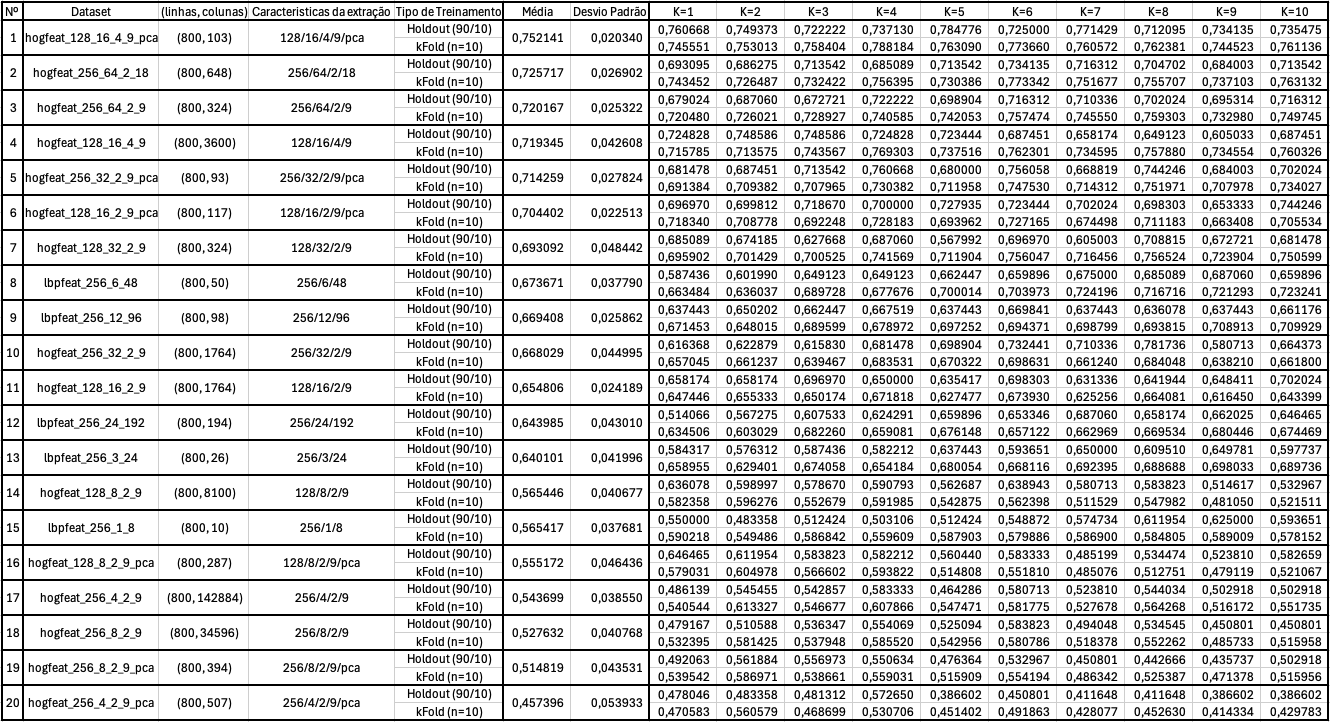
\includegraphics[width=\linewidth,height=\textheight,keepaspectratio]{tabelas/Tabela-4-selecao-datasets.png}

\vspace{0.5em}
\footnotesize
\textbf{Legenda:}  
Características da extração: LBP $\rightarrow$ Resolução/Raio/Pontos;  
HOG $\rightarrow$ Resolução/Pixels por Célula/Células por Bloco/Orientações/PCA.
\end{table}
\end{landscape}



Após a avaliação, as \textbf{12 melhores bases} foram selecionadas conforme a média de \textit{F1-score} obtida nos experimentos. Essas bases foram mantidas para as etapas seguintes de aprendizado supervisionado e de comitês de classificadores.

\begin{table}[H]
\centering
\caption{Melhores 12 bases de dados selecionadas}
\label{tab:bases_selecionadas}
\begin{tabular}{cccc}
\toprule
\textbf{Nº} & \textbf{Dataset} & \textbf{(Linhas, Colunas)} & \textbf{Características da extração} \\
\midrule
1  & hogfeat\_128\_16\_4\_9\_pca & (800, 103)   & 128/16/4/9/pca \\
2  & hogfeat\_256\_64\_2\_18     & (800, 648)   & 256/64/2/18 \\
3  & hogfeat\_256\_64\_2\_9      & (800, 324)   & 256/64/2/9 \\
4  & hogfeat\_128\_16\_4\_9      & (800, 3600)  & 128/16/4/9 \\
5  & hogfeat\_256\_32\_2\_9\_pca & (800, 93)    & 256/32/2/9/pca \\
6  & hogfeat\_128\_16\_2\_9\_pca & (800, 117)   & 128/16/2/9/pca \\
7  & hogfeat\_128\_32\_2\_9      & (800, 324)   & 128/32/2/9 \\
8  & lbpfeat\_256\_6\_48         & (800, 50)    & 256/6/48 \\
9  & lbpfeat\_256\_12\_96        & (800, 98)    & 256/12/96 \\
10 & hogfeat\_256\_32\_2\_9      & (800, 1764)  & 256/32/2/9 \\
11 & hogfeat\_128\_16\_2\_9      & (800, 1764)  & 128/16/2/9 \\
12 & lbpfeat\_256\_24\_192       & (800, 194)   & 256/24/192 \\
\bottomrule
\end{tabular}

\vspace{0.5em}
\footnotesize
\textbf{Legenda:}  
Características da extração: LBP $\rightarrow$ Resolução/Raio/Pontos;  
HOG $\rightarrow$ Resolução/Pixels por Célula/Células por Bloco/Orientações/PCA.
\end{table}


Essas tabelas sintetizam o processo de geração, avaliação e seleção das bases de dados, permitindo rastreabilidade entre as combinações de parâmetros, os resultados obtidos e as bases empregadas nas etapas subsequentes de aprendizado supervisionado e comitês de classificadores. As 12 bases selecionadas representam diferentes níveis de granularidade e abstração: algumas priorizam maior detalhamento espacial dos gradientes (como as variações HOG com células menores e blocos maiores), enquanto outras enfatizam descrições mais compactas com redução de dimensionalidade via PCA. No caso dos descritores LBP, as variações contemplam diferentes raios e números de vizinhos, capturando padrões de textura de baixa e alta frequência. Assim, o conjunto final cobre desde representações mais densas e estruturais até descrições mais reduzidas e texturais, oferecendo diversidade suficiente para análise comparativa entre classificadores e técnicas de comitês.


\section{Metodologia dos Experimentos}

Esta seção descreve como os experimentos foram conduzidos após o pré-processamento e a extração de características apresentadas anteriormente. O foco recai sobre o protocolo de particionamento dos dados, o treinamento e avaliação dos modelos supervisionados e a construção dos comitês de classificadores, garantindo comparabilidade e reprodutibilidade dos resultados.

\begin{figure}[H]
  \centering
  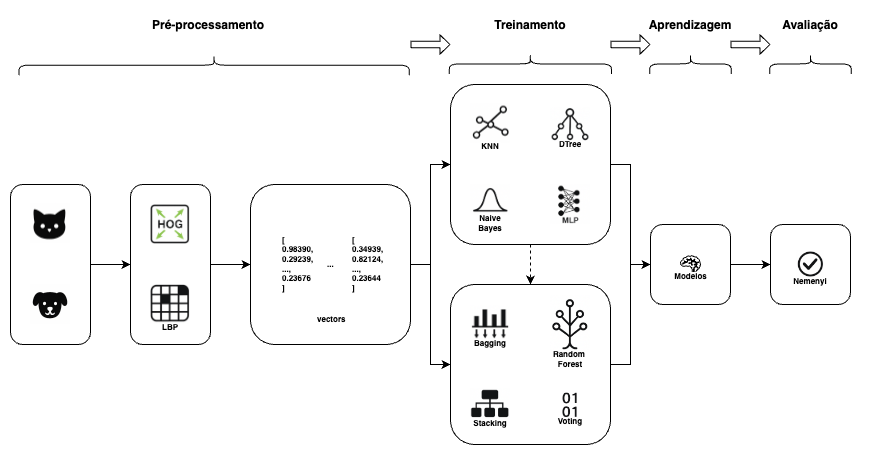
\includegraphics[width=0.95\linewidth]{imagens/metodologia-imd3002.png}
  \caption{Visão geral da metodologia experimental, desde a extração de características até a análise estatística dos resultados.}
  \label{fig:metodologia}
\end{figure}


\subsection{Protocolo de Particionamento e Avaliação}

Foram adotados dois tipos de treinamento:
\begin{enumerate}
    \item \textbf{Holdout (80/20)} — 80\% das amostras destinadas ao treinamento e 20\% ao teste (\texttt{test\_size = 0.2}). Essa divisão foi aplicada em todos os experimentos iniciais, com embaralhamento e semente fixa (\texttt{random\_state = 42}).
    \item \textbf{Validação cruzada \(k\)-fold} — utilizada com \(k = 10\), embaralhamento ativado (\texttt{shuffle=True}) e a mesma semente fixa. Foram calculadas a média e o desvio padrão do \textit{F1-score}.
\end{enumerate}

A métrica de avaliação utilizada em todas as etapas foi o \textit{F1-score} ponderado (\textit{weighted}).  
Para cada configuração de modelo ou comitê, o valor final considerado correspondeu à \textbf{média simples entre o desempenho obtido no \textit{holdout} e na validação cruzada 10-fold}, garantindo equilíbrio entre a estabilidade estatística e a capacidade de generalização observada em uma partição independente.  
Nos experimentos realizados com \textit{holdout}, também foram obtidas matrizes de confusão para detalhar os erros de classificação e avaliar a distribuição das predições por classe.

\subsection{Classificadores Supervisionados}

Foram empregados quatro algoritmos de aprendizado supervisionado: \(k\)-Nearest Neighbors (k-NN), Árvore de Decisão (DT), Naive Bayes (NB) e Multi-Layer Perceptron (MLP).  
A metodologia adotada para cada técnica foi estruturada em duas fases complementares: (i) a \textbf{busca de configurações} (\textit{Grid Search}) e (ii) a \textbf{avaliação das melhores configurações}.  

A fase de \textit{Grid Search} foi conduzida exclusivamente sobre a \textbf{base mais promissora (top 1)}, utilizando o método \textit{holdout} 80/20. Nessa etapa, variaram-se sistematicamente os hiperparâmetros de cada técnica com o objetivo de identificar as combinações com maior \textit{F1-score} médio. As dez melhores configurações foram selecionadas para a etapa seguinte.  

Na segunda fase, essas dez configurações foram reaplicadas sobre as doze bases selecionadas e avaliadas por ambas as estratégias de validação — \textit{holdout} 80/20 e validação cruzada 10-fold — sob o mesmo protocolo (com \texttt{random\_state = 42} e \texttt{shuffle=True}).  
O desempenho final de cada configuração foi calculado como a \textbf{média simples entre os valores de \textit{F1-score} obtidos nas duas estratégias}, garantindo consistência entre precisão e estabilidade de avaliação.

\begin{enumerate}
    \item \textbf{\(k\)-Nearest Neighbors (k-NN)} — O \textit{Grid Search} variou o número de vizinhos \(k \in [1,10]\), as métricas de distância Euclidiana, Manhattan e Chebyshev, e os esquemas de ponderação \textit{uniform} e \textit{distance}. As dez melhores combinações identificadas na base top 1 foram reavaliadas sobre todas as bases utilizando \textit{holdout} e validação cruzada 10-fold.

    \item \textbf{Árvore de Decisão (DT)} — O \textit{Grid Search} foi realizado variando o critério de impureza (\textit{gini}, \textit{entropy}) e a profundidade máxima da árvore (\textit{max\_depth}) de 1 a 14, totalizando 28 combinações. As dez melhores configurações obtidas no \textit{holdout} sobre a base top 1 foram reavaliadas nas doze bases com as duas estratégias de validação.

    \item \textbf{Naive Bayes (NB)} — Foram comparadas três variantes do modelo: \textit{GaussianNB}, \textit{MultinomialNB} e \textit{ComplementNB}.  
    Durante os experimentos, foi identificado um problema específico nas bases em que o método de redução de dimensionalidade PCA foi aplicado. O PCA pode gerar valores negativos, e tanto o \textit{MultinomialNB} quanto o \textit{ComplementNB} não aceitam entradas negativas, o que resultava em falhas de processamento ou desempenho incorreto.  
    Para contornar essa limitação, os dados dessas bases foram escalonados para o intervalo \([0,1]\). Essa normalização preservou as relações entre os atributos e garantiu compatibilidade com todos os classificadores NB, permitindo a execução consistente sobre todas as bases avaliadas.  
    Após esse ajuste, as variantes foram reavaliadas, e as duas de melhor desempenho foram selecionadas para aplicação nas demais bases, considerando simultaneamente \textit{holdout} e validação cruzada 10-fold.

    \item \textbf{Multi-Layer Perceptron (MLP)} — O processo de busca de configurações para o MLP exigiu modificações metodológicas.  
    Devido à grande variação na quantidade de atributos entre as diferentes bases, observou-se que algumas configurações apresentavam ótimo desempenho em bases com poucos atributos, mas desempenho inferior em bases com muitos atributos, e vice-versa.  
    Além disso, verificou-se que o parâmetro \textit{max\_iter}, quando incluído como variável no \textit{Grid Search}, gerava distorções: configurações idênticas, diferenciadas apenas pelo número de iterações (500, 1000, 1500), ocupavam várias das primeiras posições do ranking por apresentarem convergência rápida, concentrando os melhores resultados em um mesmo tipo de modelo.  

    Assim, a estratégia de busca foi adaptada para cobrir de forma mais equilibrada os dois cenários observados. Foram selecionadas as \textbf{cinco melhores configurações com menor número de iterações} (modelos mais simples e rápidos, adequados a bases com poucos atributos) e as \textbf{cinco melhores com maior número de iterações} (modelos mais complexos, adequados a bases com muitos atributos).  
    Essa adaptação aumentou a diversidade entre os modelos avaliados e proporcionou uma cobertura mais equilibrada do espaço de configurações, evitando a concentração de resultados redundantes e refletindo melhor a influência da dimensionalidade das bases no desempenho da rede.  
    As dez configurações finais obtidas foram posteriormente reavaliadas em todas as bases, aplicando \textit{holdout} e validação cruzada 10-fold, consolidando-se o desempenho médio de cada configuração.
\end{enumerate}

\subsection{Comitês de Classificadores}

Os comitês foram construídos a partir das melhores configurações dos classificadores base, aplicando-se o mesmo protocolo de validação dupla (\textit{holdout} 80/20 e 10-fold) e consolidando o resultado final pela média simples entre ambos.  
Foram implementadas quatro estruturas — Bagging, Random Forest, Voting e Stacking —, cada uma avaliada de forma independente e comparada em termos de desempenho médio e estabilidade.

\begin{itemize}
    \item \textbf{Bagging} — Implementado com os classificadores base \(k\)-NN, Árvore de Decisão, Naive Bayes e MLP. O número de modelos em cada comitê variou entre 10, 15 e 20, mantendo os demais parâmetros em seus valores padrão. Cada configuração foi avaliada tanto em \textit{holdout} quanto em validação cruzada 10-fold, sendo o desempenho final obtido pela média simples entre ambas as medidas.

    \item \textbf{Random Forest} — Utilizou como base árvores de decisão, com critérios de impureza \textit{gini} e \textit{entropy}, e número de árvores igual a 10, 20, 30 e 100. O mesmo protocolo de validação dupla foi adotado, possibilitando a análise conjunta de desempenho médio e custo computacional.

    \item \textbf{Voting} — Comitê heterogêneo formado pelos classificadores \(k\)-NN, Árvore de Decisão e MLP. Foram avaliados tamanhos de comitê de 5, 10, 15 e 20 modelos, combinando variações específicas de cada técnica de acordo com as configurações que apresentaram melhor desempenho nos experimentos individuais.  
    O mecanismo de decisão adotado foi a votação ponderada por probabilidade (\textit{soft voting}), o que permite considerar o grau de confiança das predições de cada classificador. Essa abordagem favoreceu o equilíbrio entre modelos de diferentes naturezas e complexidades, mantendo consistência nos resultados mesmo em bases com diferentes dimensionalidades.

    \item \textbf{Stacking} — Estrutura heterogênea também composta pelos classificadores \(k\)-NN, Árvore de Decisão e MLP, com tamanhos de comitê de 5, 10, 15 e 20 modelos. Assim como no Voting, foram utilizadas as melhores variações de cada classificador individual identificadas anteriormente.  
    O meta-classificador empregado foi um modelo linear supervisionado, responsável por combinar as saídas probabilísticas dos classificadores de base e gerar a predição final. Esse arranjo permitiu explorar complementaridades entre os métodos e reduzir a variância dos resultados.  
\end{itemize}

Os resultados de cada comitê foram comparados entre si e em relação aos classificadores individuais, permitindo avaliar ganhos em desempenho e robustez decorrentes das estratégias de agregação e da diversidade dos modelos.


\subsection{Análise Estatística}

Os resultados dos classificadores individuais e dos comitês foram submetidos a testes estatísticos não paramétricos. Inicialmente, aplicou-se o teste de Friedman para verificar a existência de diferenças significativas entre os métodos (\(p < 0{,}05\)). Quando a hipótese nula foi rejeitada, aplicou-se o teste post-hoc de Nemenyi para comparações múltiplas entre pares, identificando quais modelos apresentaram diferenças estatísticas significativas.

\subsection{Reprodutibilidade}

Todas as rotinas empregaram \texttt{random\_state = 42} para garantir consistência nas divisões de dados e replicabilidade dos resultados. O protocolo de avaliação, as métricas e o procedimento de reavaliação das melhores configurações foram mantidos idênticos em todas as bases e classificadores.



\section{Resultados Experimentais}

\subsection{Visão Geral dos Resultados}

\subsubsection{Panorama dos Classificadores Individuais}

Os experimentos com os classificadores individuais permitiram analisar o impacto dos parâmetros internos e do tipo de descritor sobre o desempenho médio de classificação. De forma geral, os modelos supervisionados apresentaram comportamentos consistentes e coerentes com suas propriedades teóricas. O \textit{k-Nearest Neighbors} (k-NN) mostrou desempenho estável, com médias em torno de 0,60 no F1-score, destacando-se pela simplicidade e previsibilidade, embora limitado em bases de alta dimensionalidade. A \textit{Árvore de Decisão} apresentou melhoria expressiva em relação ao k-NN, atingindo cerca de 0,67 em média, evidenciando sua capacidade de capturar relações não lineares entre atributos.

O \textit{Naive Bayes} apresentou desempenho superior aos dois anteriores, com média de F1 próxima de 0,74, especialmente na variante \textit{GaussianNB}, que se mostrou mais adequada às distribuições contínuas derivadas dos descritores HOG e LBP. Por fim, o \textit{Multi-Layer Perceptron} (MLP) obteve o maior desempenho entre os classificadores individuais, alcançando média de 0,76 no F1-score, confirmando sua capacidade de representar relações complexas e generalizar de forma consistente. A análise conjunta demonstrou que o aumento da complexidade do modelo esteve diretamente associado ao ganho de desempenho, embora acompanhado por maior custo computacional.

\subsubsection{Panorama dos Comitês de Classificadores}

Os comitês de classificadores apresentaram desempenho médio superior aos modelos individuais, reforçando a eficiência das estratégias de combinação. O \textit{Bagging} destacou-se como método de estabilização, aumentando a robustez dos modelos de maior variância, especialmente a \textit{Árvore de Decisão}, e atingindo média de F1 próxima de 0,77. O \textit{Random Forest}, ao incorporar aleatorização de atributos, manteve resultados próximos ($F1 \approx 0,76$), com excelente equilíbrio entre acurácia, estabilidade e custo computacional.

Entre os comitês heterogêneos, o \textit{Voting} apresentou média de F1 de 0,75, com variação moderada e tempo de execução reduzido, demonstrando bom desempenho em relação à sua simplicidade estrutural. Já o \textit{Stacking} apresentou desempenho semelhante ao \textit{Bagging} ($F1 \approx 0,77$), destacando-se pela consistência inter-bases e pela baixa variância dos resultados. No conjunto, observou-se que o ganho médio de desempenho entre os comitês em relação aos classificadores individuais foi discreto, mas acompanhado por redução significativa na variabilidade dos resultados, indicando melhor generalização e estabilidade.


\subsubsection{Síntese Estatística Inicial (Testes de Friedman e Nemenyi)}

Os testes estatísticos iniciais confirmaram as tendências observadas nos resultados médios. Para os classificadores individuais, o teste de Friedman indicou diferenças estatisticamente significativas ($p < 10^{-10}$), e o teste post-hoc de Nemenyi revelou a superioridade do MLP frente aos demais modelos, com diferenças significativas em relação ao k-NN, à Árvore de Decisão e ao Naive Bayes. Esses resultados sustentam a escolha do MLP como referência para as etapas subsequentes de comparação com os comitês.

Nos comitês de classificadores, o teste de Friedman ($p = 0{,}489$) não identificou diferenças estatísticas significativas entre as melhores configurações de \textit{Bagging}, \textit{Random Forest}, \textit{Voting} e \textit{Stacking}, demonstrando que todas as abordagens apresentaram desempenhos equivalentes dentro do intervalo de confiança adotado. A homogeneidade estatística sugere que, embora as estruturas variem em complexidade, convergem para níveis semelhantes de acurácia e estabilidade quando aplicadas ao mesmo conjunto de dados.

Assim, esta visão geral sintetiza o comportamento global dos métodos avaliados e estabelece as bases para as análises detalhadas subsequentes, nas quais cada técnica é examinada individualmente quanto aos efeitos de seus parâmetros, descritores e protocolos de validação.

\subsection{Análise Detalhada dos Classificadores Individuais}

\subsubsection{k-Nearest Neighbors (k-NN)}

Os experimentos com o algoritmo \textit{k}-Nearest Neighbors buscaram avaliar o impacto do número de vizinhos, da métrica de distância e da estratégia de ponderação sobre o desempenho médio de classificação. Foram testadas dez configurações, combinando os valores de $k = \{3, 5, 7, 11, 15\}$ e as funções de ponderação \texttt{uniform} e \texttt{distance}. 

Durante a etapa de \textit{grid search}, aplicada sobre a melhor base de dados selecionada, todas as configurações de maior desempenho utilizaram a métrica de distância \texttt{chebyshev}. Esse resultado reflete características específicas dessa base, que apresenta variabilidade concentrada em poucos atributos de grande amplitude. Como a distância de Chebyshev é definida pelo maior valor absoluto de diferença entre as dimensões correspondentes dos vetores, ela tende a enfatizar os atributos dominantes em magnitude, resultando em uma separação mais clara entre as classes nesse conjunto em particular.

A Tabela~\ref{tab:knn-config} apresenta as configurações avaliadas no experimento.

\begin{table}[H]
\centering
\caption{Configurações avaliadas para o classificador k-NN.}
\label{tab:knn-config}
\begin{tabular}{lc}
\toprule
\textbf{Configuração} & \textbf{Parâmetros} \\
\midrule
1 & \{\texttt{metric}: chebyshev, \texttt{n\_neighbors}: 3, \texttt{weights}: distance\} \\
2 & \{\texttt{metric}: chebyshev, \texttt{n\_neighbors}: 3, \texttt{weights}: uniform\} \\
3 & \{\texttt{metric}: chebyshev, \texttt{n\_neighbors}: 5, \texttt{weights}: distance\} \\
4 & \{\texttt{metric}: chebyshev, \texttt{n\_neighbors}: 5, \texttt{weights}: uniform\} \\
5 & \{\texttt{metric}: chebyshev, \texttt{n\_neighbors}: 11, \texttt{weights}: distance\} \\
6 & \{\texttt{metric}: chebyshev, \texttt{n\_neighbors}: 11, \texttt{weights}: uniform\} \\
7 & \{\texttt{metric}: chebyshev, \texttt{n\_neighbors}: 15, \texttt{weights}: distance\} \\
8 & \{\texttt{metric}: chebyshev, \texttt{n\_neighbors}: 15, \texttt{weights}: uniform\} \\
9 & \{\texttt{metric}: chebyshev, \texttt{n\_neighbors}: 7, \texttt{weights}: distance\} \\
10 & \{\texttt{metric}: chebyshev, \texttt{n\_neighbors}: 7, \texttt{weights}: uniform\} \\
\bottomrule
\end{tabular}
\end{table}

\begin{landscape}
\begin{table}[H]
\centering
\caption{Médias de \textit{F1-score} por configuração e base de dados para o classificador k-NN.}
\label{tab:knn-matrix}
\vspace{0.5em}

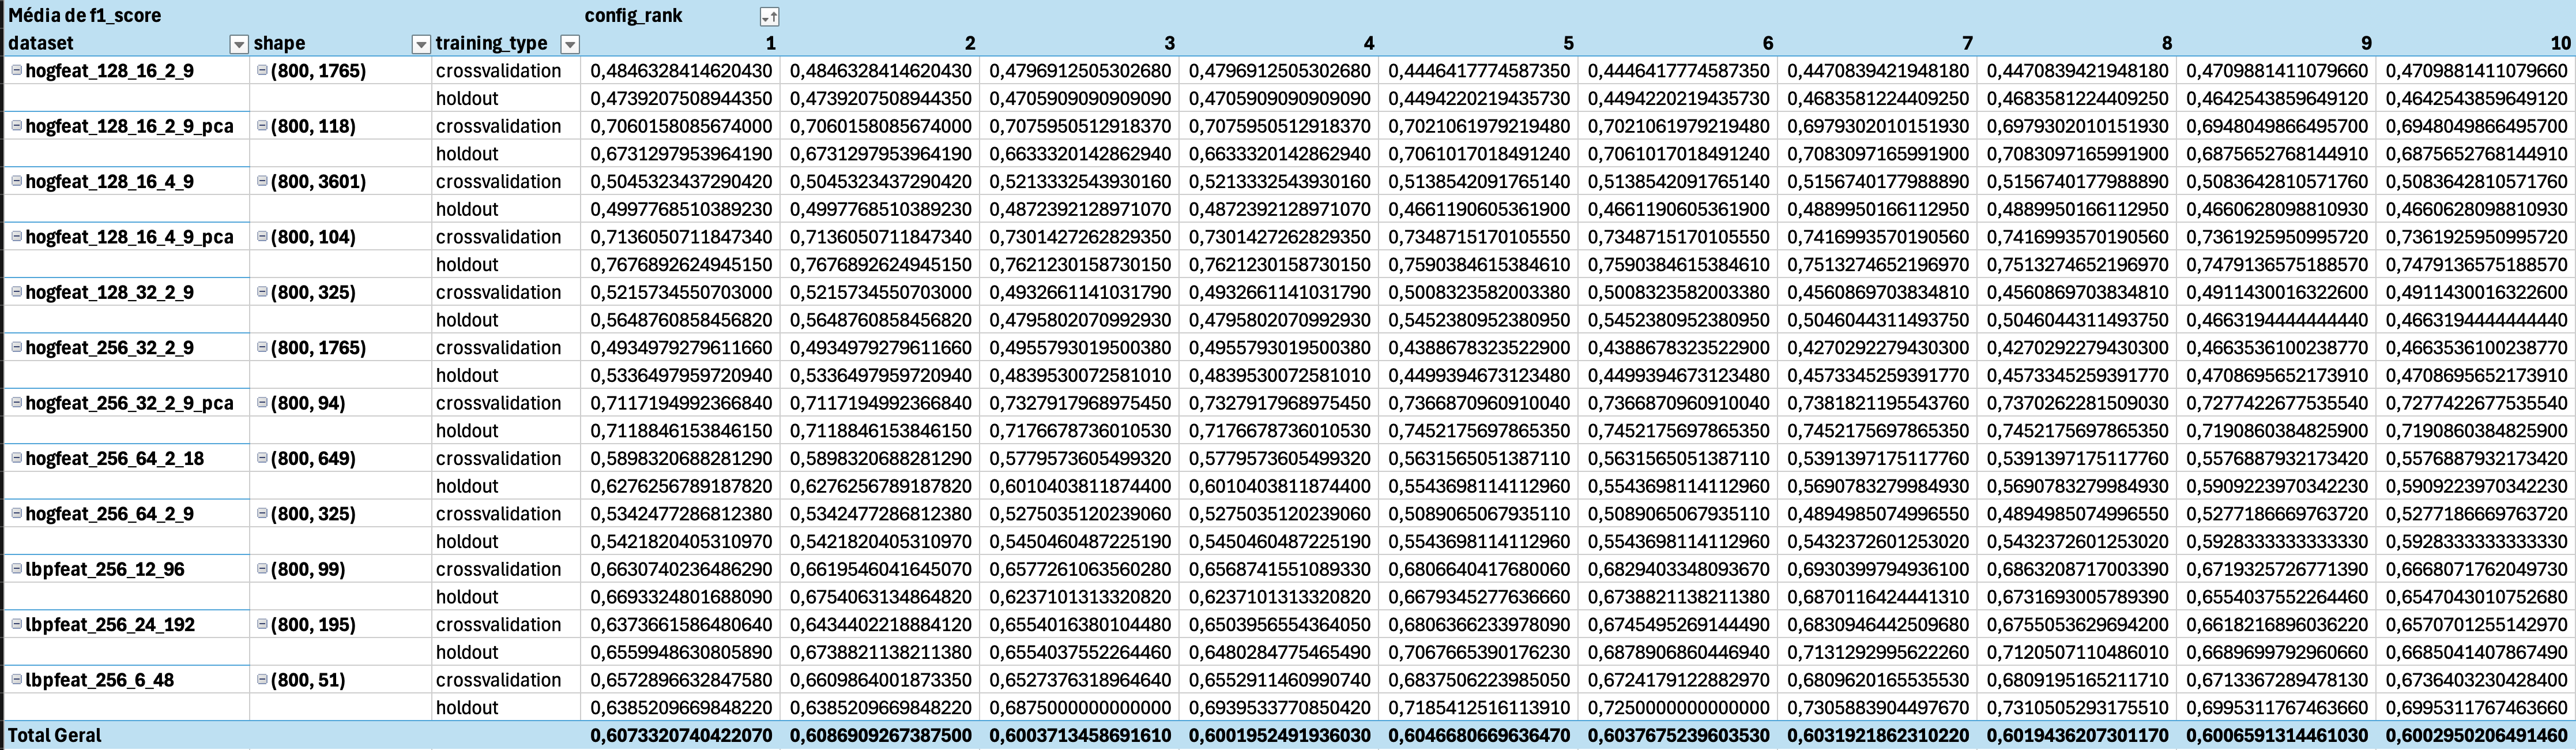
\includegraphics[width=\linewidth,height=\textheight,keepaspectratio]{tabelas/knn-matrix.png}

\vspace{0.5em}
\footnotesize
\textbf{Legenda:} cada coluna representa uma configuração distinta de $k$ e função de ponderação;  
as linhas correspondem às diferentes bases avaliadas (descritores HOG e LBP, com ou sem PCA).
\end{table}

\vspace{1em}
\normalsize

\paragraph{Comportamento dos Parâmetros.}  
A média global de desempenho foi de aproximadamente 0{,}60, com pequena vantagem do protocolo de \textit{cross-validation} em relação ao Holdout.  
As configurações com $k = 5$ e $k = 7$ (Configs 3 e 9), ambas com ponderação por distância, apresentaram os melhores resultados médios, indicando que valores intermediários de $k$ favorecem o equilíbrio entre precisão e revocação.  
Configurações com vizinhanças muito amplas ($k \geq 11$) apresentaram leve queda de desempenho, efeito típico de suavização excessiva da fronteira de decisão.
\end{landscape}

\paragraph{Influência do Tipo de Descritor e Validação}

Os resultados mostraram desempenho superior nas bases HOG em comparação às bases LBP, indicando maior separabilidade entre as classes no espaço de gradientes. As versões reduzidas por PCA mantiveram desempenho próximo às originais, demonstrando que a redução de dimensionalidade não comprometeu a capacidade discriminativa. O protocolo de \textit{cross-validation} apresentou menor desvio padrão, evidenciando estabilidade dos resultados.

\paragraph{Análise Estatística}

O teste de Friedman resultou em um valor de $p = 0{,}6153$, o que não permite rejeitar a hipótese nula de igualdade entre as configurações. Assim, as diferenças observadas entre os dez modelos avaliados não são estatisticamente significativas ao nível de 5\%.

\paragraph{Desempenho Global e Custo Computacional}

A Figura~\ref{fig:knn-rank} apresenta o desempenho consolidado das dez configurações em termos de média e desvio padrão do \textit{F1-score}, além do tempo médio de execução. As variações entre as configurações foram pequenas, com tempos próximos a 0{,}28 segundos por execução e desvios inferiores a 0{,}12 no \textit{F1-score}. Esses resultados reforçam a estabilidade do k-NN frente às mudanças moderadas de $k$ e tipo de ponderação.

\begin{figure}[H]
\centering
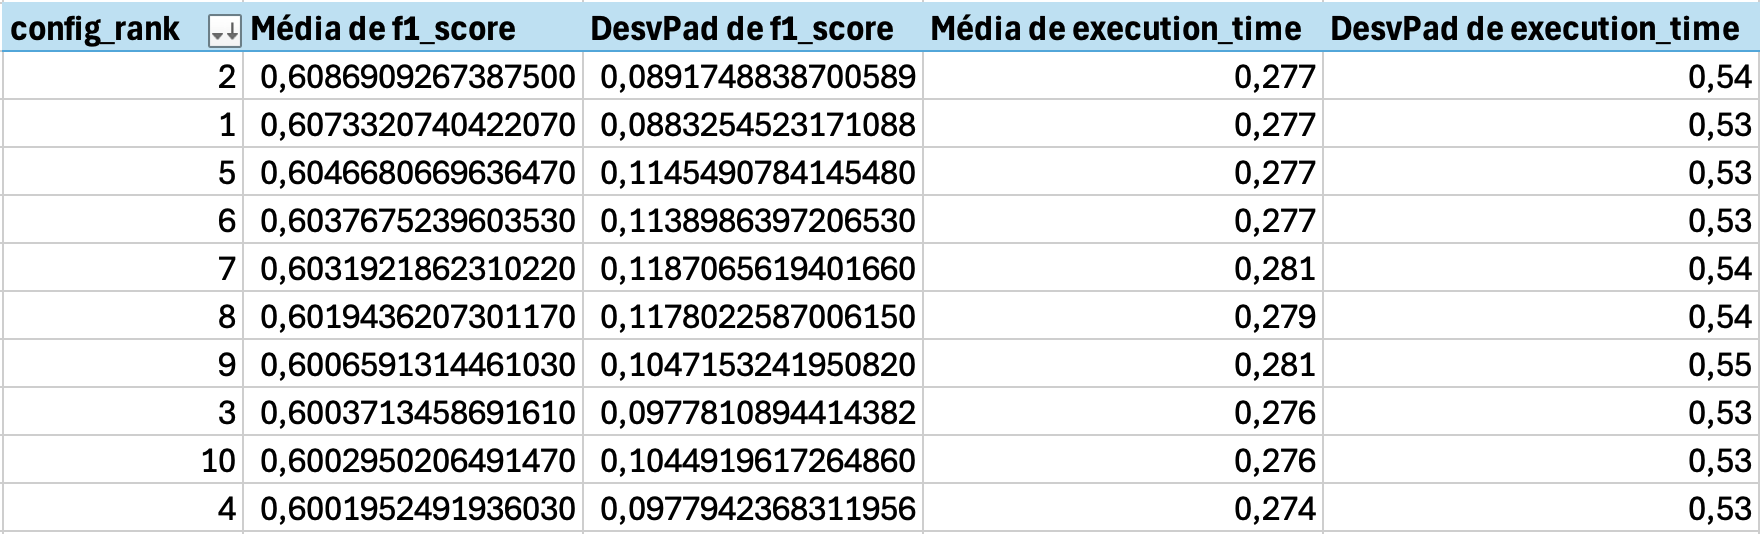
\includegraphics[width=0.9\linewidth]{tabelas/knn-rank.png}
\caption{Desempenho médio, desvio padrão e tempo de execução das dez configurações do k-NN.}
\label{fig:knn-rank}
\end{figure}

\paragraph{Interpretação dos Resultados}

Embora as diferenças não tenham sido estatisticamente significativas, observou-se tendência de melhor desempenho para configurações intermediárias de $k$ com ponderação por distância. O predomínio da métrica Chebyshev nas melhores configurações está diretamente relacionado às propriedades da base utilizada no \textit{grid search}, cujos atributos apresentam amplitudes distintas e valores concentrados em faixas específicas. Essa métrica destacou de forma mais eficaz as componentes responsáveis pela distinção entre cães e gatos, favorecendo uma separação local mais nítida. Assim, o k-NN mostrou-se adequado como modelo de referência, combinando simplicidade, baixo custo computacional e desempenho consistente.

\paragraph{Limitações e Observações}

O desempenho inferior nas bases LBP sugere sensibilidade a ruídos texturais e variação de iluminação, aspectos mais evidentes nesse tipo de descritor. Além disso, o custo de inferência aumenta com o tamanho do conjunto de treinamento, o que restringe sua aplicabilidade em bases maiores. Ainda assim, o k-NN apresentou estabilidade e resultados coerentes, servindo de parâmetro de comparação para os classificadores subsequentes.





\subsubsection{Árvore de Decisão (Decision Tree)}

Os experimentos com o algoritmo \textit{Decision Tree Classifier} tiveram como objetivo analisar a influência do critério de divisão e da profundidade máxima sobre o desempenho de classificação. Foram testadas dez configurações combinando os critérios \texttt{gini}, \texttt{entropy} e \texttt{log\_loss}, com valores de \texttt{max\_depth} variando entre 3 e 10.

A Tabela~\ref{tab:dtree-config} apresenta as configurações avaliadas no experimento.

\begin{table}[H]
\centering
\caption{Configurações avaliadas para o classificador Árvore de Decisão.}
\label{tab:dtree-config}
\begin{tabular}{lc}
\toprule
\textbf{Configuração} & \textbf{Parâmetros} \\
\midrule
1 & \{\texttt{criterion}: entropy, \texttt{max\_depth}: 3\} \\
2 & \{\texttt{criterion}: log\_loss, \texttt{max\_depth}: 3\} \\
3 & \{\texttt{criterion}: gini, \texttt{max\_depth}: 3\} \\
4 & \{\texttt{criterion}: entropy, \texttt{max\_depth}: 5\} \\
5 & \{\texttt{criterion}: log\_loss, \texttt{max\_depth}: 4\} \\
6 & \{\texttt{criterion}: entropy, \texttt{max\_depth}: 4\} \\
7 & \{\texttt{criterion}: gini, \texttt{max\_depth}: 4\} \\
8 & \{\texttt{criterion}: log\_loss, \texttt{max\_depth}: 5\} \\
9 & \{\texttt{criterion}: entropy, \texttt{max\_depth}: 10\} \\
10 & \{\texttt{criterion}: log\_loss, \texttt{max\_depth}: 9\} \\
\bottomrule
\end{tabular}
\end{table}

\begin{landscape}
\begin{table}[H]
\centering
\caption{Médias de \textit{F1-score} por configuração e base de dados para o classificador Árvore de Decisão.}
\label{tab:dtree-matrix}
\vspace{0.5em}

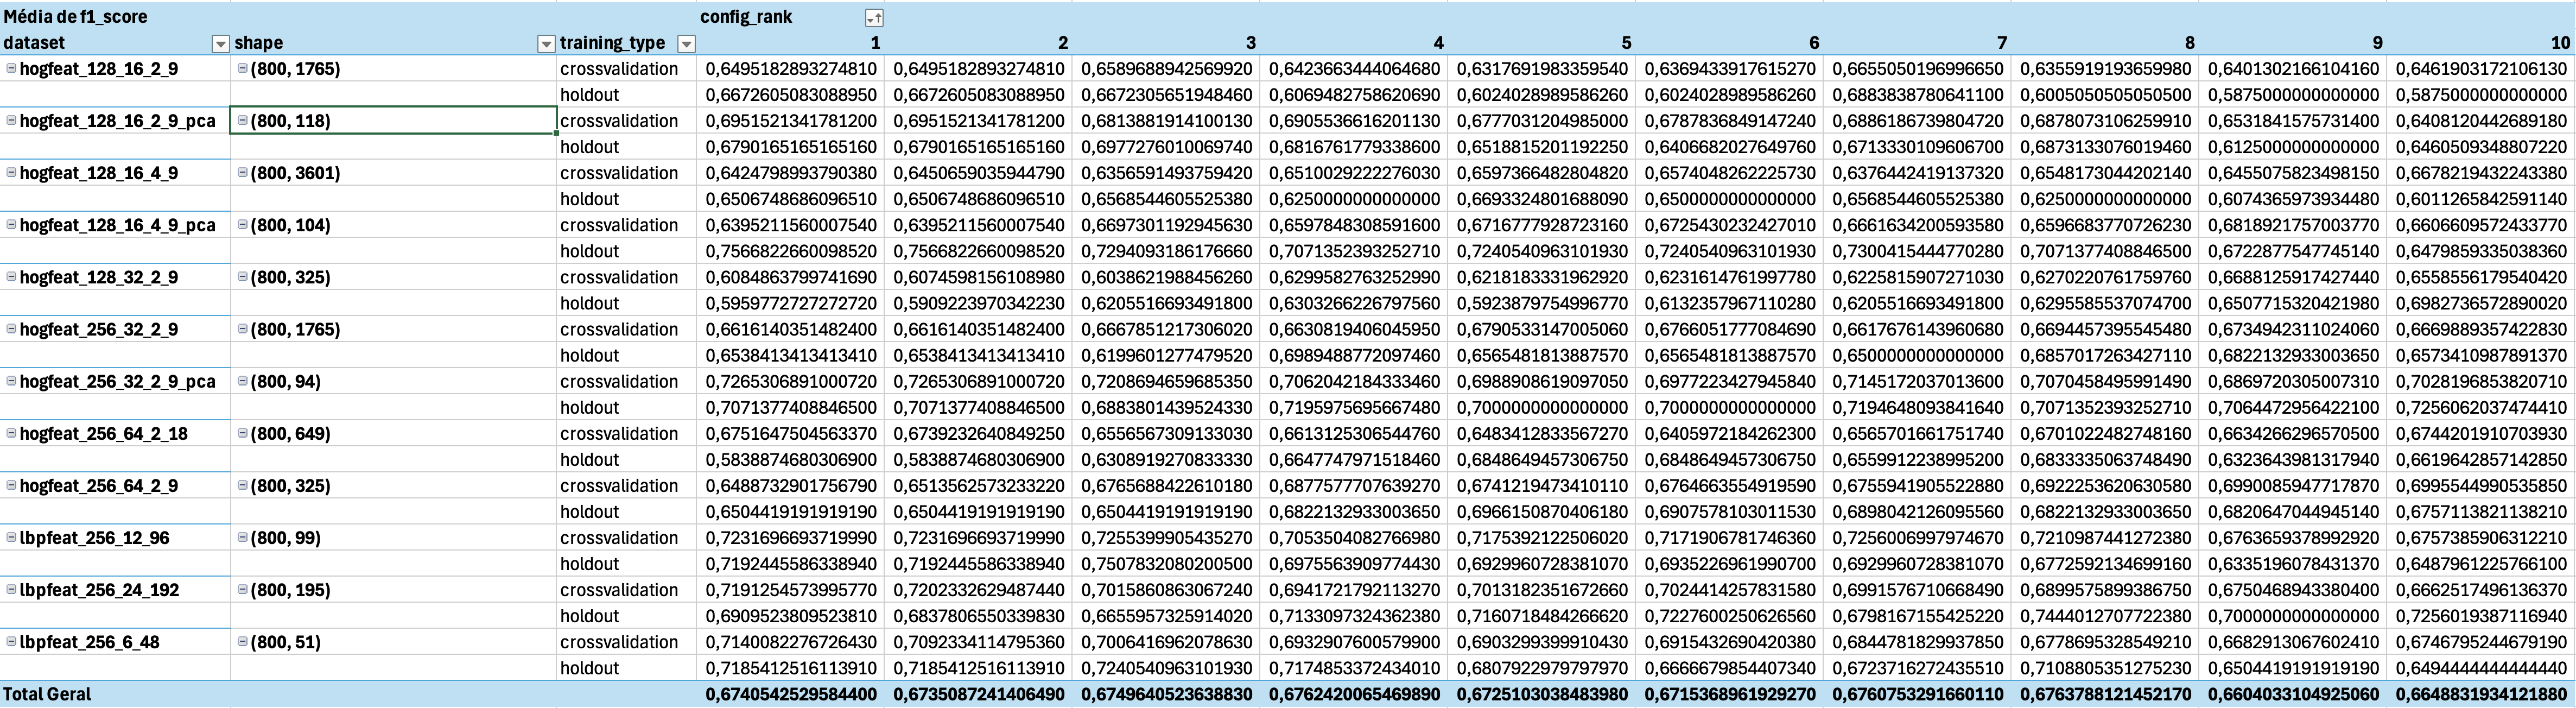
\includegraphics[width=\linewidth,height=\textheight,keepaspectratio]{tabelas/dtree-matrix.png}

\vspace{0.5em}
\footnotesize
\textbf{Legenda:} cada coluna representa uma combinação de profundidade e critério de divisão;  
as linhas correspondem às diferentes bases avaliadas (descritores HOG e LBP, com ou sem PCA).
\end{table}

\vspace{1em}
\normalsize

\paragraph{Comportamento dos Parâmetros.}  
A média global de desempenho foi de aproximadamente 0{,}67, superior à obtida pelo k-NN.  
As menores profundidades (\texttt{max\_depth} = 3–5) proporcionaram os melhores resultados, evidenciando que árvores mais rasas capturam padrões relevantes sem sobreajuste.  
Os critérios \texttt{entropy} e \texttt{log\_loss} apresentaram desempenho quase idêntico e ligeiramente superior ao \texttt{gini}, sugerindo que medidas baseadas em informação tendem a discriminar melhor as classes neste conjunto.  
Configurações com profundidade elevada ($\geq 9$) resultaram em pequenas perdas de desempenho e aumento expressivo no tempo de execução, indicando complexidade desnecessária para o volume e variabilidade dos dados.
\end{landscape}

\paragraph{Influência do Tipo de Descritor e Validação}

As bases HOG novamente apresentaram desempenho superior, com médias acima de 0{,}68, enquanto as LBP permaneceram ligeiramente abaixo de 0{,}66.  
O comportamento consistente entre as versões com e sem PCA indica que a redução de dimensionalidade preservou a separabilidade entre as classes.  
O protocolo de \textit{cross-validation} manteve resultados estáveis e maior confiabilidade, apresentando menor variância que o Holdout.

\paragraph{Análise Estatística}

O teste de Friedman resultou em um valor de $p = 0{,}7161$, não havendo evidência estatística de diferença significativa entre as dez configurações.  
Portanto, todas as variações de profundidade e critério de divisão apresentaram desempenhos comparáveis dentro do nível de significância de 5\%.

\paragraph{Desempenho Global e Custo Computacional}

A Figura~\ref{fig:dtree-rank} apresenta a consolidação das médias de \textit{F1-score}, desvios padrão e tempos de execução.  
As variações entre as configurações foram pequenas, com tempos médios entre 1 e 2{,}8 s por execução.  
Os desvios padrão do \textit{F1-score} variaram de 0{,}03 a 0{,}04, evidenciando estabilidade e reprodutibilidade do modelo.  
Mesmo as configurações mais profundas mantiveram desempenho próximo às demais, mas com aumento do custo de processamento.

\begin{figure}[H]
\centering
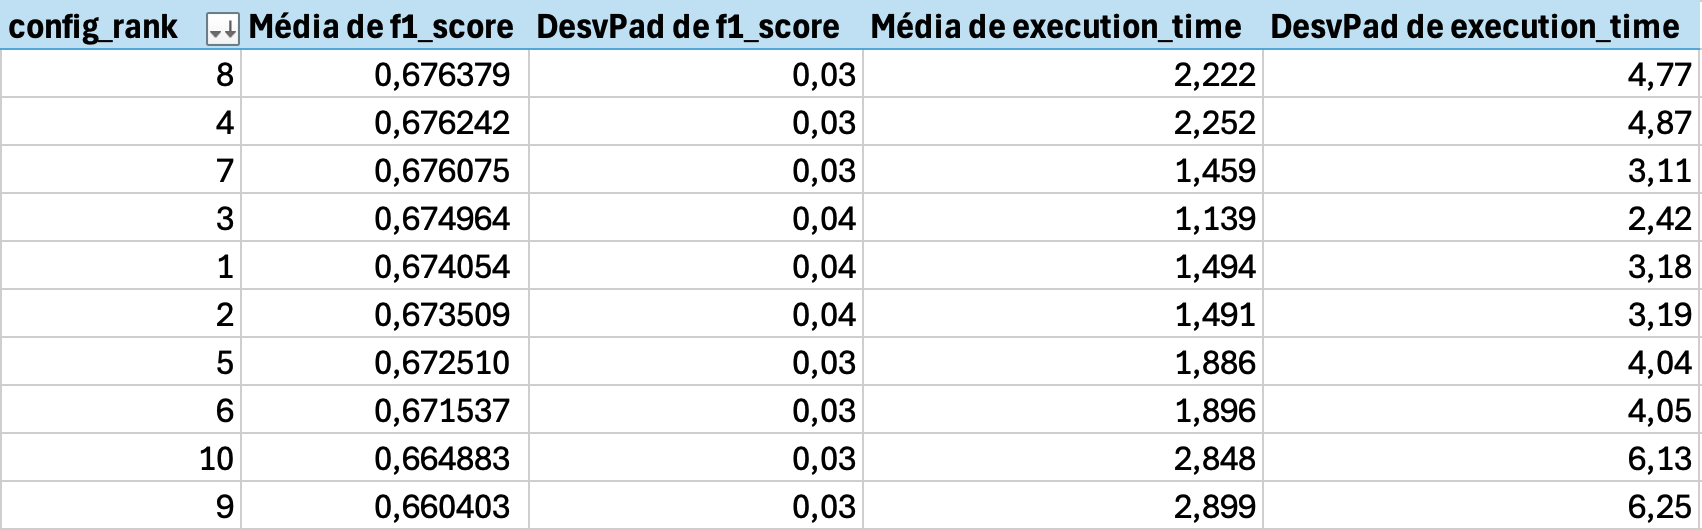
\includegraphics[width=0.9\linewidth]{tabelas/dtree-rank.png}
\caption{Desempenho médio, desvio padrão e tempo de execução das dez configurações da Árvore de Decisão.}
\label{fig:dtree-rank}
\end{figure}

\paragraph{Interpretação dos Resultados}

A análise confirma que a profundidade da árvore é o fator de maior impacto no desempenho, mas que valores intermediários oferecem o melhor equilíbrio entre precisão e generalização.  
Os critérios \texttt{entropy} e \texttt{log\_loss} destacaram-se levemente, o que indica que a medida de ganho de informação contribuiu para uma separação mais eficaz entre as classes de imagens.  
O desempenho médio superior ao k-NN sugere que a Árvore de Decisão conseguiu explorar melhor as relações não lineares entre os atributos, mantendo ainda baixo custo computacional.

\paragraph{Limitações e Observações}

As Árvores de Decisão apresentaram variação discreta entre as configurações, mas são sensíveis à profundidade e ao particionamento dos dados.  
Embora rápidas de treinar, podem gerar fronteiras instáveis quando aplicadas a dados com alta correlação entre atributos.  
Apesar disso, mostraram excelente relação entre simplicidade, interpretabilidade e desempenho, consolidando-se como um dos modelos mais equilibrados entre os classificadores testados.


\subsubsection{Naive Bayes (NB)}

Os experimentos com o classificador \textit{Naive Bayes} buscaram comparar o desempenho de suas principais variações probabilísticas na tarefa de classificação binária de imagens. Foram avaliadas três configurações distintas: \texttt{GaussianNB}, \texttt{ComplementNB} e \texttt{MultinomialNB}, representando abordagens adaptadas a diferentes distribuições de atributos.  
Esses modelos se diferenciam pelo tipo de suposição estatística sobre os dados — contínuos no caso do \texttt{GaussianNB} e discretos ou normalizados para as demais variantes.

A Tabela~\ref{tab:nb-config} apresenta as configurações avaliadas no experimento.

\begin{table}[H]
\centering
\caption{Configurações avaliadas para o classificador Naive Bayes.}
\label{tab:nb-config}
\begin{tabularx}{\textwidth}{@{}>{\centering\arraybackslash}p{1.5cm} >{\ttfamily\raggedright\arraybackslash}X@{}}
\toprule
\textbf{Config.} & \textbf{Parâmetros} \\
\midrule
1 & \{nb\_type: ComplementNB\} \\
2 & \{nb\_type: GaussianNB\} \\
3 & \{nb\_type: MultinomialNB\} \\
\bottomrule
\end{tabularx}
\end{table}

\begin{landscape}
\begin{table}[H]
\centering
\caption{Médias de \textit{F1-score} por configuração e base de dados para o classificador Naive Bayes.}
\label{tab:nb-matrix}
\vspace{0.5em}

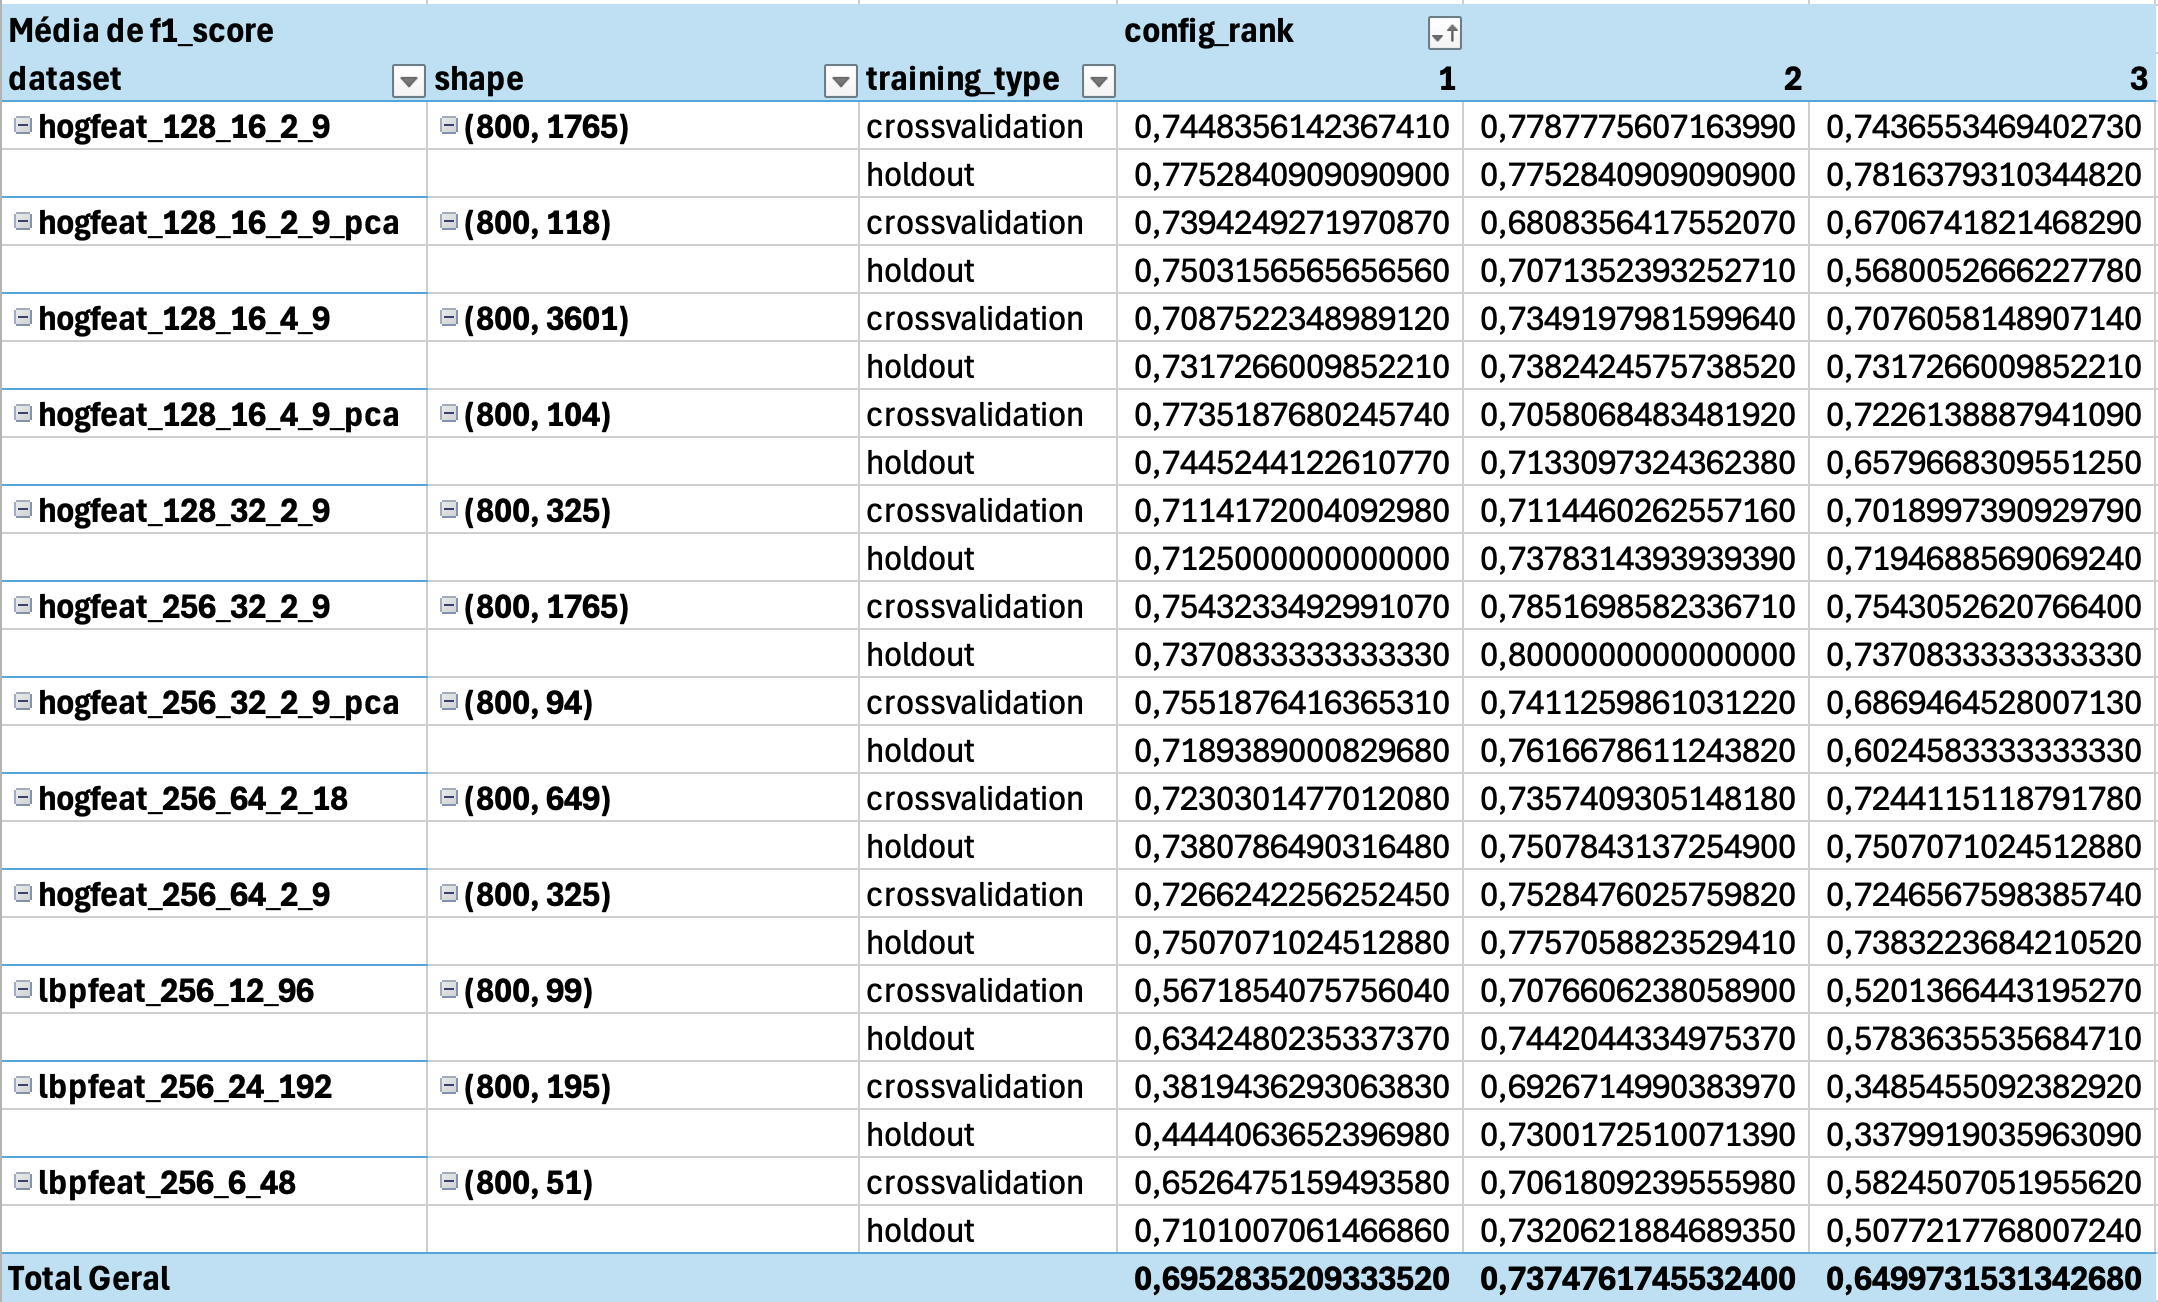
\includegraphics[width=\linewidth,height=\textheight,keepaspectratio]{tabelas/nb-matrix.png}

\vspace{0.5em}
\footnotesize
\textbf{Legenda:} cada coluna representa uma variação do algoritmo \textit{Naive Bayes}, e as linhas correspondem às diferentes bases avaliadas (descritores HOG e LBP, com ou sem PCA).
\end{table}

\vspace{1em}
\normalsize

\paragraph{Comportamento dos Parâmetros.}  
A média global de desempenho foi de aproximadamente 0{,}70, evidenciando um bom equilíbrio entre simplicidade e acurácia.  
O \texttt{GaussianNB} (Config. 2) obteve o melhor desempenho médio ($F1 = 0{,}737$), seguido pelo \texttt{ComplementNB} (Config. 1) com $F1 = 0{,}695$.  
O \texttt{MultinomialNB} apresentou o menor resultado médio ($F1 = 0{,}65$), indicando que o tratamento de atributos contínuos e normalizados se mostrou mais eficaz que a contagem discreta de frequências.  
Os tempos de execução foram baixos e estáveis (inferiores a 0{,}1 s), reforçando o baixo custo computacional do método.

\paragraph{Análise Estatística.}

O teste de Friedman resultou em $p = 0{,}0000057$, permitindo rejeitar a hipótese nula e confirmando diferenças estatisticamente significativas entre as três configurações.  
A Tabela~\ref{tab:nb-nemenyi} apresenta a matriz de comparação par a par obtida pelo teste de Nemenyi, onde se observa diferença significativa entre o \texttt{GaussianNB} e o \texttt{MultinomialNB} ($p < 0{,}001$), além de uma diferença marginal entre o \texttt{ComplementNB} e o \texttt{MultinomialNB} ($p \approx 0{,}03$).  
Esses resultados demonstram que a suposição de distribuição gaussiana é mais adequada aos descritores contínuos derivados de HOG e LBP utilizados neste estudo.

\begin{table}[H]
\centering
\caption{Matriz de comparação par a par do teste de Nemenyi para as três configurações de Naive Bayes.}
\label{tab:nb-nemenyi}
\vspace{0.5em}

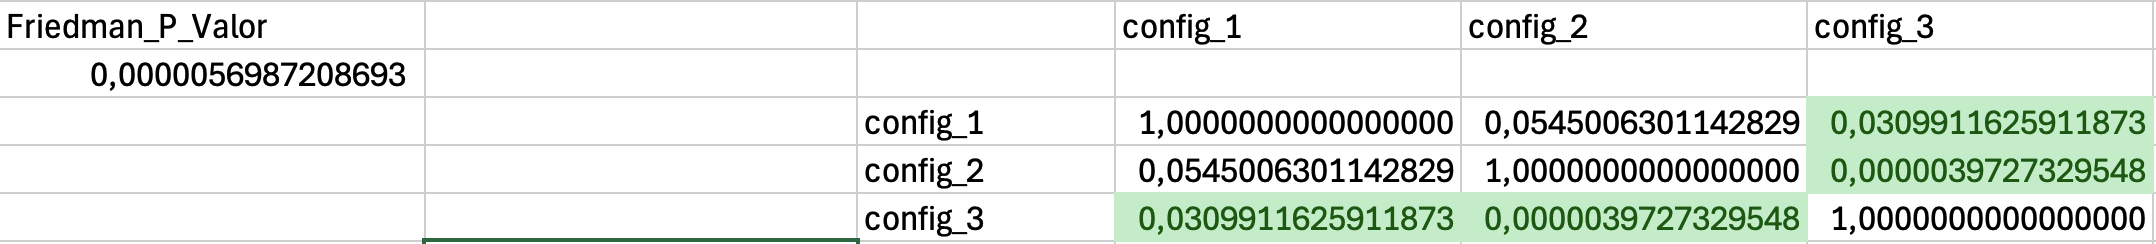
\includegraphics[width=\linewidth,height=\textheight,keepaspectratio]{tabelas/nb-statistic.png}

\vspace{0.5em}
\footnotesize
\textbf{Legenda:} células destacadas em verde indicam diferenças estatisticamente significativas ($p < 0{,}05$).  
O teste foi aplicado após rejeição da hipótese nula no teste de Friedman.
\end{table}

\vspace{1em}
\normalsize
\end{landscape}


\paragraph{Desempenho Global e Custo Computacional}

A Figura~\ref{fig:nb-rank} apresenta as médias de \textit{F1-score}, desvios padrão e tempos de execução das três configurações.  
O \texttt{GaussianNB} destacou-se como o modelo mais estável e eficiente, com desvio padrão de apenas 0{,}03 no \textit{F1-score}.  
As diferenças de tempo entre as variantes foram desprezíveis, mantendo a característica de extrema rapidez do método probabilístico, mesmo em bases de maior dimensionalidade.

\begin{figure}[H]
\centering
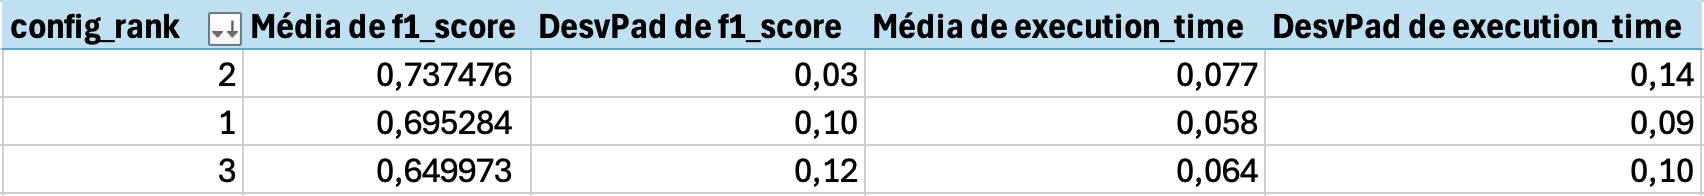
\includegraphics[width=0.9\linewidth]{tabelas/nb-rank.png}
\caption{Desempenho médio, desvio padrão e tempo de execução das três configurações do Naive Bayes.}
\label{fig:nb-rank}
\end{figure}


\paragraph{Interpretação dos Resultados}

Os resultados indicam clara vantagem do \texttt{GaussianNB} sobre as demais variantes, o que é consistente com a natureza contínua dos atributos extraídos pelos descritores HOG e LBP.  
O desempenho do \texttt{ComplementNB} foi intermediário, beneficiado por sua capacidade de ajustar probabilidades em situações de desbalanceamento de classes, enquanto o \texttt{MultinomialNB} mostrou-se menos adequado, possivelmente devido à ausência de variáveis categóricas genuínas.  
Em termos práticos, o Naive Bayes demonstrou excelente relação entre desempenho e custo, mantendo-se como um modelo probabilístico simples e eficiente.

\paragraph{Limitações e Observações}

Apesar da sua simplicidade e rapidez, o \textit{Naive Bayes} apresenta limitações relevantes neste contexto.  
Além da suposição de independência entre atributos, que reduz sua capacidade de capturar correlações entre pixels, o método é sensível à escala e ao sinal dos valores de entrada.  
Em particular, o \texttt{MultinomialNB} mostrou incompatibilidade com as bases reduzidas por PCA, que incluem componentes com valores negativos, exigindo reescalonamento prévio para que o modelo funcione corretamente.  
Essas restrições limitaram sua aplicabilidade em cenários híbridos com outros classificadores.


\subsubsection{Perceptron Multicamadas (MLP)}

Os experimentos com o \textit{Multi-Layer Perceptron} (MLP) buscaram analisar o impacto da arquitetura da rede, da função de ativação e da taxa de aprendizado sobre o desempenho de classificação. Foram testadas dez configurações, variando o número de camadas ocultas, o tamanho dos neurônios em cada camada, as funções de ativação (\texttt{relu}, \texttt{tanh}, \texttt{logistic}, \texttt{identity}), o otimizador (\texttt{adam} ou \texttt{sgd}) e o número máximo de iterações.

A Tabela~\ref{tab:mlp-config} apresenta as configurações avaliadas no experimento.

\begin{table}[H]
\centering
\caption{Configurações avaliadas para o classificador MLP.}
\label{tab:mlp-config}
\begin{tabularx}{\textwidth}{@{}>{\centering\arraybackslash}p{0.9cm} >{\ttfamily\raggedright\arraybackslash}X@{}}
\toprule
\textbf{Config.} & \textbf{Parâmetros} \\
\midrule
1 & \{activation: relu, hidden\_layer\_sizes: (200, 100), learning\_rate\_init: 0.005, max\_iter: 500, solver: adam\} \\
2 & \{activation: logistic, hidden\_layer\_sizes: (200, 100, 50), learning\_rate\_init: 0.005, max\_iter: 500, solver: adam\} \\
3 & \{activation: relu, hidden\_layer\_sizes: 50, learning\_rate\_init: 0.01, max\_iter: 500, solver: adam\} \\
4 & \{activation: tanh, hidden\_layer\_sizes: (150, 75), learning\_rate\_init: 0.01, max\_iter: 500, solver: adam\} \\
5 & \{activation: relu, hidden\_layer\_sizes: (200, 100), learning\_rate\_init: 0.01, max\_iter: 500, solver: adam\} \\
6 & \{activation: relu, hidden\_layer\_sizes: (200, 100, 50), learning\_rate\_init: 0.01, max\_iter: 500, solver: sgd\} \\
7 & \{activation: identity, hidden\_layer\_sizes: (200, 100, 50), learning\_rate\_init: 0.001, max\_iter: 500, solver: adam\} \\
8 & \{activation: relu, hidden\_layer\_sizes: (200, 100, 50), learning\_rate\_init: 0.005, max\_iter: 500, solver: adam\} \\
9 & \{activation: relu, hidden\_layer\_sizes: (150, 100), learning\_rate\_init: 0.01, max\_iter: 500, solver: adam\} \\
10 & \{activation: relu, hidden\_layer\_sizes: (200, 100), learning\_rate\_init: 0.001, max\_iter: 1500, solver: adam\} \\
\bottomrule
\end{tabularx}
\end{table}



\begin{landscape}
\begin{table}[H]
\centering
\caption{Médias de \textit{F1-score} por configuração e base de dados para o classificador MLP.}
\label{tab:mlp-matrix}
\vspace{0.5em}

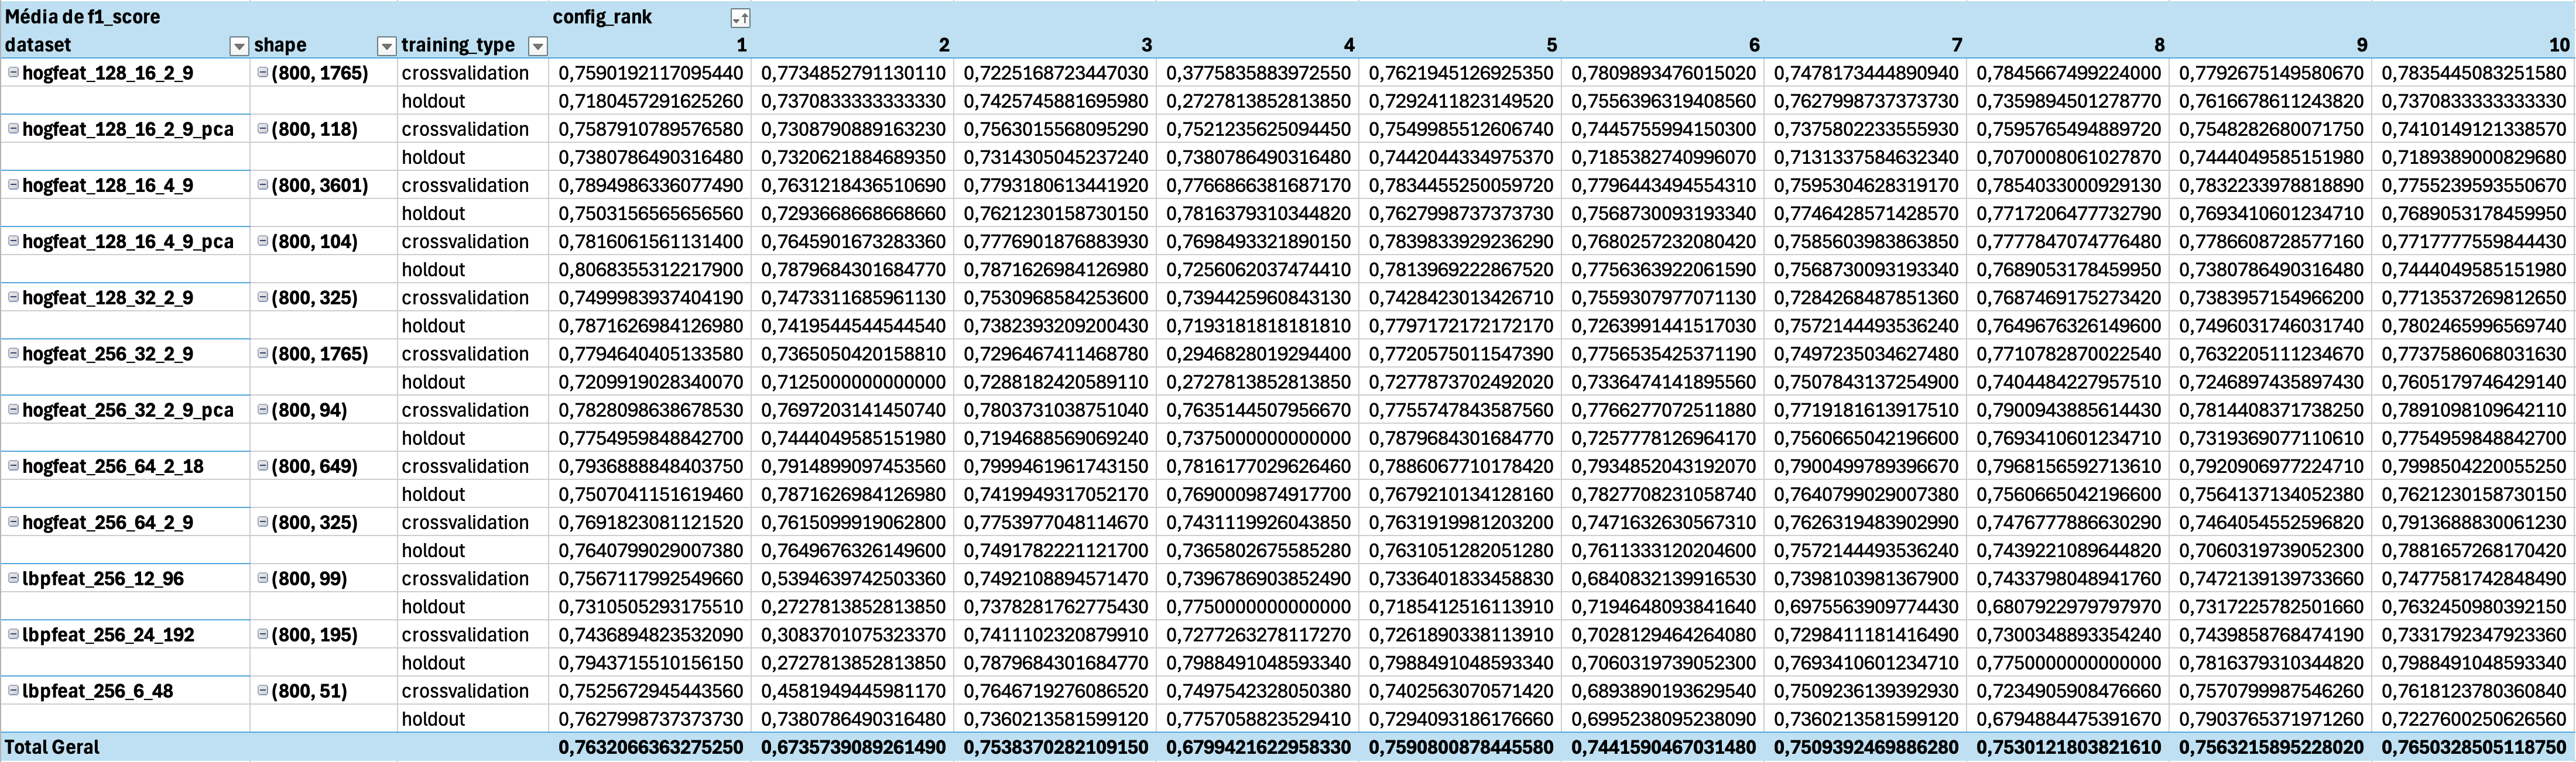
\includegraphics[width=\linewidth,height=\textheight,keepaspectratio]{tabelas/mlp-matrix.png}

\vspace{0.5em}
\footnotesize
\textbf{Legenda:} cada coluna representa uma configuração distinta de arquitetura e parâmetros de treinamento;  
as linhas correspondem às diferentes bases avaliadas (descritores HOG e LBP, com ou sem PCA).
\end{table}

\vspace{1em}
\normalsize

\paragraph{Comportamento dos Parâmetros.}  
A média global de desempenho foi de aproximadamente 0{,}76, o maior valor entre os classificadores individuais.  
As melhores configurações (1, 5, 9 e 10) utilizaram a função de ativação \texttt{relu} e arquiteturas com duas ou três camadas ocultas, evidenciando a capacidade dessa função em capturar padrões não lineares mais complexos.  
Configurações com \texttt{tanh} ou \texttt{logistic} obtiveram resultados inferiores, sugerindo que as funções saturadas limitaram o aprendizado em bases com alta dimensionalidade.  
Modelos mais profundos ou com maior número de iterações (como a Config. 10, com \texttt{max\_iter}=1500) atingiram o melhor \textit{F1-score} ($\approx 0{,}765$ ), ao custo de maior tempo médio de execução ($\approx  13 s$) e variância considerável.
\end{landscape}



\begin{landscape}

\paragraph{Influência do Tipo de Descritor e Validação}

O desempenho foi consistentemente superior nas bases HOG, com valores acima de 0{,}78 em média, enquanto as LBP permaneceram ligeiramente abaixo de 0{,}75.  
As versões reduzidas por PCA mantiveram resultados comparáveis, o que indica que a compressão das representações não prejudicou a aprendizagem das redes neurais.  
O protocolo de \textit{cross-validation} produziu maior estabilidade e menor dispersão nos resultados, reforçando a capacidade de generalização das configurações avaliadas.

\begin{table}[H]
\centering
\caption{Matriz de comparação par a par do teste de Nemenyi para as dez configurações do MLP.}
\label{tab:mlp-nemenyi}
\vspace{0.5em}

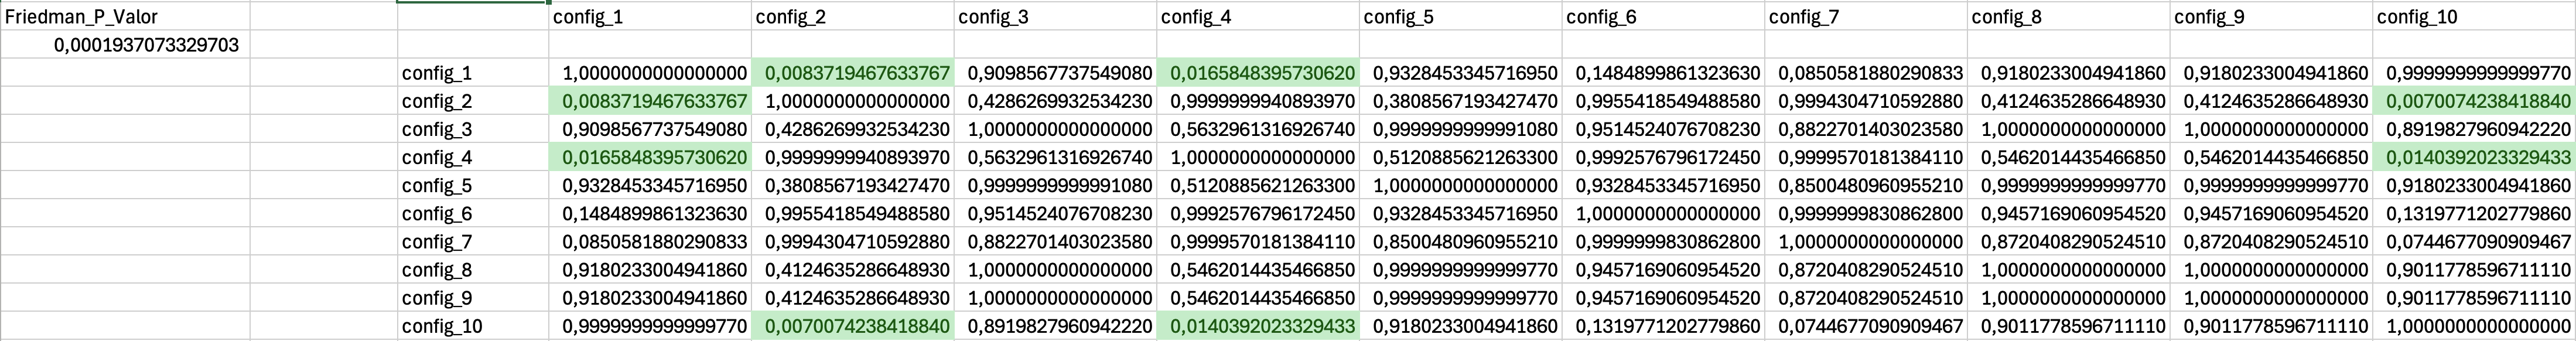
\includegraphics[width=\linewidth,height=\textheight,keepaspectratio]{tabelas/mlp-statistic.png}

\vspace{0.5em}
\footnotesize
\textbf{Legenda:} cada célula apresenta o valor-$p$ da comparação entre duas configurações;  
células destacadas em verde indicam diferenças estatisticamente significativas ($p < 0{,}05$).  
O teste foi aplicado após rejeição da hipótese nula no teste de Friedman.
\end{table}

\vspace{1em}
\normalsize

\paragraph{Análise Estatística.}  
O teste de Friedman resultou em $p = 0{,}00019$, confirmando diferenças estatisticamente significativas entre as dez configurações avaliadas.  
A matriz de Nemenyi, apresentada na Tabela~\ref{tab:mlp-nemenyi}, evidencia que as configurações 1, 5, 9 e 10 apresentaram desempenho significativamente superior em relação às demais, especialmente quando comparadas às configurações 2 e 4, cujos valores-$p$ ficaram abaixo de 0{,}05.  
Essas configurações de destaque compartilham o uso da função de ativação \texttt{relu} e arquiteturas com duas ou mais camadas ocultas, demonstrando que a profundidade moderada e o uso de funções de ativação não saturadas foram determinantes para o melhor desempenho do MLP.  
Os resultados confirmam a influência significativa da escolha da arquitetura e dos hiperparâmetros sobre o desempenho final, evidenciando que redes mais rasas ou com funções saturadas (\texttt{tanh} e \texttt{logistic}) tendem a ter capacidade discriminativa reduzida neste conjunto de dados.

\end{landscape}


\paragraph{Desempenho Global e Custo Computacional}

A Figura~\ref{fig:mlp-rank} resume as médias de \textit{F1-score}, desvios padrão e tempos de execução.  
Os tempos médios variaram entre 4 e 14 s, com desvio padrão elevado nas execuções mais longas devido à diferença de convergência entre bases de alta e baixa dimensionalidade.  
Apesar disso, as redes com \texttt{relu} apresentaram convergência consistente, com desvios médios de apenas 0{,}02 no \textit{F1-score}, sugerindo estabilidade e eficiência na otimização com \texttt{adam}.

\begin{figure}[H]
\centering
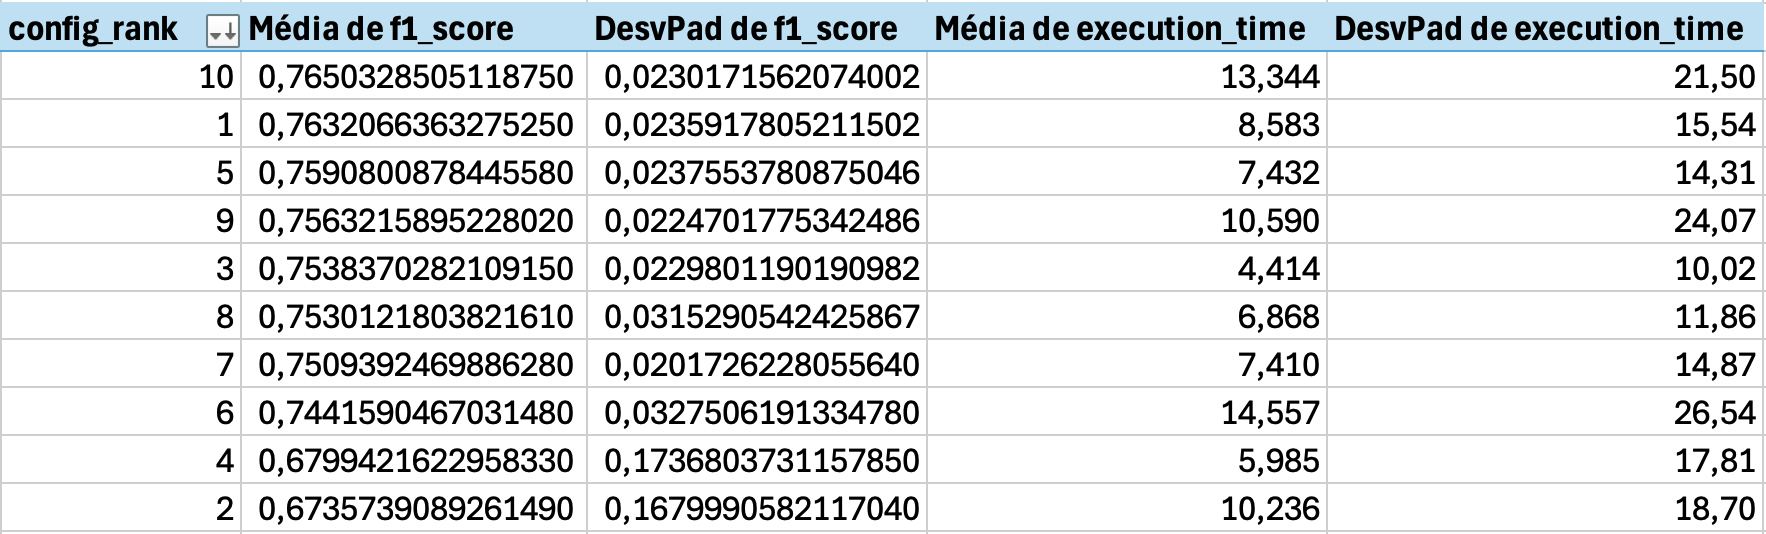
\includegraphics[width=0.9\linewidth]{tabelas/mlp-rank.png}
\caption{Desempenho médio, desvio padrão e tempo de execução das dez configurações do MLP.}
\label{fig:mlp-rank}
\end{figure}

\paragraph{Interpretação dos Resultados}

A Rede Neural Multicamadas apresentou desempenho superior aos demais classificadores individuais, confirmando sua capacidade de modelar relações complexas entre as variáveis.  
O destaque das funções \texttt{relu} e \texttt{adam} evidencia o bom equilíbrio entre rapidez de convergência e generalização.  
As diferenças significativas encontradas indicam que a arquitetura e o número de iterações influenciam diretamente o desempenho final, sendo necessário ajustar esses parâmetros conforme a dimensionalidade da base.  
A combinação de múltiplas camadas e taxas de aprendizado moderadas mostrou-se particularmente eficiente em bases HOG de maior dimensão.

\paragraph{Limitações e Observações}

Apesar do desempenho elevado, o custo computacional foi o mais alto entre os classificadores testados.  
Modelos mais complexos apresentaram grande variabilidade no tempo de treinamento e risco de sobreajuste em bases pequenas.  
Além disso, a sensibilidade à inicialização e ao número de iterações pode causar divergências de convergência entre execuções.  
Ainda assim, o MLP destacou-se como o modelo mais robusto e expressivo do conjunto, servindo como referência para comparação com os comitês de classificadores.

\subsubsection{Síntese Comparativa entre Classificadores Individuais}

\paragraph{Comparação dos Melhores Resultados.}
A Tabela~\ref{tab:top1-matrix} apresenta as médias de \textit{F1-score} obtidas pelas melhores configurações de cada classificador — \texttt{KNN Config 2}, \texttt{DTree Config 8}, \texttt{NB Config 2} e \texttt{MLP Config 10} — sobre as 12 bases de dados selecionadas (seis variantes de HOG e três de LBP, cada uma avaliada com dois protocolos de validação).  

\begin{landscape}
\begin{table}[H]
\centering
\caption{Desempenho das melhores configurações de cada classificador em todas as bases avaliadas.}
\label{tab:top1-matrix}
\vspace{0.5em}

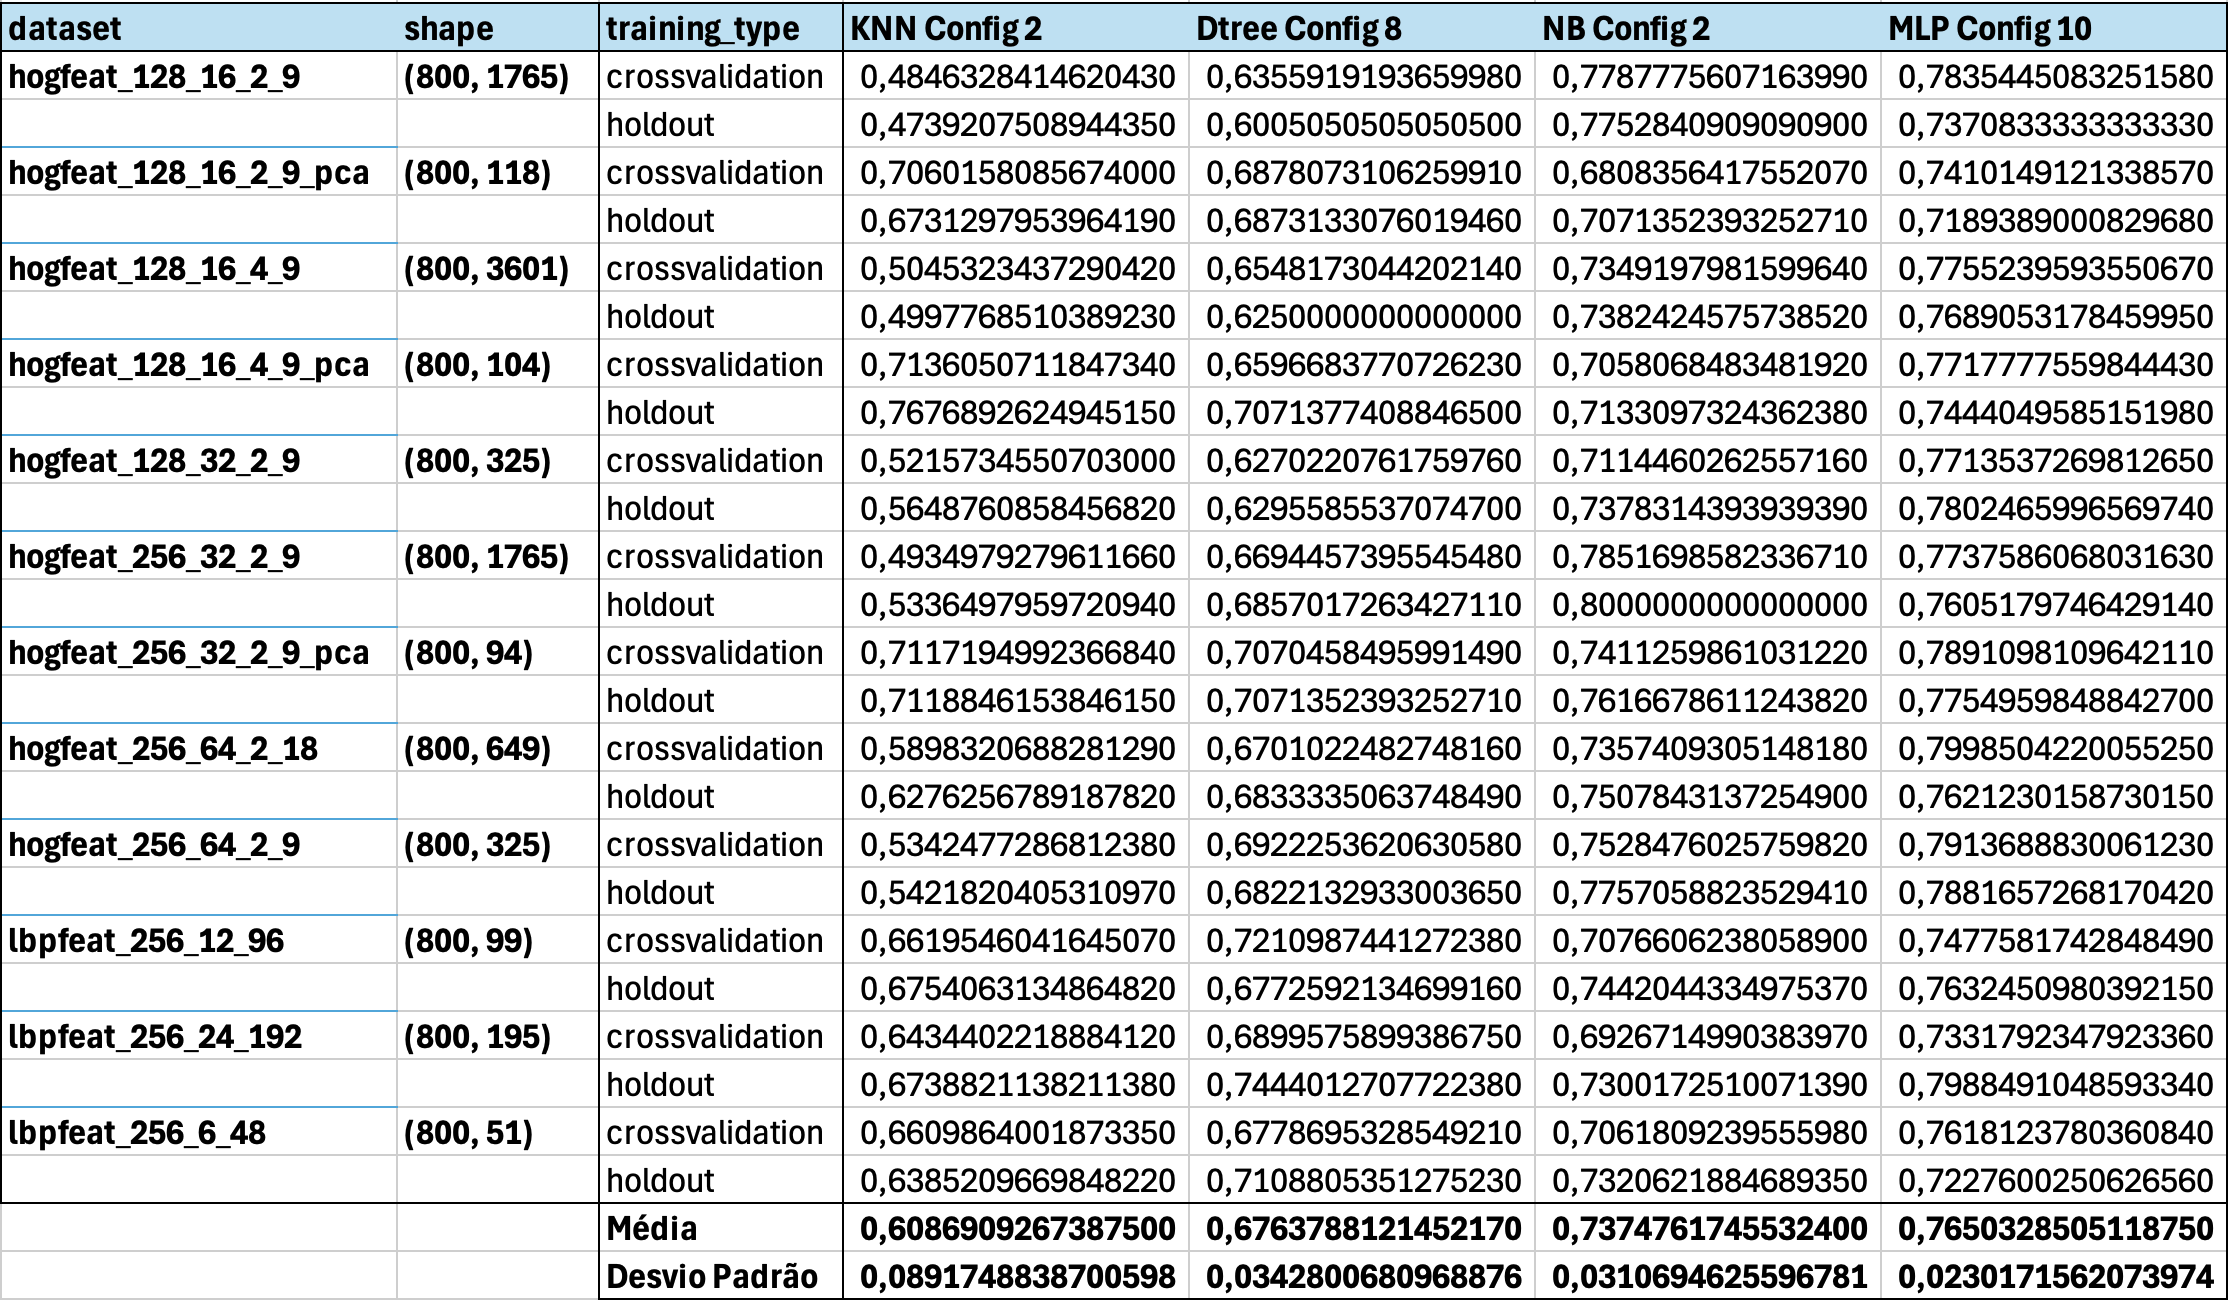
\includegraphics[width=\linewidth,height=\textheight,keepaspectratio]{tabelas/top1-matrix.png}

\vspace{0.5em}
\footnotesize
\textbf{Legenda:} cada coluna representa a melhor configuração de cada modelo; as linhas correspondem às bases de dados avaliadas.
\end{table}
\end{landscape}

O \textit{MLP} apresentou o maior desempenho médio (\(0{,}765\)), seguido pelo \textit{Naive Bayes} (\(0{,}737\)), pela Árvore de Decisão (\(0{,}676\)) e pelo \textit{k}-NN (\(0{,}609\)).  
A diferença entre o melhor e o pior modelo ultrapassa 0{,}15 em média, o que demonstra impacto expressivo da escolha do classificador sobre a capacidade discriminativa.  
Os desvios-padrão revelam estabilidade considerável do MLP e do k-NN, enquanto o Naive Bayes apresentou variação moderada, possivelmente influenciada pela suposição de independência entre atributos.  

\vspace{1em}

\paragraph{Análise Estatística Conjunta (Friedman e Nemenyi).}
O teste de Friedman foi aplicado às médias de \textit{F1-score} dos quatro classificadores sobre as 24 execuções (12 bases × 2 protocolos), resultando em \( \chi^2_F = 49{,}65 \) e \(p = 9{,}48 \times 10^{-11}\).  
Esse resultado indica diferenças estatisticamente significativas entre os classificadores (\(p < 0{,}001\)).  

A matriz de comparações par a par do teste de Nemenyi é apresentada na Tabela~\ref{tab:top1-statistic}.  
As diferenças mais acentuadas ocorreram entre o MLP e os demais modelos, todas com \(p < 0{,}001\), evidenciando que a rede neural multicamadas superou de forma consistente as abordagens baseadas em instâncias e árvores.  
A diferença entre k-NN e Árvore de Decisão, por outro lado, não foi estatisticamente significativa (\(p = 0{,}149\)).

\begin{landscape}
\begin{table}[H]
\centering
\caption{Matriz de comparação par a par do teste de Nemenyi entre os quatro classificadores individuais.}
\label{tab:top1-statistic}
\vspace{0.5em}

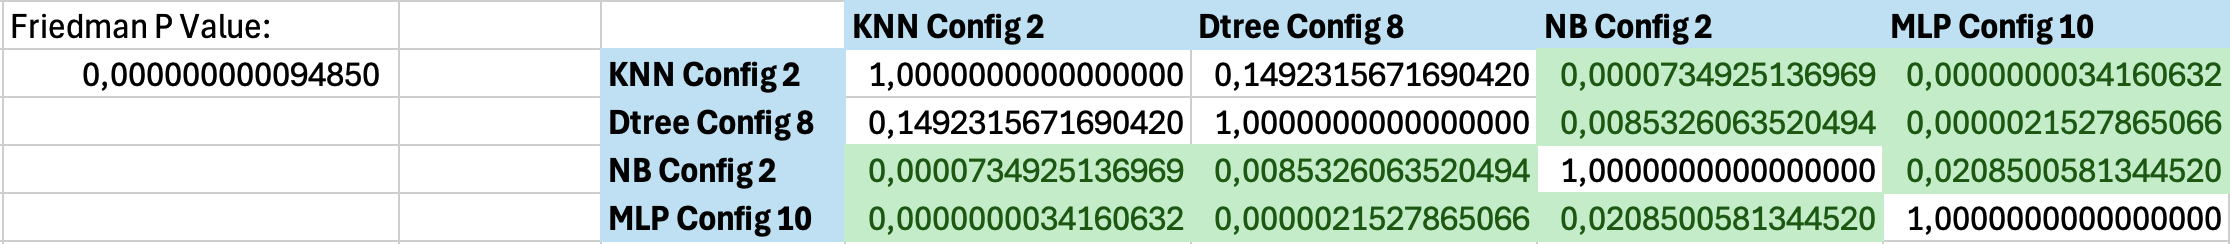
\includegraphics[width=\linewidth,height=\textheight,keepaspectratio]{tabelas/top1-statistic.png}

\vspace{0.5em}
\footnotesize
\textbf{Legenda:} cada célula indica o valor-$p$ da comparação entre dois modelos; células destacadas em verde correspondem a diferenças estatisticamente significativas (\(p < 0{,}05\)).
\end{table}
\end{landscape}

\vspace{1em}
\paragraph{Discussão sobre Generalização e Custo Computacional.}
O MLP destacou-se não apenas em desempenho, mas também em estabilidade, apresentando o menor desvio relativo entre bases de alta e baixa dimensionalidade.  
O Naive Bayes, embora estatisticamente inferior, apresentou custo computacional muito baixo e consistência entre protocolos de validação, o que o torna competitivo para aplicações com restrição de recursos.  
A Árvore de Decisão manteve desempenho intermediário, oferecendo boa interpretabilidade e tempo de treinamento reduzido.  
Por outro lado, o k-NN apresentou desempenho inferior nas bases de maior dimensão, refletindo a sensibilidade da métrica de distância ao aumento de atributos.  

Em síntese, os resultados indicam que o \textit{MLP Config 10} foi o modelo com melhor capacidade de generalização, enquanto o \textit{Naive Bayes Config 2} destacou-se como alternativa eficiente e de baixo custo.  
A superioridade estatística do MLP, confirmada pelos testes de Friedman e Nemenyi, justifica seu uso como referência nas análises subsequentes de comitês de classificadores.






\subsubsection{Bagging}

O método \textit{Bootstrap Aggregating} (Bagging) foi avaliado com o objetivo de mensurar o impacto da agregação de estimadores homogêneos sobre o desempenho e a estabilidade dos modelos.  
Foram testadas doze configurações, combinando quatro classificadores base (\texttt{KNN}, \texttt{DecisionTree}, \texttt{Naive Bayes} e \texttt{MLP}) e três quantidades de estimadores (\texttt{n\_estimators} = 10, 20, 30).  
A Tabela~\ref{tab:bagging-config} apresenta as configurações avaliadas.

\begin{table}[H]
\centering
\caption{Configurações avaliadas para o método Bagging.}
\label{tab:bagging-config}
\begin{tabularx}{\textwidth}{@{}>{\centering\arraybackslash}p{0.9cm} >{\ttfamily\raggedright\arraybackslash}X@{}}
\toprule
\textbf{Config.} & \textbf{Parâmetros} \\
\midrule
1 & \{estimatorModel: 'knn', n\_estimators: 10\} \\
2 & \{estimatorModel: 'knn', n\_estimators: 20\} \\
3 & \{estimatorModel: 'knn', n\_estimators: 30\} \\
4 & \{estimatorModel: 'dtree', n\_estimators: 10\} \\
5 & \{estimatorModel: 'dtree', n\_estimators: 20\} \\
6 & \{estimatorModel: 'dtree', n\_estimators: 30\} \\
7 & \{estimatorModel: 'nb', n\_estimators: 10\} \\
8 & \{estimatorModel: 'nb', n\_estimators: 20\} \\
9 & \{estimatorModel: 'nb', n\_estimators: 30\} \\
10 & \{estimatorModel: 'mlp', n\_estimators: 10\} \\
11 & \{estimatorModel: 'mlp', n\_estimators: 20\} \\
12 & \{estimatorModel: 'mlp', n\_estimators: 30\} \\
\bottomrule
\end{tabularx}
\end{table}


\begin{landscape}
\begin{table}[H]
\centering
\caption{Médias de \textit{F1-score} por configuração e base de dados para o método Bagging.}
\label{tab:bagging-matrix}
\vspace{0.5em}

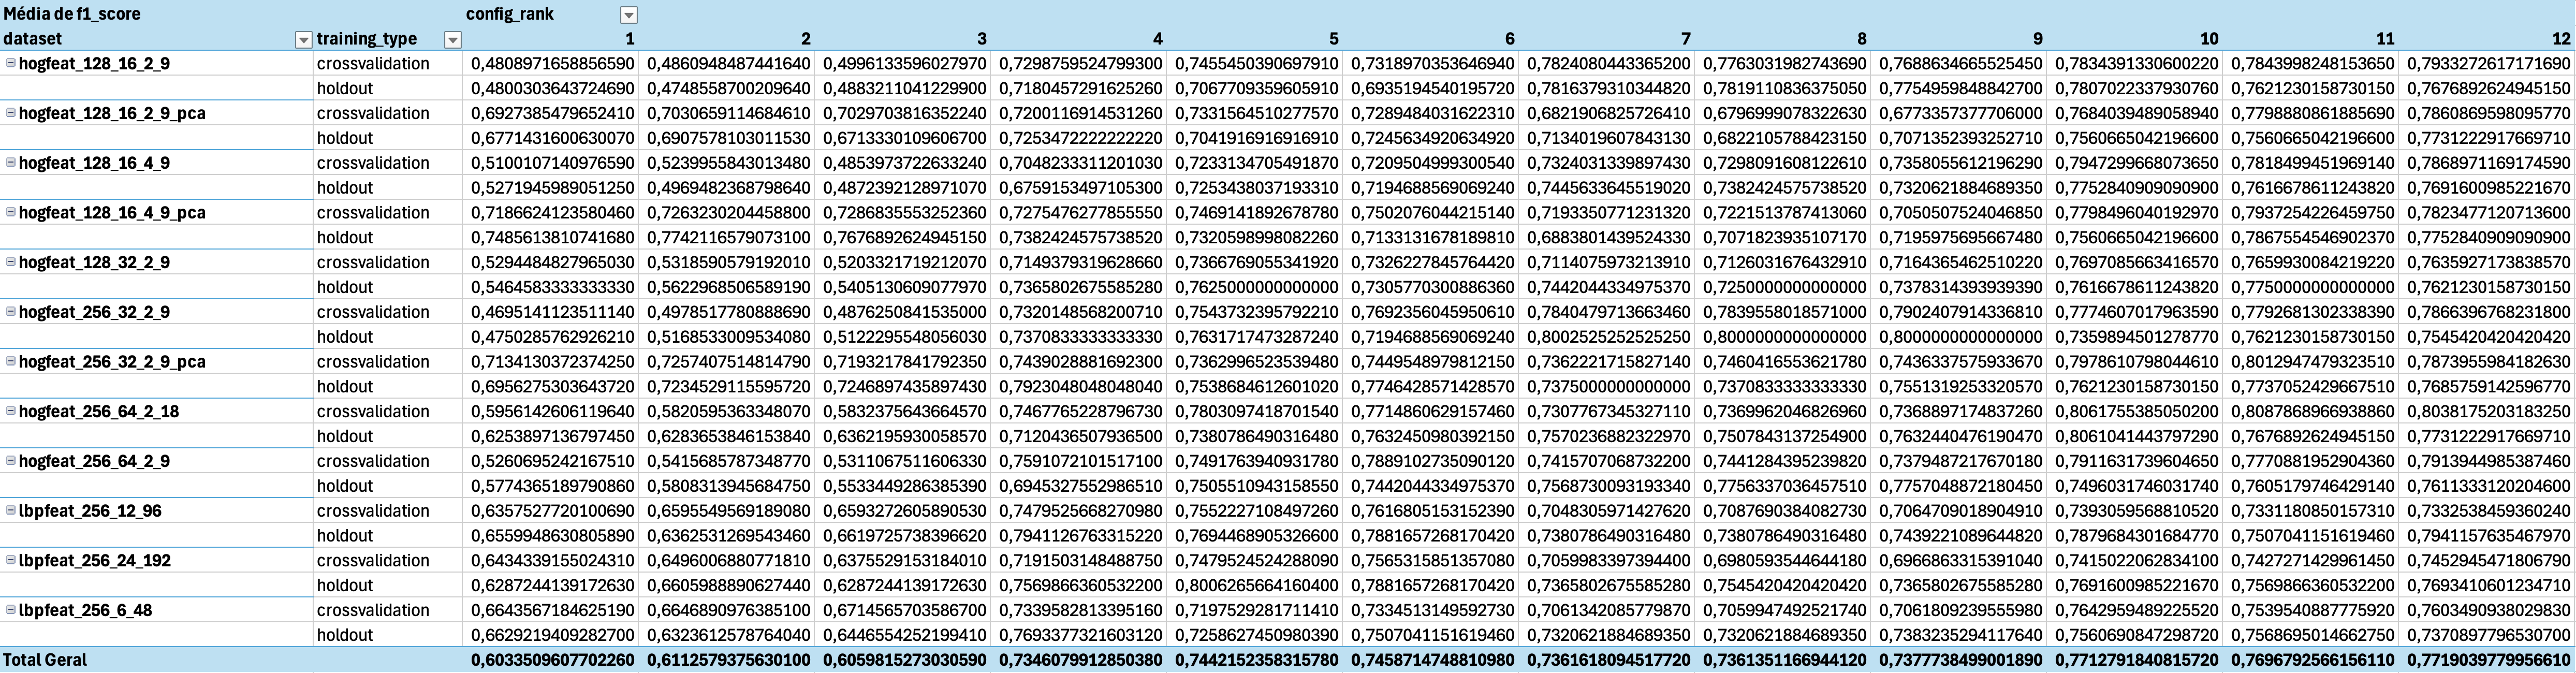
\includegraphics[width=\linewidth,height=\textheight,keepaspectratio]{tabelas/Bagging-matrix.png}

\vspace{0.5em}
\footnotesize
\textbf{Legenda:} cada coluna representa uma configuração distinta de estimador e número de modelos agregados;  
as linhas correspondem às diferentes bases avaliadas (descritores HOG e LBP, com ou sem PCA).
\end{table}

\vspace{1em}
\normalsize


\paragraph{Comportamento dos Parâmetros.}  
A média global de desempenho foi de aproximadamente \(0{,}714\), superando todos os classificadores individuais exceto o MLP.  
Os comitês baseados em redes neurais (\texttt{MLP}, Configs 10–12) obtiveram as maiores médias de \textit{F1-score}, entre \(0{,}769\) e \(0{,}772\), com baixos desvios-padrão (\(\approx 0{,}019\)), indicando estabilidade elevada.  
Entre os modelos de menor complexidade, o Bagging com Árvores de Decisão (\texttt{DecisionTree}, Configs 4–6) apresentou o maior ganho relativo, com médias próximas de \(0{,}745\), superando em quase \(+0{,}07\) o desempenho da árvore individual.  
Os ensembles de \texttt{Naive Bayes} mantiveram resultados semelhantes aos modelos originais (\(0{,}737 \rightarrow 0{,}736\)–\(0{,}738\)), enquanto os com \texttt{KNN} tiveram leve queda, refletindo a estabilidade inerente ao método.

Ao comparar cada estimador com seu equivalente individual:
\begin{itemize}
    \item O \texttt{KNN} apresentou leve redução — o melhor ensemble (\(0{,}611\)) foi equivalente ou inferior ao modelo individual (\(0{,}609\)), mostrando que o Bagging não é vantajoso para estimadores já estáveis.
    \item O \texttt{DecisionTree} teve o maior ganho proporcional, com melhora média de \(0{,}676 \rightarrow 0{,}745\), confirmando que a agregação reduz a variância de modelos instáveis.
    \item O \texttt{Naive Bayes} manteve desempenho quase idêntico ao individual, sem ganhos relevantes.
    \item O \texttt{MLP} obteve o melhor resultado absoluto (\(0{,}772\)), mas com ganho marginal frente à versão individual (\(0{,}765\)), indicando que o Bagging atuou principalmente reduzindo variação, e não ampliando desempenho.
\end{itemize}

Esses resultados indicam que o Bagging é mais eficaz em estimadores de alta variância (como Árvores de Decisão), enquanto seus efeitos sobre modelos de alta estabilidade (KNN, NB) ou baixo viés (MLP) tendem a ser marginais.

\end{landscape}


\begin{landscape}

\paragraph{Análise Estatística.}
O teste de Friedman resultou em \( \chi^2_F = 110{,}84 \) e \( p = 4{,}1 \times 10^{-17} \), evidenciando diferenças altamente significativas entre as doze configurações avaliadas.  
A matriz de comparações par a par do teste de Nemenyi, apresentada na Tabela~\ref{tab:bagging-statistic}, confirma que as configurações com \texttt{MLP} (10–12) apresentaram desempenho estatisticamente superior às demais (\(p < 0{,}001\)).  
As diferenças entre os conjuntos baseados em \texttt{DecisionTree} e \texttt{Naive Bayes} também foram significativas frente às versões com \texttt{KNN}, reforçando o papel do estimador base na eficácia do comitê.

\begin{table}[H]
\centering
\caption{Matriz de comparação par a par do teste de Nemenyi para as doze configurações do Bagging.}
\label{tab:bagging-statistic}
\vspace{0.5em}

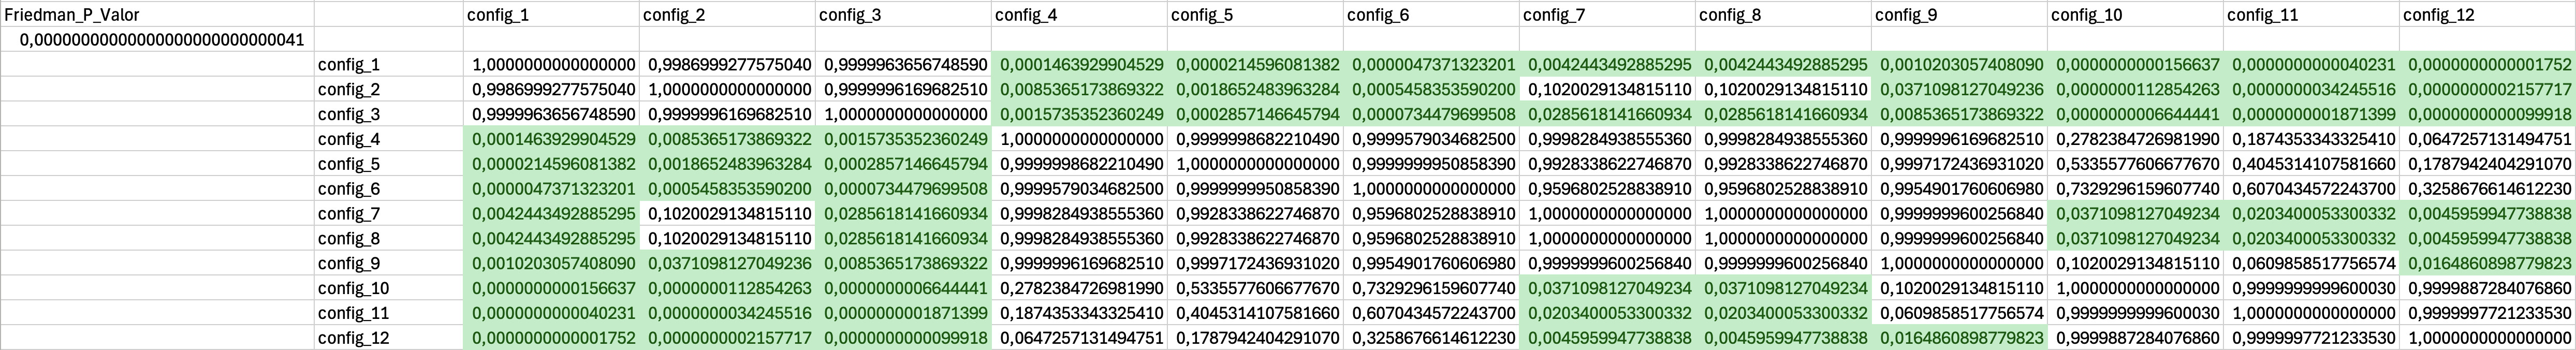
\includegraphics[width=\linewidth,height=\textheight,keepaspectratio]{tabelas/Bagging-statistic.png}

\vspace{0.5em}
\footnotesize
\textbf{Legenda:} cada célula apresenta o valor-$p$ da comparação entre duas configurações;  
as células destacadas em verde indicam diferenças estatisticamente significativas (\(p < 0{,}05\)).  
O teste de Nemenyi foi aplicado após rejeição da hipótese nula no teste de Friedman.
\end{table}

\vspace{1em}
\normalsize
\end{landscape}


\paragraph{Desempenho Global e Custo Computacional.}
A Figura~\ref{fig:bagging-rank} resume as médias de \textit{F1-score}, desvios-padrão e tempos de execução.  
Os custos computacionais variaram amplamente entre os estimadores:  
os comitês baseados em \texttt{KNN} e \texttt{DecisionTree} tiveram tempos inferiores a 5 s, enquanto os com \texttt{MLP} atingiram até 177 s, devido à sobrecarga de treinamento de múltiplas redes.  
Ainda assim, as configurações com MLP exibiram boa relação entre desempenho e estabilidade, com desvios médios abaixo de 0{,}02, mas custo até 30 vezes superior ao dos demais modelos.

\begin{figure}[H]
\centering
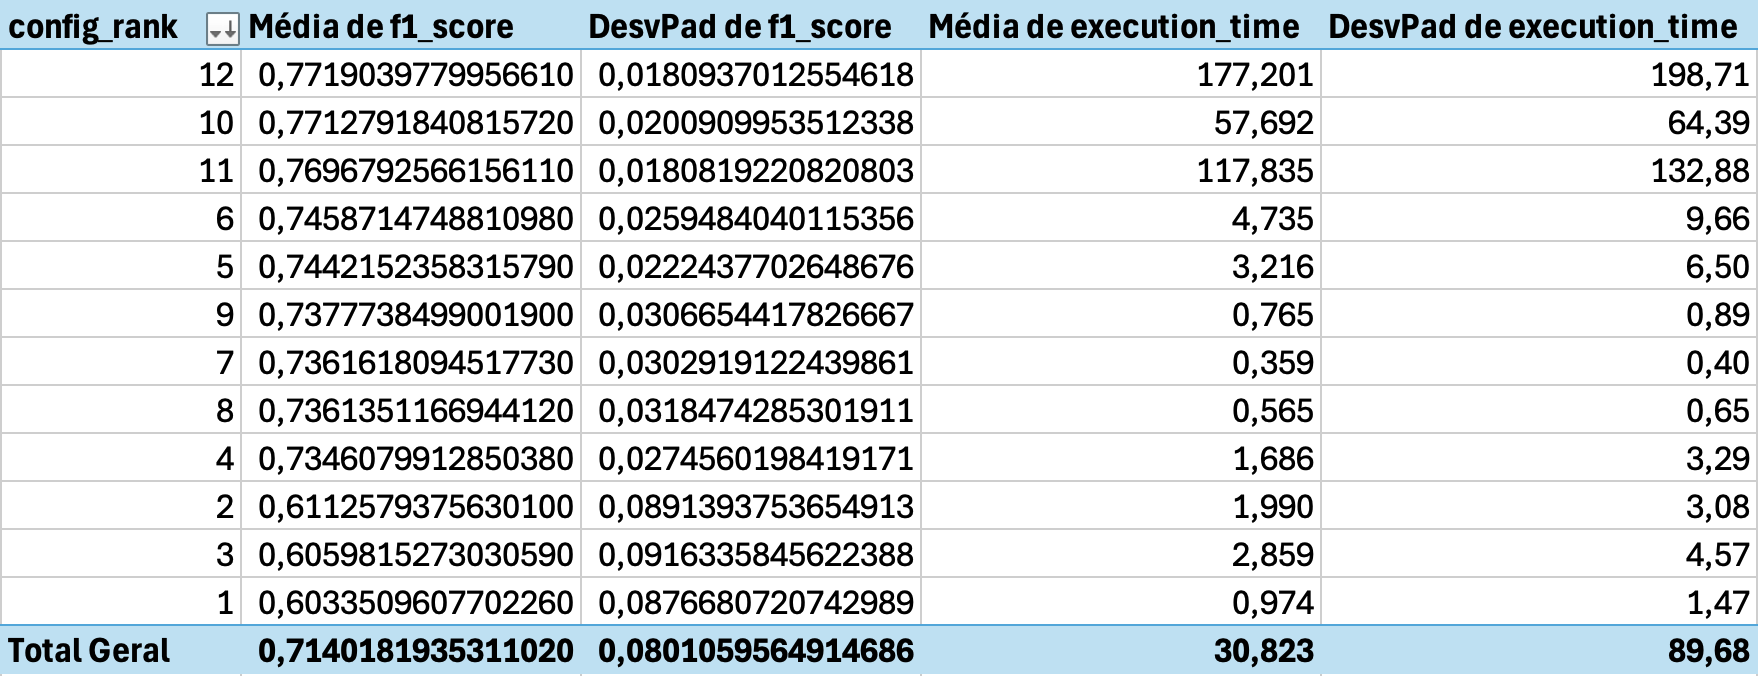
\includegraphics[width=0.9\linewidth]{tabelas/Bagging-rank.png}
\caption{Desempenho médio, desvio padrão e tempo de execução das doze configurações do Bagging.}
\label{fig:bagging-rank}
\end{figure}


\paragraph{Interpretação dos Resultados.}
Os resultados indicam que o Bagging melhora substancialmente o desempenho de classificadores instáveis, como as Árvores de Decisão, e estabiliza o comportamento de modelos de maior complexidade, como o MLP.  
Entretanto, os ganhos marginais observados nos modelos já estáveis (KNN e Naive Bayes) sugerem que o método não é igualmente eficaz em todos os contextos.  
Assim, o efeito predominante do Bagging neste conjunto foi a redução da variância, mais do que o aumento absoluto do desempenho médio.

\paragraph{Limitações e Observações.}
Embora os ensembles com MLP tenham alcançado as maiores médias de \textit{F1-score}, apresentaram também o maior custo computacional e maior variabilidade de tempo entre execuções.  
Já os ensembles de DecisionTree confirmaram o comportamento clássico do Bagging, com ganhos consistentes e baixo custo adicional.  
De modo geral, o Bagging se mostrou uma estratégia eficaz de estabilização, especialmente para modelos sensíveis à variância, servindo como base de comparação para os comitês heterogêneos apresentados nas próximas seções.





\subsubsection{Random Forest}

O algoritmo \textit{Random Forest} foi avaliado para investigar o efeito da aleatorização de atributos e da quantidade de árvores sobre o desempenho global e a estabilidade do comitê.  
Foram testadas doze configurações, combinando três critérios de impureza (\texttt{gini}, \texttt{entropy} e \texttt{log\_loss}) com quatro tamanhos de floresta (\texttt{n\_estimators} = 10, 20, 30, 100).  
A Tabela~\ref{tab:rf-config} apresenta os parâmetros avaliados.

\begin{table}[H]
\centering
\caption{Configurações avaliadas para o classificador Random Forest.}
\label{tab:rf-config}
\begin{tabularx}{\textwidth}{@{}>{\centering\arraybackslash}p{0.9cm} >{\ttfamily\raggedright\arraybackslash}X@{}}
\toprule
\textbf{Config.} & \textbf{Parâmetros} \\
\midrule
1 & \{criterion: 'gini', n\_estimators: 10\} \\
2 & \{criterion: 'gini', n\_estimators: 20\} \\
3 & \{criterion: 'gini', n\_estimators: 30\} \\
4 & \{criterion: 'gini', n\_estimators: 100\} \\
5 & \{criterion: 'entropy', n\_estimators: 10\} \\
6 & \{criterion: 'entropy', n\_estimators: 20\} \\
7 & \{criterion: 'entropy', n\_estimators: 30\} \\
8 & \{criterion: 'entropy', n\_estimators: 100\} \\
9 & \{criterion: 'log\_loss', n\_estimators: 10\} \\
10 & \{criterion: 'log\_loss', n\_estimators: 20\} \\
11 & \{criterion: 'log\_loss', n\_estimators: 30\} \\
12 & \{criterion: 'log\_loss', n\_estimators: 100\} \\
\bottomrule
\end{tabularx}
\end{table}


\begin{landscape}
\begin{table}[H]
\centering
\caption{Médias de \textit{F1-score} por configuração e base de dados para o método Random Forest.}
\label{tab:rf-matrix}
\vspace{0.5em}

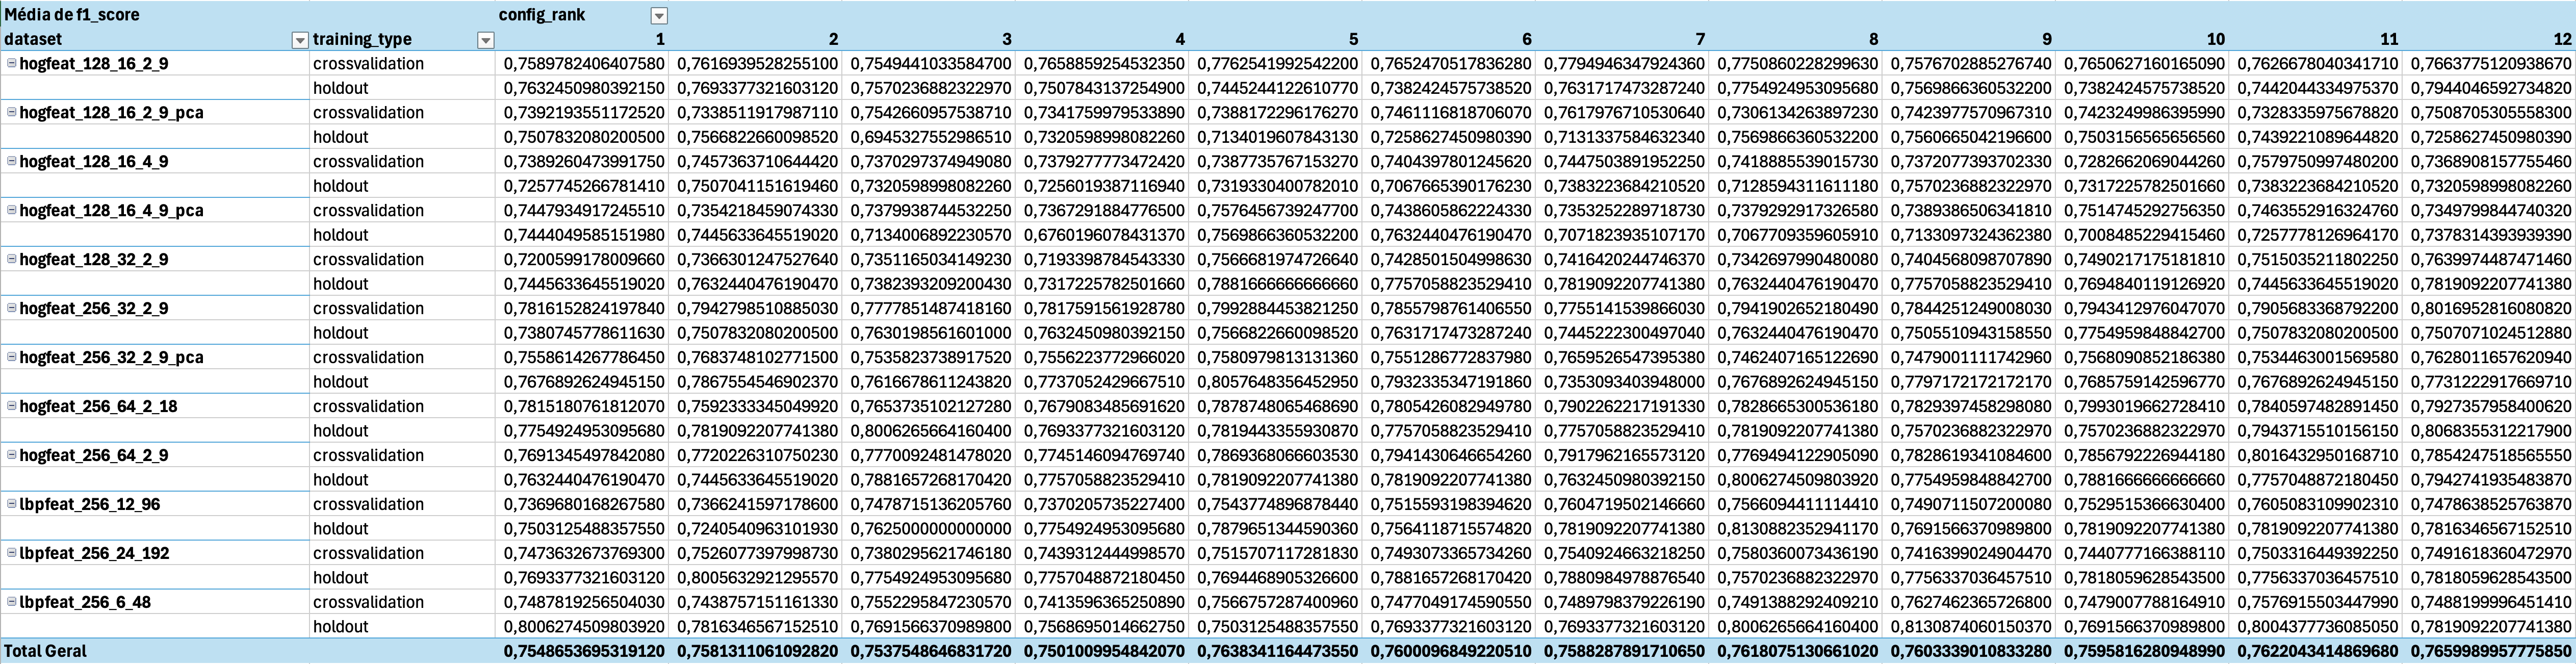
\includegraphics[width=\linewidth,height=\textheight,keepaspectratio]{tabelas/RandomForest-matrix.png}

\vspace{0.5em}
\footnotesize
\textbf{Legenda:} cada coluna representa uma configuração distinta do comitê, variando o critério de impureza e o número de árvores.
\end{table}

\vspace{1em}
\normalsize


\paragraph{Comportamento dos Parâmetros.}
O \textit{Random Forest} apresentou média global de \textit{F1-score} de \(0{,}759\), superior ao Bagging (\(0{,}714\)) e ao classificador individual de referência (\texttt{DecisionTree Config 8}, \(0{,}676\)).  
Os melhores resultados foram obtidos nas configurações 11 e 12 (critério \texttt{log\_loss}, 30 e 100 árvores), com médias de \(0{,}762\) e \(0{,}766\) respectivamente, e baixos desvios-padrão (\(\approx 0{,}021\)).  
Esses valores indicam que o aumento da diversidade — pela aleatorização de atributos — gerou ganhos expressivos de desempenho e estabilidade.

A variação do número de árvores revelou comportamento monotônico: as médias aumentaram gradualmente até 30 estimadores, estabilizando-se após esse ponto.  
O uso do critério \texttt{log\_loss} superou consistentemente \texttt{gini} e \texttt{entropy}, sugerindo melhor calibração probabilística em cenários com classes balanceadas.

Comparando com o classificador base e o comitê simples:
\begin{itemize}
    \item Frente à \texttt{DecisionTree} individual, o ganho médio foi de aproximadamente \( +0{,}08 \), confirmando a redução efetiva da variância e o aumento da robustez.
    \item Em relação ao \texttt{Bagging}, o acréscimo médio foi de \( +0{,}045 \), evidenciando o benefício adicional da aleatorização dos atributos na formação das árvores.
    \item O custo computacional manteve-se baixo ($\approx 1 s$ por modelo), sem variação relevante entre configurações.
\end{itemize}

\end{landscape}


\begin{landscape}
\paragraph{Análise Estatística.}
O teste de Friedman resultou em \( \chi^2_F = 27{,}73 \) e \( p = 9{,}76\times10^{-4} \), indicando diferenças estatisticamente significativas entre as doze configurações.  
A Tabela~\ref{tab:rf-statistic} apresenta os valores de \(p\) do teste de Nemenyi, revelando que as configurações com critério \texttt{log\_loss} (9–12) superaram significativamente as versões baseadas em \texttt{gini} (\(p < 0{,}05\)).  
As diferenças entre \texttt{entropy} e \texttt{log\_loss} foram menos acentuadas, sugerindo que o número de árvores exerce influência mais forte que o critério de impureza na consolidação do desempenho.

\begin{table}[H]
\centering
\caption{Matriz de comparação par a par do teste de Nemenyi para as doze configurações do Random Forest.}
\label{tab:rf-statistic}
\vspace{0.5em}

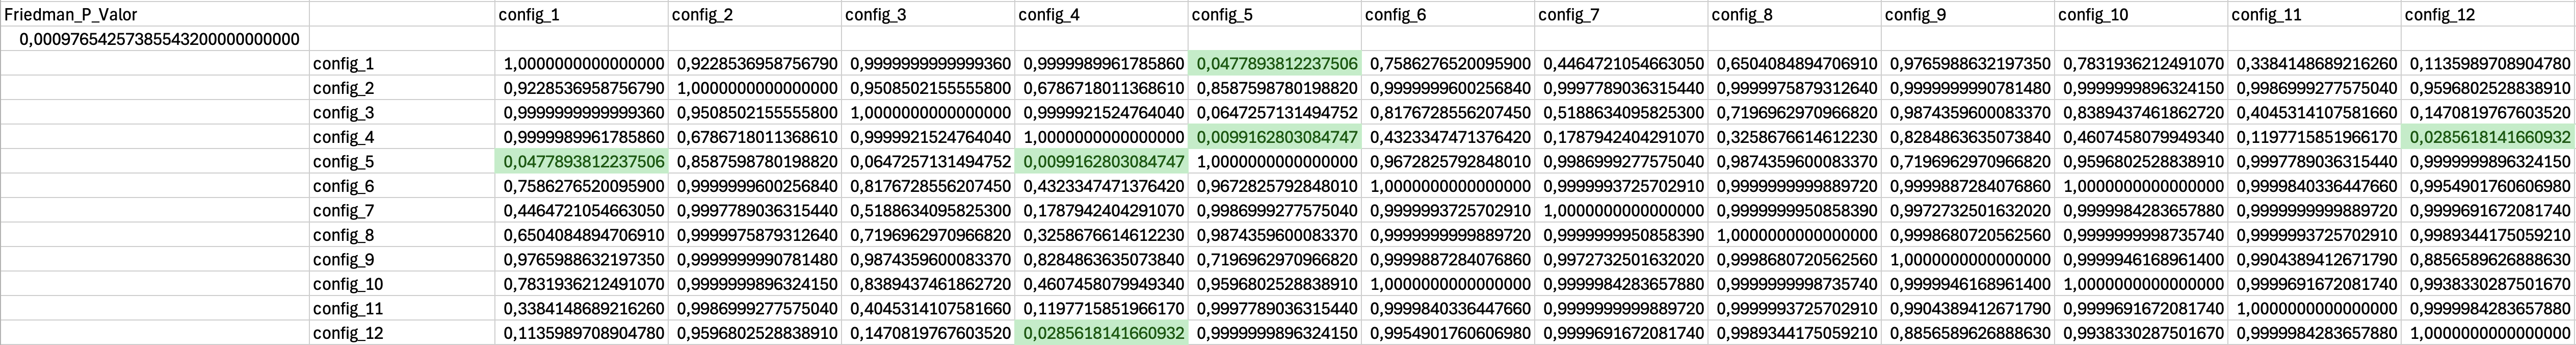
\includegraphics[width=\linewidth,height=\textheight,keepaspectratio]{tabelas/RandomForest-statistic.png}

\vspace{0.5em}
\footnotesize
\textbf{Legenda:} valores-$p$ destacados em verde indicam diferenças estatisticamente significativas (\(p < 0{,}05\)).  
O teste foi aplicado após rejeição da hipótese nula no teste de Friedman.
\end{table}
\end{landscape}


\paragraph{Desempenho Global e Custo Computacional.}
A Figura~\ref{fig:rf-rank} resume o desempenho médio, desvio-padrão e tempo de execução.  
Todos os modelos apresentaram tempos semelhantes ($\approx 1 s$), demonstrando excelente escalabilidade.  
As melhores combinações — \texttt{log\_loss} com 30 ou 100 estimadores — apresentaram desempenho estável, reforçando o equilíbrio entre acurácia e eficiência.

\begin{figure}[H]
\centering
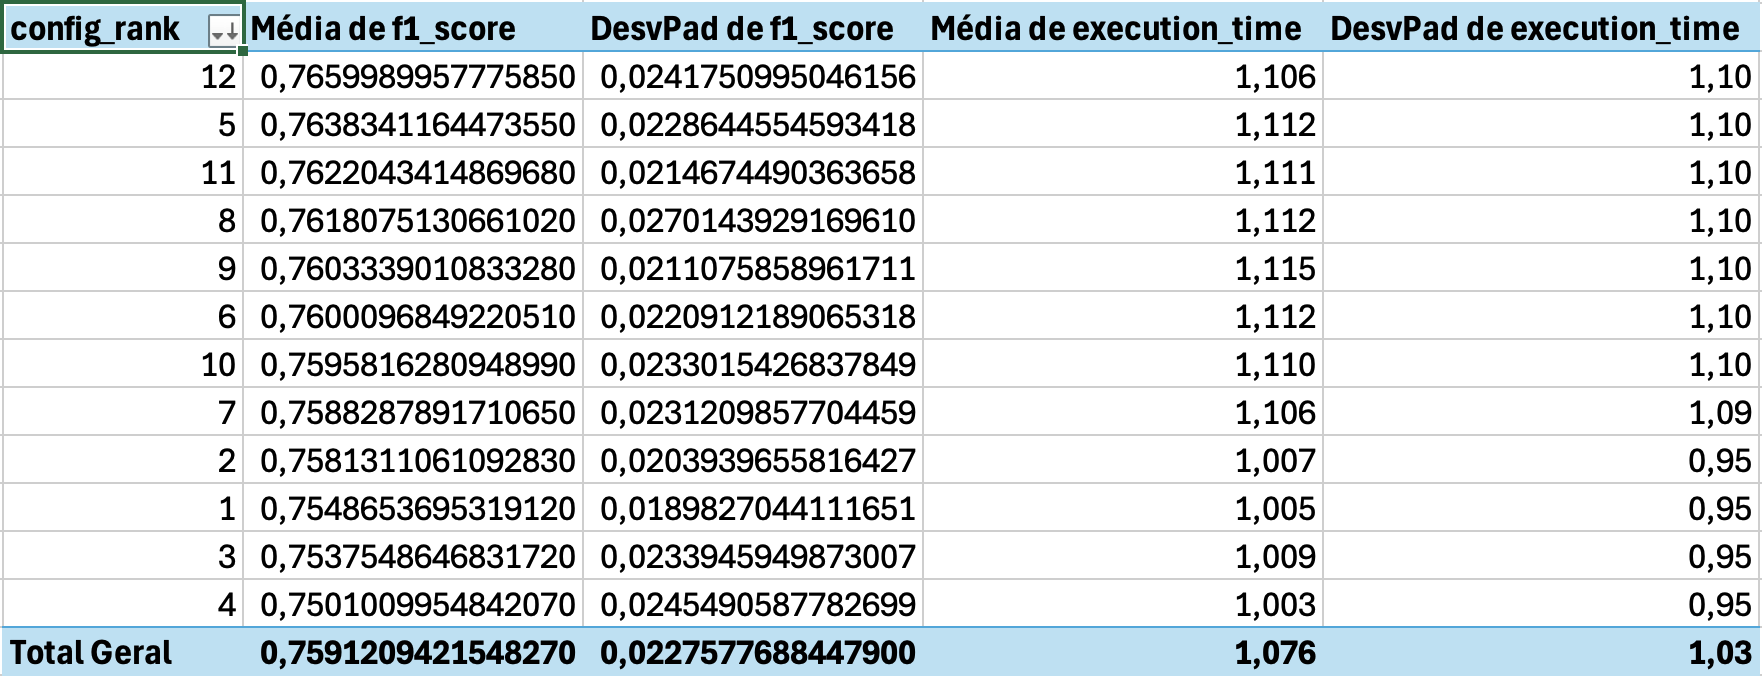
\includegraphics[width=0.9\linewidth]{tabelas/RandomForest-rank.png}
\caption{Desempenho médio, desvio padrão e tempo de execução das doze configurações do Random Forest.}
\label{fig:rf-rank}
\end{figure}


\paragraph{Interpretação dos Resultados.}
O \textit{Random Forest} confirmou o papel do Bagging combinado com aleatorização de atributos como técnica eficaz de redução de variância.  
Os ganhos sobre o \texttt{DecisionTree} individual e sobre o \texttt{Bagging} puro foram consistentes em todas as bases e partições, demonstrando que a diversidade estrutural das árvores é mais determinante que o aumento do número de modelos.  
O método obteve desempenho competitivo próximo ao \texttt{MLP} individual (\(0{,}765\)), com custo computacional significativamente menor e estabilidade superior.

\paragraph{Limitações e Observações.}
Os resultados sugerem que, a partir de 30 árvores, o ganho marginal de desempenho torna-se mínimo, embora o custo de memória continue crescendo linearmente.  
Além disso, as diferenças entre os critérios \texttt{entropy} e \texttt{log\_loss} foram pequenas, indicando que a robustez global do modelo decorre mais da combinação de amostragem e aleatorização do que da escolha da função de impureza.  
De modo geral, o \textit{Random Forest} apresentou comportamento previsível e robusto, consolidando-se como o comitê homogêneo de melhor custo-benefício entre os métodos avaliados.



\subsubsection{Voting}

O método \textit{Voting} foi empregado para combinar classificadores heterogêneos, buscando avaliar o potencial de integração de modelos complementares com diferentes vieses e variâncias.  
Diferentemente dos comitês homogêneos, o Voting opera agregando predições de modelos de naturezas distintas, de forma a aproveitar suas vantagens individuais.  
Foram avaliadas quatro configurações, variando o número de estimadores e a composição entre os modelos base mais bem ranqueados nas seções anteriores.

A Tabela~\ref{tab:voting-config} descreve as configurações avaliadas, considerando que o índice numérico de cada classificador (1 – 6) corresponde à sua posição no ranking das melhores configurações individuais.  
Assim, por exemplo, \texttt{'knn': 1} indica o melhor modelo de KNN, enquanto \texttt{'mlp': 6} representa o sexto colocado entre as configurações de MLP. Os estimadores apresentados são cumulativos. Ou seja, a configuração 2 incorpora todos os estimadores da configuração 1 mais as suas. A configuração 3 incorpora os estimadores das configurações 1 e 2, e assim sucessivamente.

\begin{table}[H]
\centering
\caption{Configurações avaliadas para o comitê heterogêneo Voting.}
\label{tab:voting-config}
\begin{tabularx}{\textwidth}{@{}>{\centering\arraybackslash}p{0.9cm} >{\ttfamily\raggedright\arraybackslash}X@{}}
\toprule
\textbf{Config.} & \textbf{Composição dos classificadores base} \\
\midrule
1 & \{knn: 1, dtree: 1, knn: 6, mlp: 1, mlp: 6\} \\
2 & \{knn: 2, dtree: 2, knn: 8, mlp: 2, dtree: 6\} \\
3 & \{knn: 3, dtree: 3, knn: 7, mlp: 3, dtree: 4\} \\
4 & \{knn: 4, knn: 5, dtree: 5, mlp: 4, mlp: 5\} \\
\bottomrule
\end{tabularx}
\end{table}


\begin{landscape}
\begin{table}[H]
\centering
\caption{Médias de \textit{F1-score} por configuração e base de dados para o comitê Voting.}
\label{tab:voting-matrix}
\vspace{0.5em}

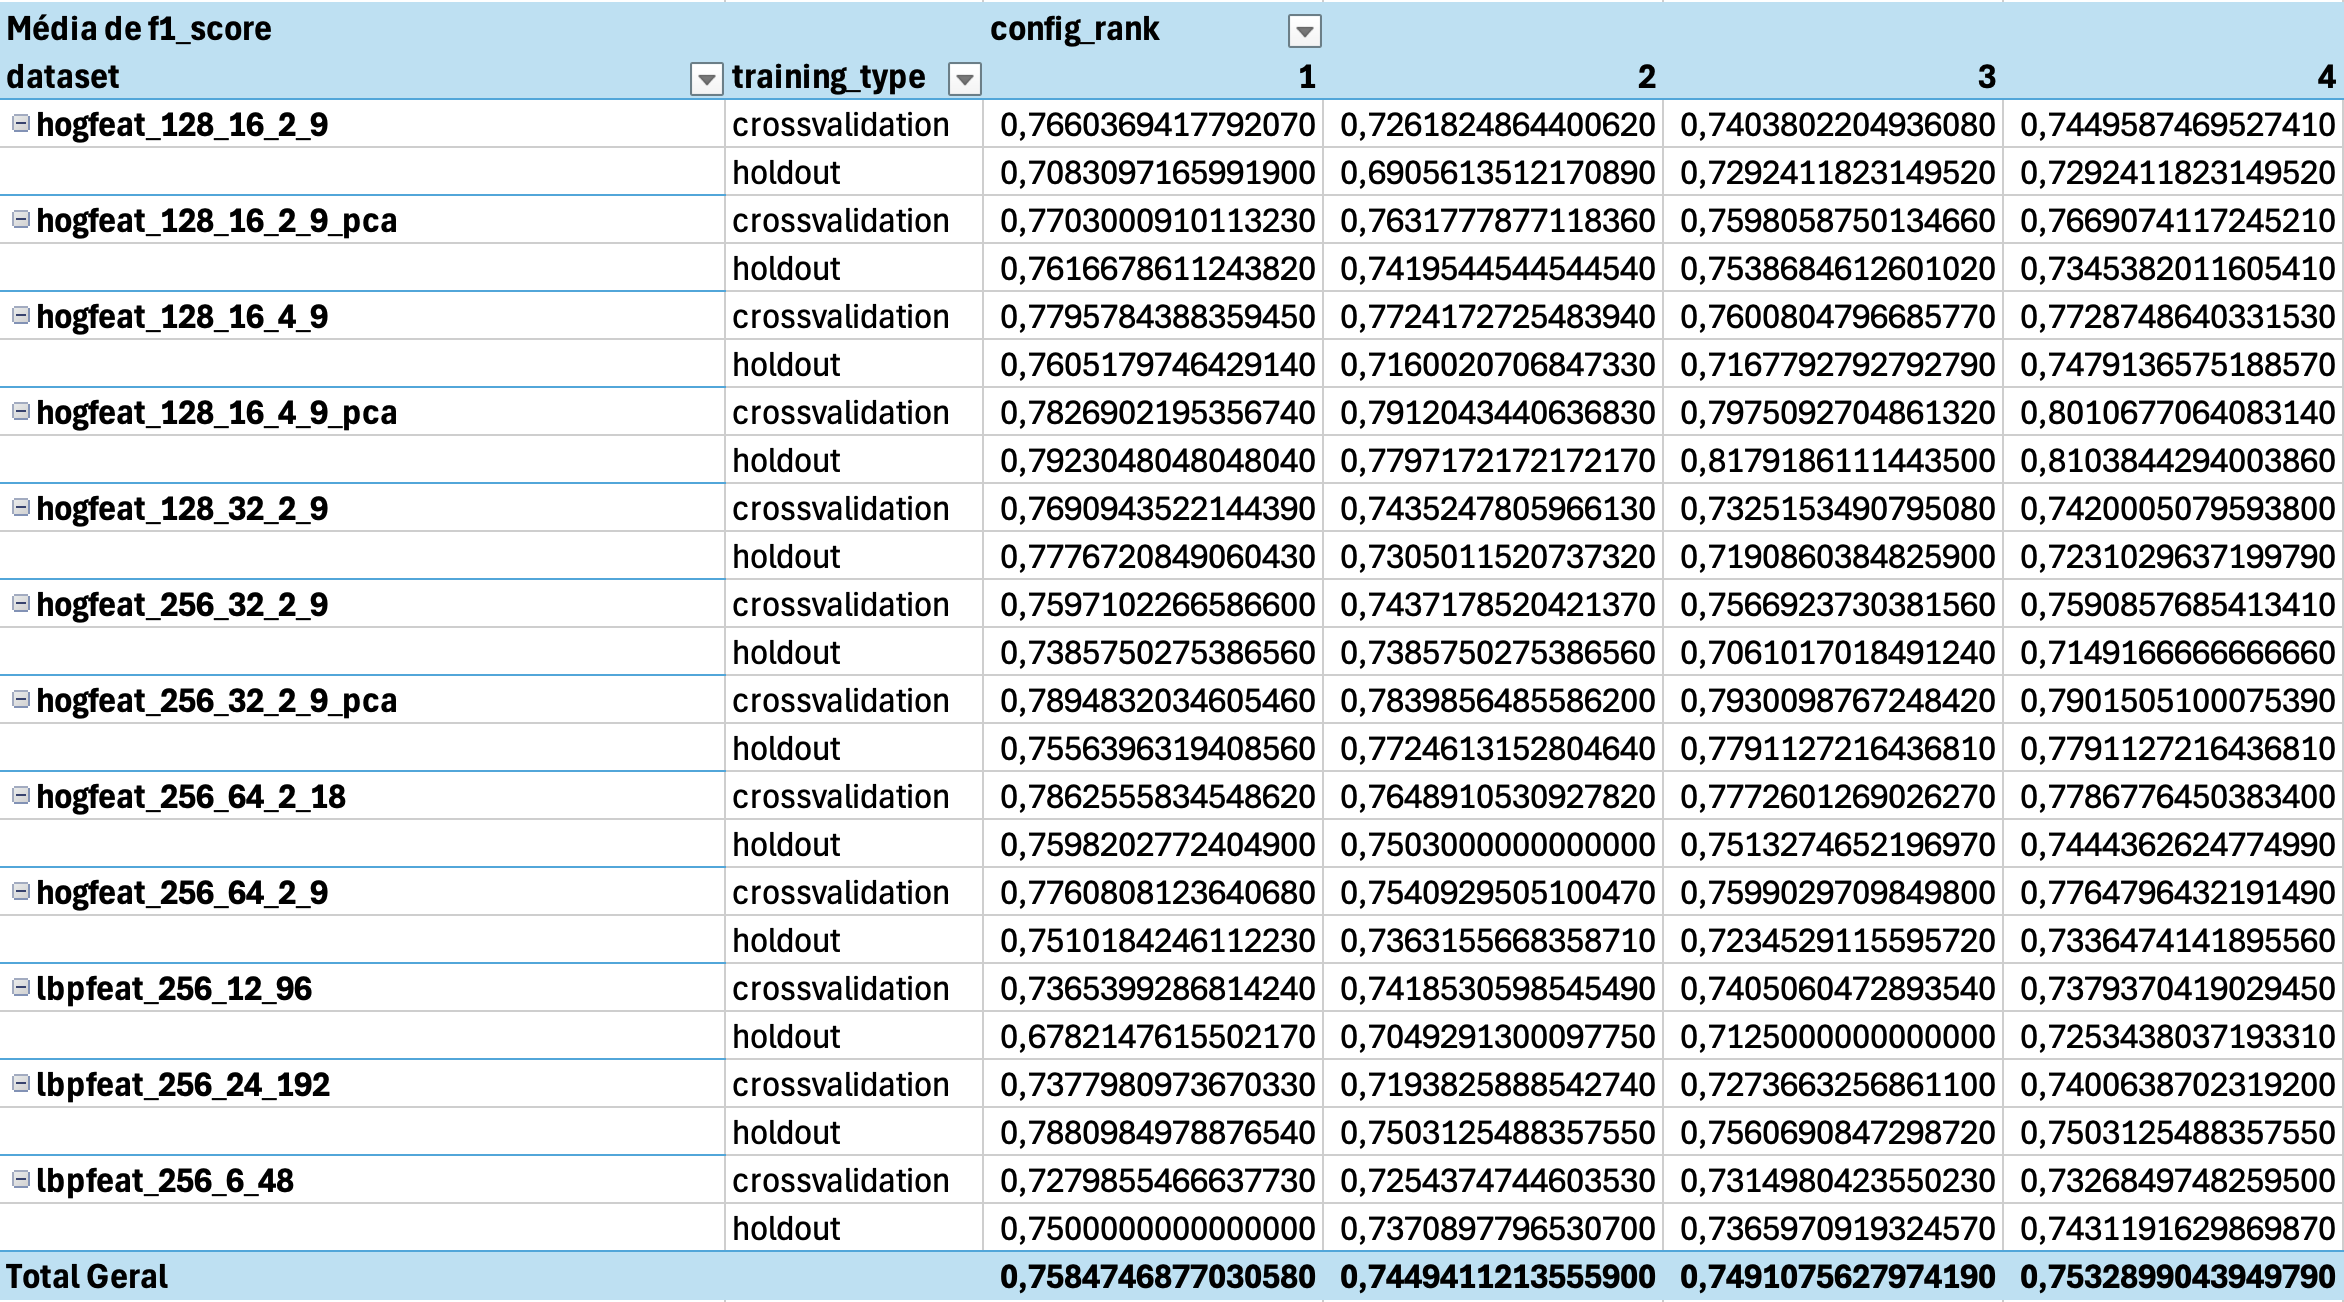
\includegraphics[width=\linewidth,height=\textheight,keepaspectratio]{tabelas/Voting-matrix.png}

\vspace{0.5em}
\footnotesize
\textbf{Legenda:} cada coluna representa uma configuração do comitê heterogêneo, variando a combinação e o número de classificadores participantes.
\end{table}

\vspace{1em}
\normalsize


\paragraph{Comportamento dos Parâmetros.}
A média global de desempenho do Voting foi de \(0{,}751\), situando-se entre os resultados do \texttt{Random Forest} (\(0{,}759\)) e do \texttt{Bagging} (\(0{,}714\)).  
O comitê apresentou desvios-padrão médios em torno de \(0{,}026\), indicando estabilidade moderada entre bases e partições.  
As melhores médias foram obtidas nas configurações 1 e 4 (\(0{,}758\) e \(0{,}753\)), enquanto as demais mantiveram valores próximos, refletindo um comportamento uniforme entre combinações.

O desempenho tendeu a melhorar levemente à medida que o número de estimadores heterogêneos aumentou até cinco modelos, estabilizando-se após esse ponto.  
A inclusão simultânea de \texttt{KNN}, \texttt{DecisionTree} e \texttt{MLP} mostrou-se benéfica, mas os ganhos foram limitados em magnitude — o que sugere que os modelos individuais já cobriam boa parte da diversidade necessária.

Comparando com os classificadores base:
\begin{itemize}
    \item O Voting superou o \texttt{DecisionTree} e o \texttt{KNN} individuais, apresentando ganho médio de \(+0{,}07\) e \(+0{,}14\), respectivamente.
    \item Em relação ao \texttt{Naive Bayes}, o desempenho foi semelhante, dentro da margem de erro experimental.
    \item Frente ao \texttt{MLP}, o Voting apresentou desempenho ligeiramente inferior (\(0{,}751\) vs. \(0{,}765\)), mas com menor variância, indicando maior consistência inter-bases.
\end{itemize}

O custo computacional médio foi de aproximadamente 18 s por execução, compatível com a soma dos tempos médios dos estimadores individuais, refletindo o caráter paralelo e independente do processo de votação.

\end{landscape}


\begin{landscape}
\paragraph{Análise Estatística.}
O teste de Friedman resultou em \( \chi^2_F = 13{,}09 \) e \( p = 0{,}0042 \), indicando diferenças significativas entre as quatro configurações.  
A Tabela~\ref{tab:voting-statistic} apresenta os valores-$p$ do teste de Nemenyi.  
Observa-se que as configurações 1 e 2 diferem significativamente das demais (\(p < 0{,}05\)), representando as combinações mais eficazes entre os modelos heterogêneos.  
A diferença entre as configurações 3 e 4 não foi estatisticamente relevante.

\begin{table}[H]
\centering
\caption{Matriz de comparação par a par do teste de Nemenyi para as quatro configurações do Voting.}
\label{tab:voting-statistic}
\vspace{0.5em}

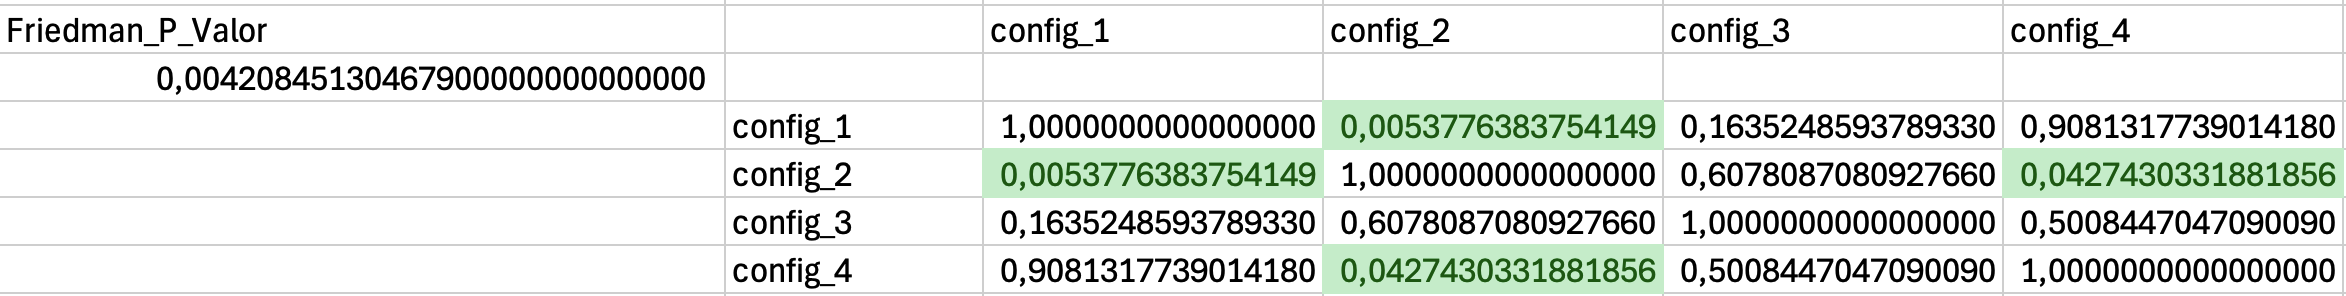
\includegraphics[width=\linewidth,height=\textheight,keepaspectratio]{tabelas/Voting-statistic.png}

\vspace{0.5em}
\footnotesize
\textbf{Legenda:} células destacadas em verde indicam diferenças estatisticamente significativas (\(p < 0{,}05\)).
\end{table}
\end{landscape}


\paragraph{Desempenho Global e Custo Computacional.}
A Figura~\ref{fig:voting-rank} resume o desempenho médio, a dispersão e o tempo de execução das quatro configurações avaliadas.  
Os resultados mostram um equilíbrio entre desempenho e custo: o aumento do número de classificadores ampliou ligeiramente o tempo de execução, mas também reduziu o desvio-padrão e estabilizou o desempenho médio.

\begin{figure}[H]
\centering
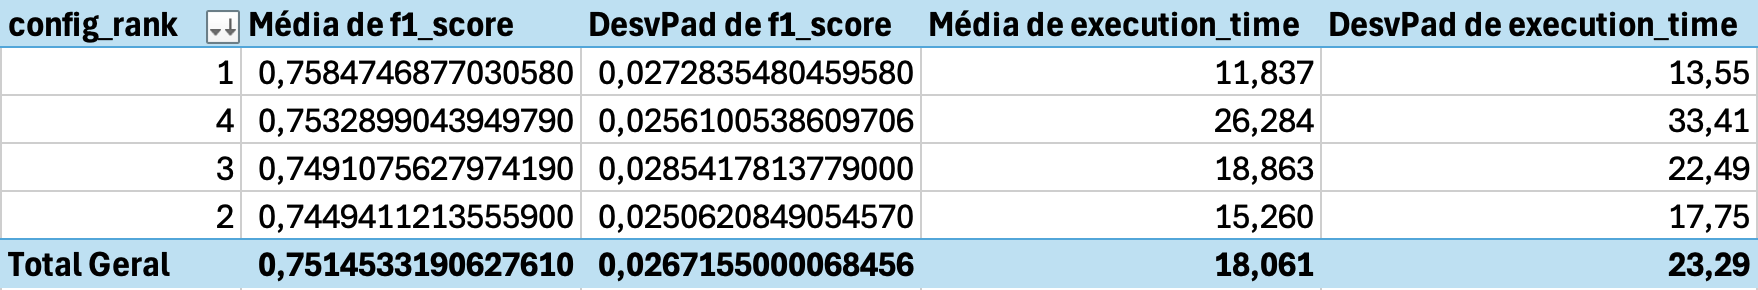
\includegraphics[width=0.9\linewidth]{tabelas/Voting-rank.png}
\caption{Desempenho médio, desvio padrão e tempo de execução das configurações do Voting.}
\label{fig:voting-rank}
\end{figure}


\paragraph{Interpretação dos Resultados.}
Os comitês Voting alcançaram desempenho competitivo com os métodos homogêneos mais robustos.  
Embora não tenham superado o \texttt{Random Forest}, apresentaram relação favorável entre estabilidade e custo computacional.  
O ganho em consistência entre bases distintas demonstra o efeito positivo da heterogeneidade, ainda que limitado pela sobreposição de decisões entre estimadores semelhantes (como múltiplos \texttt{KNN} ou \texttt{MLP}).

\paragraph{Limitações e Observações.}
Os resultados indicam que a estratégia de agregação simples por voto majoritário tem eficácia restrita quando os classificadores apresentam correlações elevadas.  
A diversidade estrutural dos modelos contribuiu para a redução da variância, mas não resultou em ganhos expressivos de \textit{F1-score}.  
Em síntese, o Voting demonstrou bom desempenho médio e estabilidade, mas sua capacidade de generalização depende fortemente da complementaridade efetiva entre os modelos integrantes.

\subsubsection{Stacking}

O método \textit{Stacking} foi avaliado com o objetivo de investigar a eficácia da combinação em múltiplos níveis, na qual as saídas de classificadores base são utilizadas como entradas para um modelo de meta-aprendizado.  
Neste estudo, o \textit{meta-learner} adotado foi uma regressão logística, treinada com predições normalizadas provenientes dos mesmos classificadores heterogêneos empregados no \textit{Voting} (\texttt{KNN}, \texttt{DecisionTree} e \texttt{MLP}).

Foram testadas quatro configurações, idênticas às utilizadas no Voting, variando o número total de estimadores incorporados de forma cumulativa.  
A Tabela~\ref{tab:stacking-config} apresenta as combinações avaliadas.  
Assim, por exemplo, \texttt{'knn': 1} indica o melhor modelo de KNN, enquanto \texttt{'mlp': 6} representa o sexto colocado entre as configurações de MLP.  
Os estimadores são cumulativos: a configuração 2 inclui todos os estimadores da configuração 1 mais as suas; a configuração 3 incorpora os das configurações 1 e 2, e assim por diante.

\begin{table}[H]
\centering
\caption{Configurações avaliadas para o comitê empilhado Stacking.}
\label{tab:stacking-config}
\begin{tabularx}{\textwidth}{@{}>{\centering\arraybackslash}p{0.9cm} >{\ttfamily\raggedright\arraybackslash}X@{}}
\toprule
\textbf{Config.} & \textbf{Composição dos classificadores base} \\
\midrule
1 & \{knn: 1, dtree: 1, knn: 6, mlp: 1, mlp: 6\} \\
2 & \{knn: 2, dtree: 2, knn: 8, mlp: 2, dtree: 6\} \\
3 & \{knn: 3, dtree: 3, knn: 7, mlp: 3, dtree: 4\} \\
4 & \{knn: 4, knn: 5, dtree: 5, mlp: 4, mlp: 5\} \\
\bottomrule
\end{tabularx}
\end{table}


\begin{landscape}
\begin{table}[H]
\centering
\caption{Médias de \textit{F1-score} por configuração e base de dados para o comitê Stacking.}
\label{tab:stacking-matrix}
\vspace{0.5em}

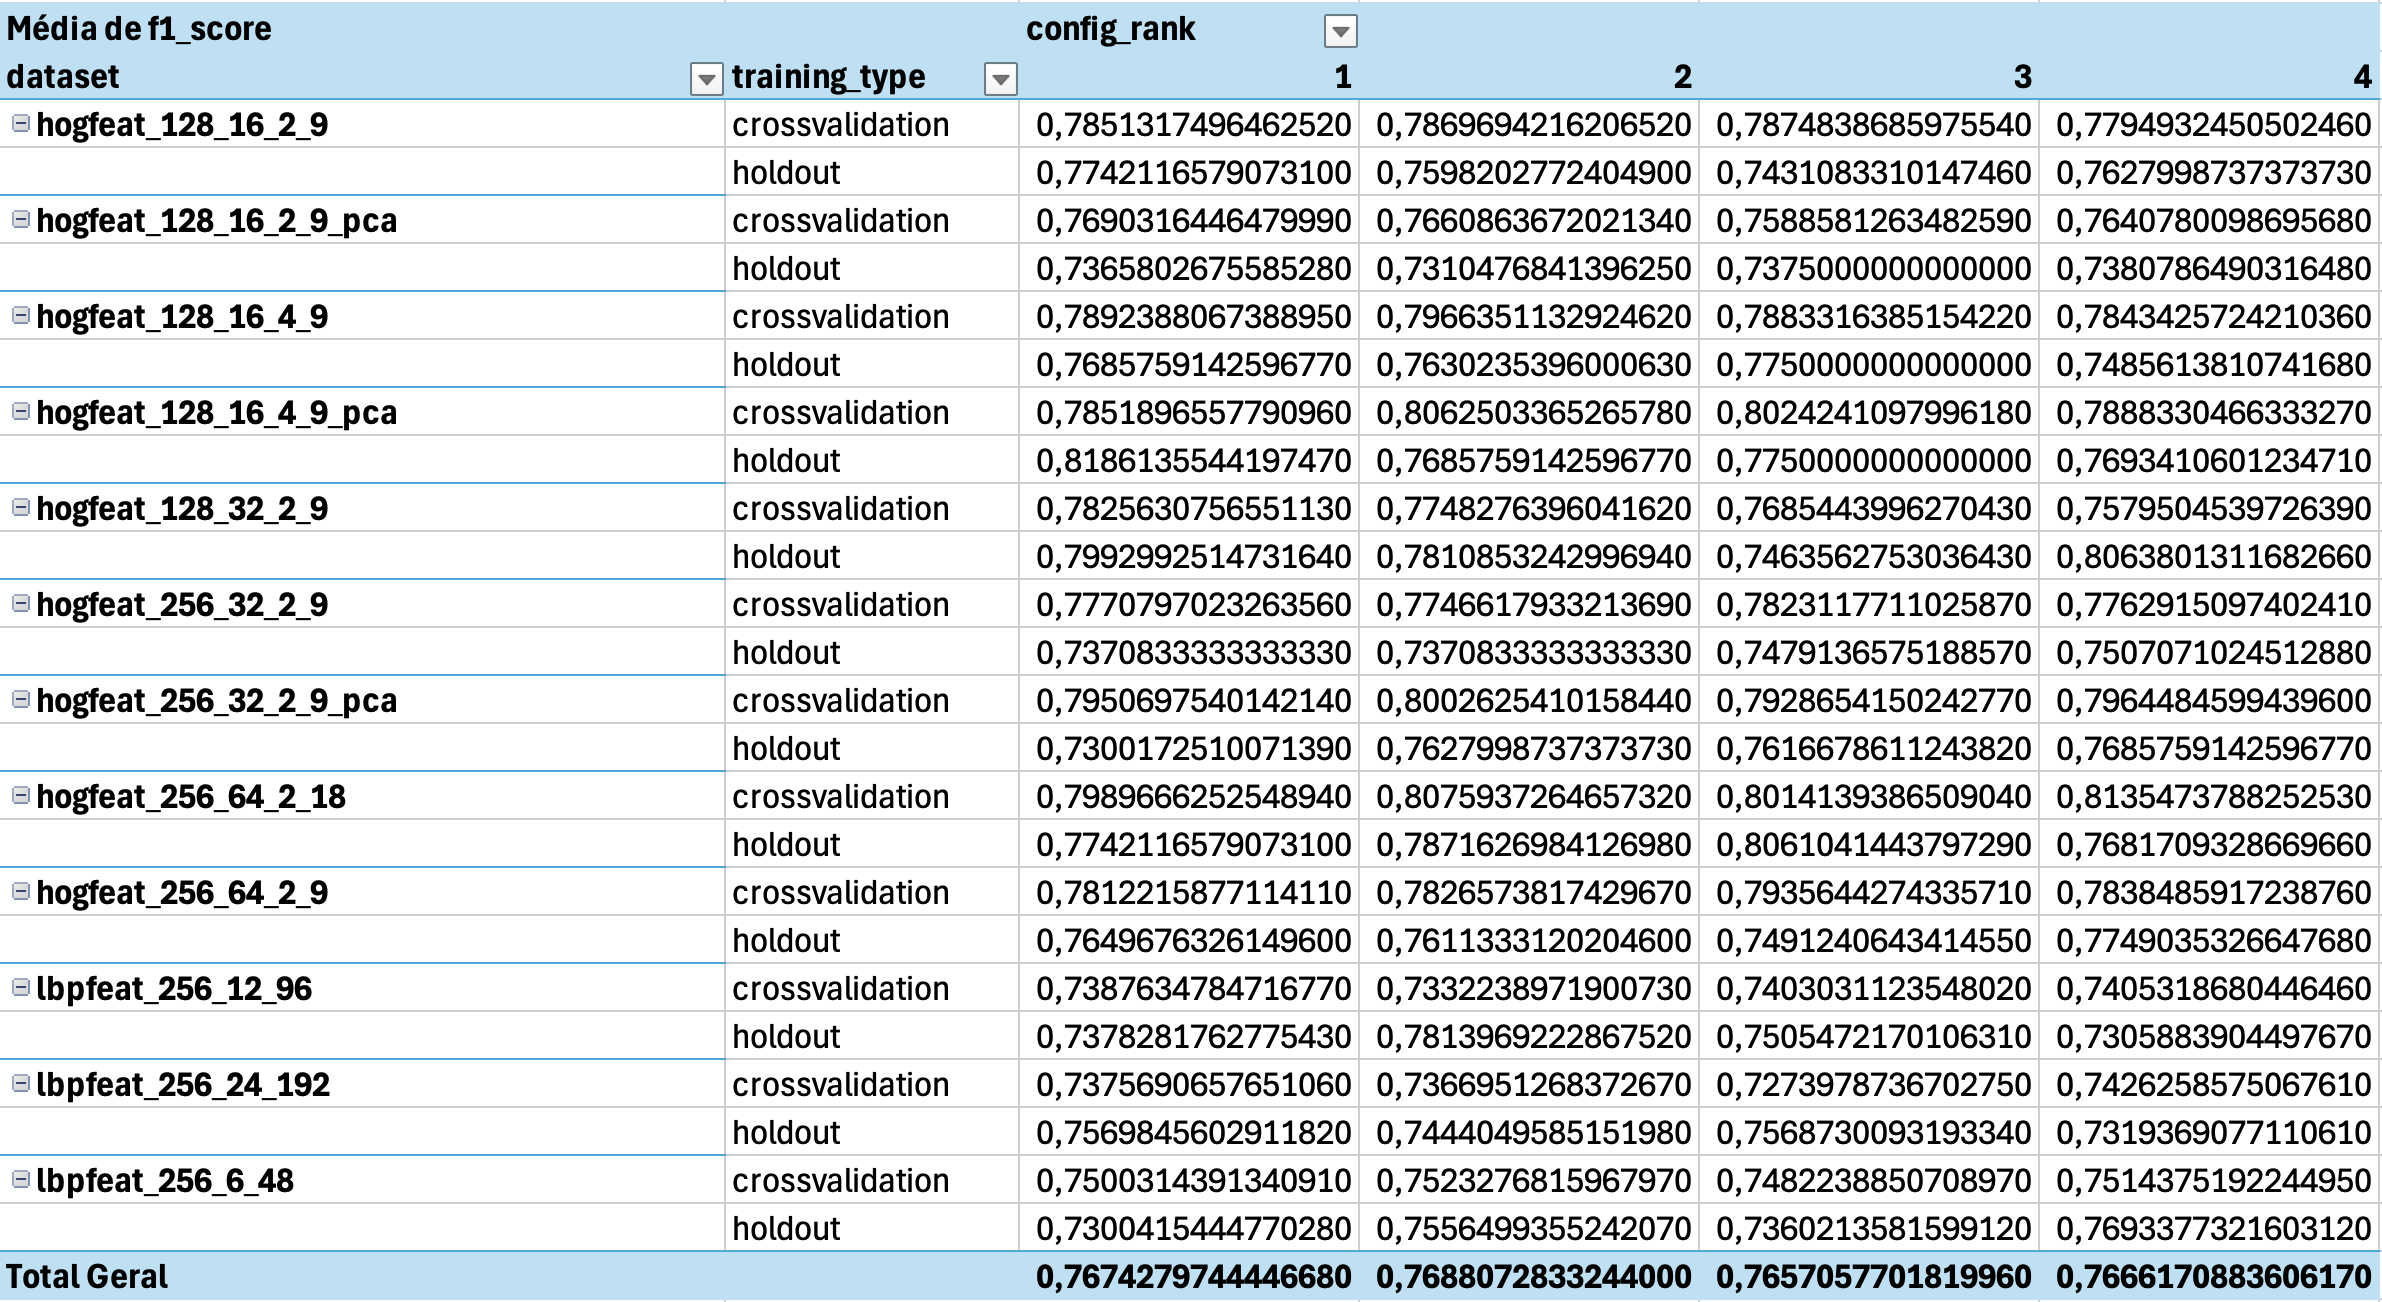
\includegraphics[width=\linewidth,height=\textheight,keepaspectratio]{tabelas/Stacking-matrix.png}

\vspace{0.5em}
\footnotesize
\textbf{Legenda:} cada coluna representa uma configuração do comitê empilhado, variando o número cumulativo de estimadores utilizados como entrada para o meta-aprendiz.
\end{table}

\vspace{1em}
\normalsize


\paragraph{Comportamento dos Parâmetros.}
O \textit{Stacking} apresentou desempenho médio global de \(0{,}767\), o mais alto entre os comitês heterogêneos, com desvio-padrão médio de \(0{,}023\).  
As quatro configurações exibiram resultados muito próximos — variando de \(0{,}765\) a \(0{,}769\) — sem indício de sobreajuste ou degradação com o aumento do número de estimadores.  
Esse comportamento evidencia que o meta-aprendiz foi capaz de integrar adequadamente as saídas dos modelos base, estabilizando o desempenho sem amplificar ruído.

O tempo médio de execução foi de aproximadamente 89 s, com variação acentuada (\(DP = 119\)), reflexo da etapa adicional de treinamento do modelo de nível superior.  
Mesmo assim, o custo manteve-se compatível com o observado nos comitês \texttt{Voting} e \texttt{Random Forest}, preservando boa relação entre desempenho e eficiência.

Comparativamente:
\begin{itemize}
    \item O \texttt{Stacking} superou todos os métodos homogêneos, incluindo o \texttt{Random Forest} (\(+0{,}008\)) e o \texttt{Bagging} (\(+0{,}053\)).
    \item Frente ao \texttt{Voting}, apresentou ganho médio de \(+0{,}016\) pontos de \textit{F1-score}, com menor variância e comportamento mais estável.
    \item Em relação ao \texttt{MLP} individual (\(0{,}765\)), manteve desempenho equivalente, mas com menor dispersão inter-bases, indicando melhor generalização.
\end{itemize}

\end{landscape}


\paragraph{Análise Estatística.}
O teste de Friedman resultou em \( \chi^2_F = 0{,}23 \) e \( p = 0{,}942 \), indicando ausência de diferenças estatisticamente significativas entre as quatro configurações avaliadas.  
Dessa forma, não foi necessária a aplicação do teste de Nemenyi, pois todas as configurações apresentaram desempenho equivalente sob o ponto de vista estatístico.


\paragraph{Desempenho Global e Custo Computacional.}
A Figura~\ref{fig:stacking-rank} resume o desempenho médio, a dispersão e o tempo de execução das quatro configurações avaliadas.  
Os resultados evidenciam alta consistência e estabilidade, com ganhos marginais de desempenho para as configurações intermediárias (2 e 3), sem aumento expressivo no custo computacional.

\begin{figure}[H]
\centering
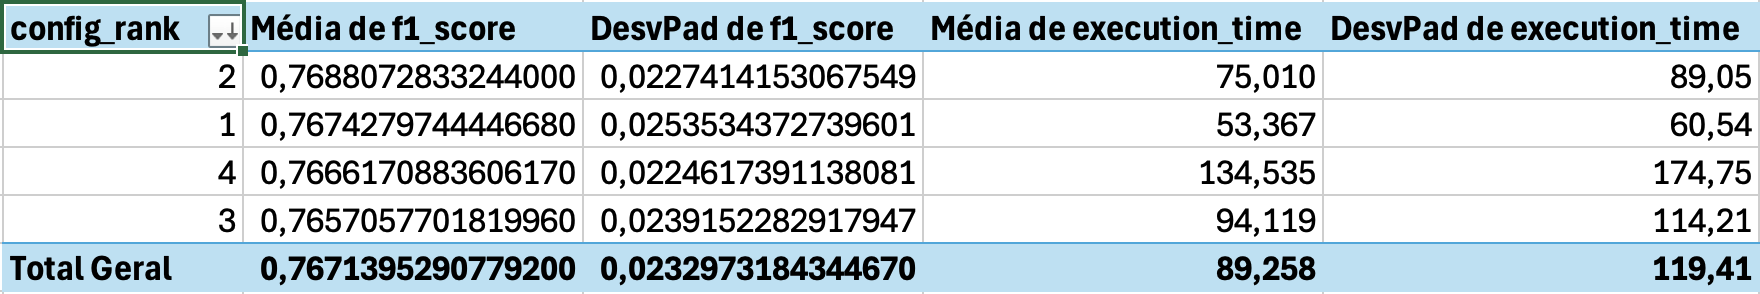
\includegraphics[width=0.9\linewidth]{tabelas/Stacking-rank.png}
\caption{Desempenho médio, desvio padrão e tempo de execução das configurações do Stacking.}
\label{fig:stacking-rank}
\end{figure}


\paragraph{Interpretação dos Resultados.}
Os resultados do Stacking reforçam a hipótese de que o empilhamento supervisionado é capaz de integrar de forma eficiente modelos complementares, aproveitando correlações positivas entre seus erros.  
Embora as diferenças entre as configurações não tenham sido estatisticamente significativas, o método apresentou desempenho consistente e superior aos demais comitês heterogêneos, com estabilidade comparável à do \texttt{MLP} individual.

A ausência de variação relevante entre configurações indica que o meta-aprendiz foi capaz de explorar adequadamente as representações fornecidas pelos classificadores base, atingindo um ponto de saturação informacional já a partir das primeiras combinações.

\paragraph{Limitações e Observações.}
O custo adicional de treinamento e a dependência de um modelo de meta-aprendizado introduzem maior complexidade operacional.  
Ainda assim, o equilíbrio entre acurácia, estabilidade e custo computacional torna o \texttt{Stacking} o comitê mais robusto e consistente entre os métodos avaliados, evidenciando sua capacidade de generalização em contextos heterogêneos.

\subsubsection{Síntese Comparativa entre Comitês}

\paragraph{Análise de Desempenho e Estabilidade.}

A Tabela~\ref{tab:top1-comites-matrix} apresenta o desempenho médio de \textit{F1-score} das melhores configurações de cada comitê — \texttt{Bagging (12)}, \texttt{Random Forest (12)}, \texttt{Voting (1)} e \texttt{Stacking (2)} — sobre os 12 conjuntos de dados experimentais.  
Observa-se que todos os métodos alcançaram médias superiores a \(0{,}75\), com variações reduzidas entre bases, indicando estabilidade e consistência nos resultados.

\begin{landscape}
\begin{table}[H]
\centering
\caption{Desempenho médio (\textit{F1-score}) das melhores configurações de cada comitê.}
\label{tab:top1-comites-matrix}
\vspace{0.5em}
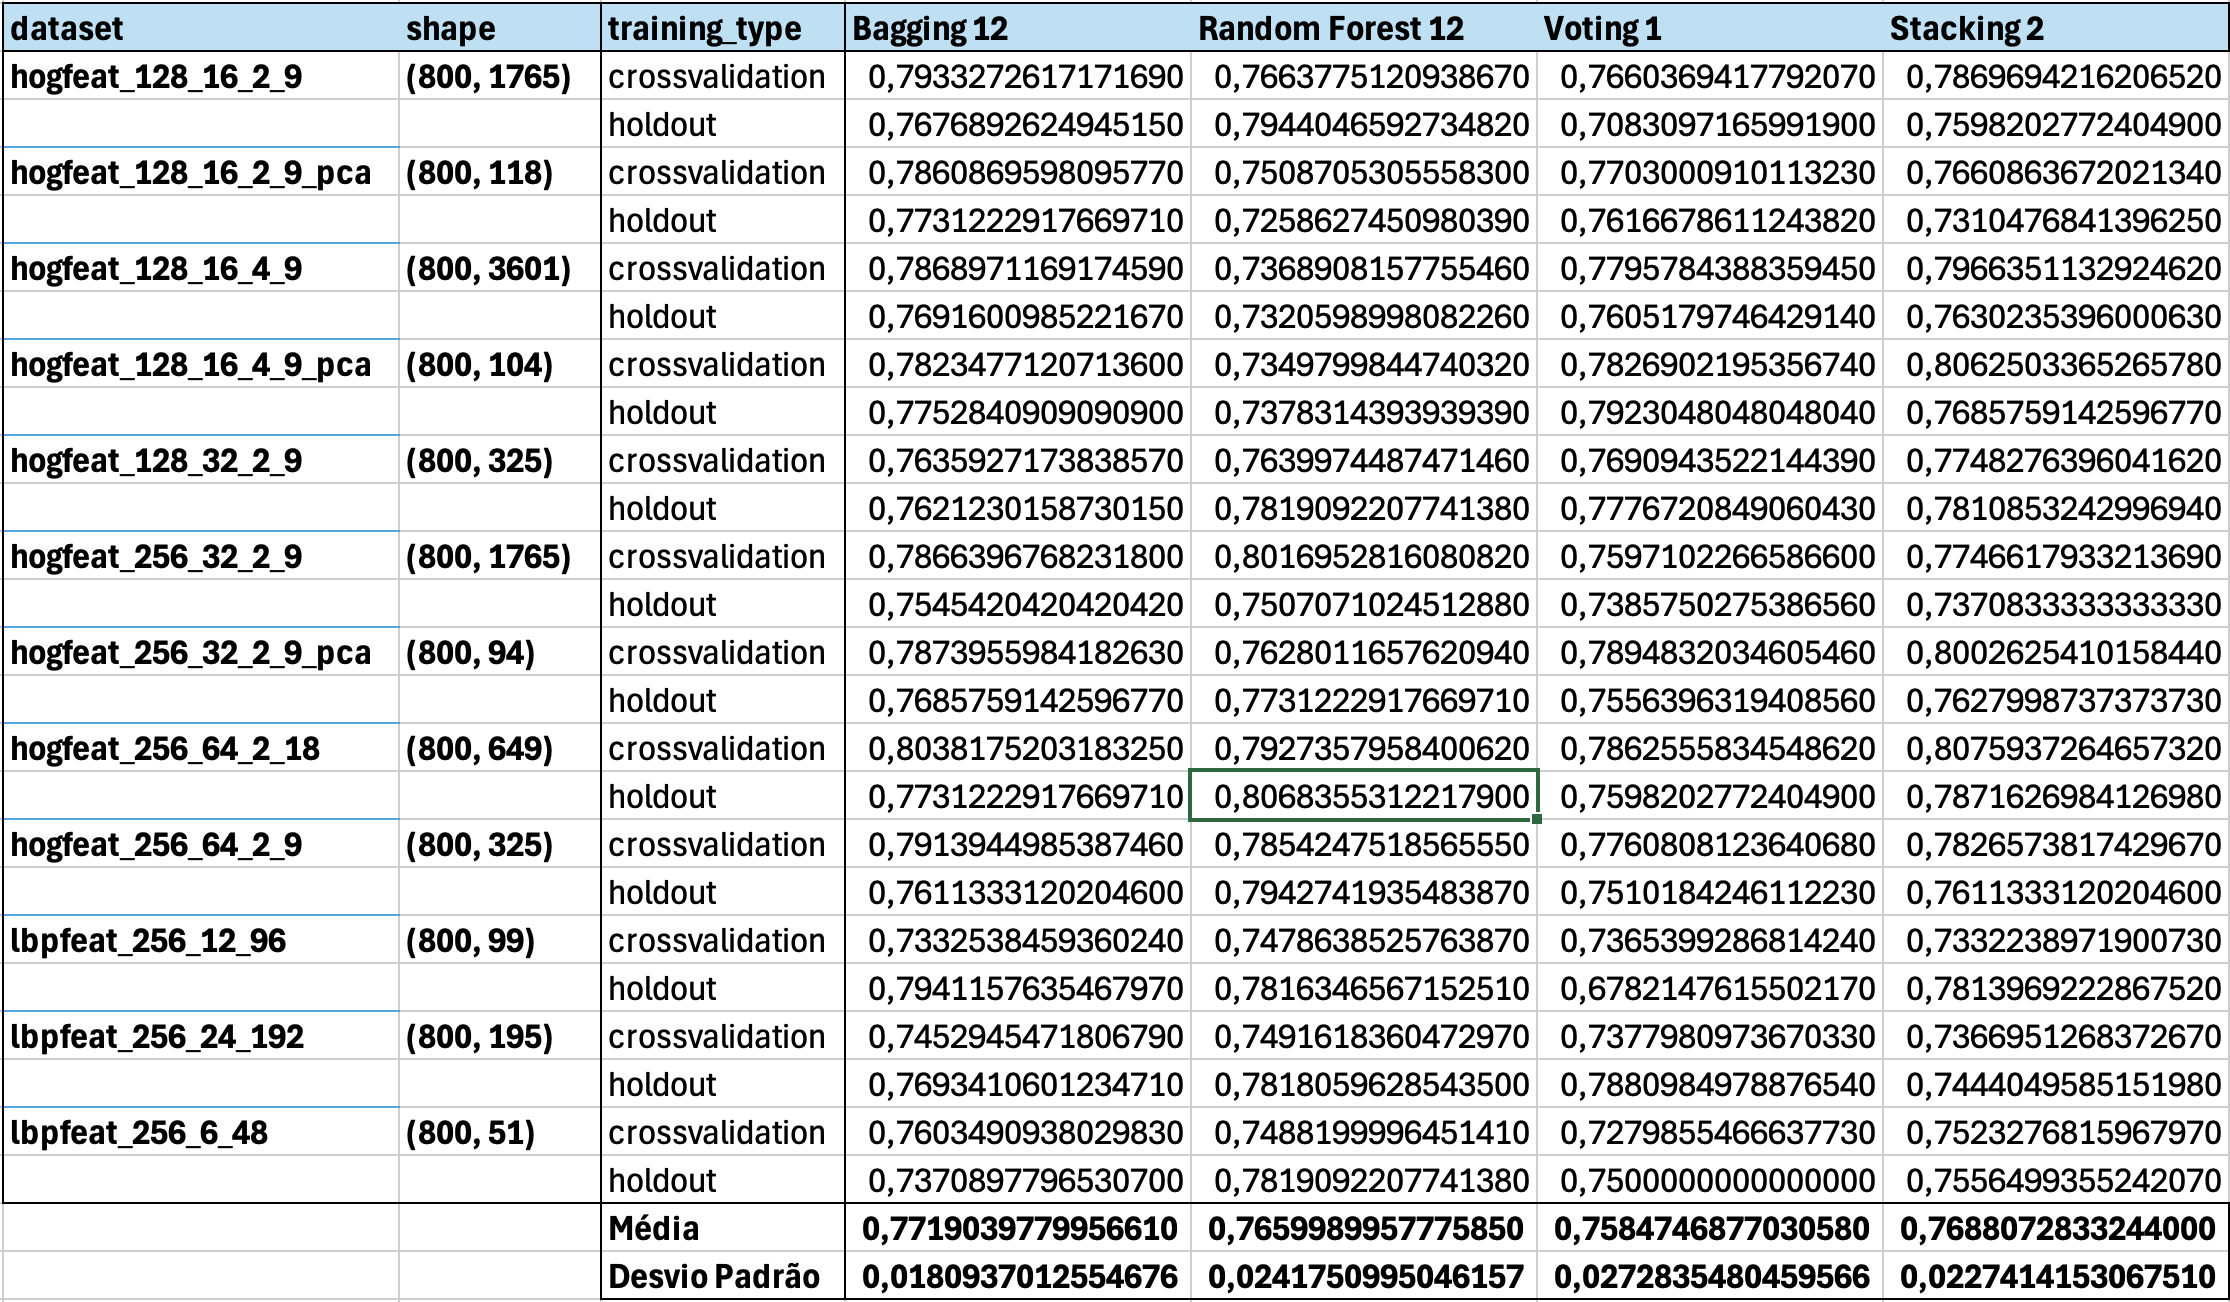
\includegraphics[width=\linewidth,keepaspectratio]{tabelas/top1-comites-matrix.png}
\vspace{0.5em}
\footnotesize
\textbf{Legenda:} cada coluna representa a melhor configuração identificada para cada comitê.  
Os valores correspondem à média de \textit{F1-score} por base, considerando os dois tipos de validação (holdout e crossvalidation).
\end{table}
\end{landscape}

Em termos de desempenho médio global, o \texttt{Bagging} apresentou a maior média de \textit{F1-score} (\(0{,}7719\)), seguido pelo \texttt{Stacking} (\(0{,}7688\)), \texttt{Random Forest} (\(0{,}7659\)) e \texttt{Voting} (\(0{,}7584\)).  
As diferenças numéricas entre os métodos foram pequenas, e os desvios-padrão permaneceram próximos — variando entre \(0{,}018\) e \(0{,}027\) —, o que indica estabilidade dos resultados mesmo diante de variações de descritor, dimensionalidade e iluminação nas imagens.

Na comparação direta, o \texttt{Bagging} apresentou a menor variância e o melhor equilíbrio entre desempenho e robustez, consolidando-se como o comitê mais estável e eficiente em termos médios.  
O \texttt{Random Forest} manteve comportamento intermediário, com desempenho consistente e custo computacional reduzido em relação ao \texttt{Stacking}.  
Por sua vez, o \texttt{Voting} destacou-se pela simplicidade estrutural e pela capacidade de preservar boa performance mesmo com um número reduzido de estimadores, reforçando sua viabilidade em cenários com restrições de recursos.


\paragraph{Resultados dos Testes Estatísticos.}

O teste de Friedman aplicado às médias dos quatro comitês resultou em \( p = 0{,}489 \), não rejeitando a hipótese nula de igualdade de desempenhos.  
Dessa forma, não se observam diferenças estatisticamente significativas entre os métodos quando consideradas suas melhores configurações.  

Esse resultado confirma que, embora o \texttt{Stacking} e o \texttt{Bagging} apresentem médias ligeiramente superiores, tais diferenças não são suficientes para afirmar superioridade estatística sobre os demais.  
Todos os comitês demonstraram desempenho equivalente dentro do intervalo de confiança de 95\%.

\paragraph{Discussão sobre Complexidade e Ganho de Generalização.}

A análise consolidada evidencia que o aumento de complexidade estrutural nem sempre resulta em ganhos expressivos de desempenho.  
O \texttt{Bagging}, embora seja a estrutura mais simples entre os comitês avaliados, apresentou a maior média de \textit{F1-score} e a menor variância, demonstrando que a replicação e agregação de modelos base já são suficientes para alcançar excelente estabilidade e generalização.  
O \texttt{Stacking}, mesmo incorporando um meta-aprendiz adicional, não se mostrou estatisticamente superior, indicando que o ganho obtido não compensa o aumento do custo computacional.

O \texttt{Random Forest} manteve-se como solução intermediária, equilibrando diversidade de estimadores e baixo custo de processamento, enquanto o \texttt{Voting} destacou-se pela simplicidade estrutural e por resultados próximos aos demais, mesmo com combinações lineares de probabilidades.  
Em conjunto, esses achados sugerem que, para conjuntos de dados moderadamente complexos e de tamanho limitado, a diversidade entre classificadores exerce papel mais relevante que a profundidade da combinação.

Assim, todos os comitês avaliados demonstraram potencial de generalização comparável, reforçando que a escolha entre eles deve priorizar o equilíbrio entre custo computacional, estabilidade e finalidade prática da aplicação, e não apenas o ganho marginal em métricas de desempenho.



\subsection{Consolidação dos Resultados e Discussão Final}

\subsubsection{Comparação entre Modelos Individuais e Comitês}

A comparação entre os classificadores individuais e os comitês evidencia que os métodos de agregação tendem a elevar a estabilidade e, em alguns casos, a acurácia dos modelos. Entre os classificadores individuais, o \textit{Multi-Layer Perceptron} (MLP) apresentou o maior desempenho médio (F1 = 0,765), seguido pelo \textit{Naive Bayes} (F1 = 0,737), pela \textit{Árvore de Decisão} (F1 = 0,676) e pelo \textit{k-NN} (F1 = 0,609). Essa diferença, confirmada pelo teste de Friedman ($p < 0{,}001$), demonstrou a superioridade estatisticamente significativa do MLP frente aos demais.

Nos comitês, o desempenho médio global manteve-se elevado e homogêneo entre as técnicas. O \textit{Bagging} apresentou a maior média de F1-score (0,7710), seguido pelo \textit{Stacking} (0,7688), \textit{Random Forest} (0,7659) e \textit{Voting} (0,7584). As diferenças, entretanto, não foram estatisticamente significativas ($p = 0{,}489$), indicando equivalência entre as estruturas. De modo geral, o \textit{Bagging} e o \textit{Random Forest} mostraram melhor relação entre desempenho e custo computacional, enquanto o \textit{Stacking} se destacou pela consistência inter-bases e pelo baixo desvio relativo.

Esses resultados demonstram que, embora os comitês tenham alcançado desempenho ligeiramente superior aos classificadores individuais, o ganho estatístico não foi expressivo. O principal efeito observado foi a redução da variância, consolidando os comitês como abordagens mais estáveis e generalizáveis — com destaque para o \textit{Bagging}, que apresentou o melhor equilíbrio entre desempenho, estabilidade e custo computacional.


\subsubsection{Relação entre Tipo de Descritor e Desempenho}

A análise cruzada dos resultados revela que os descritores HOG produziram sistematicamente melhores desempenhos em relação aos LBP. Essa tendência foi observada tanto nos classificadores individuais quanto nos comitês, refletindo a maior capacidade do HOG em capturar gradientes estruturais relevantes à separação entre cães e gatos. 

As bases reduzidas via PCA apresentaram desempenhos próximos às versões originais, indicando que a compressão preservou a variabilidade essencial dos dados e reduziu o custo de processamento sem perda de acurácia. O efeito do PCA foi particularmente positivo para classificadores sensíveis à dimensionalidade, como o MLP e o Naive Bayes, que mantiveram desempenho elevado mesmo com vetores de características compactos.

Assim, a combinação entre HOG e PCA representou o melhor equilíbrio entre discriminação e eficiência computacional, sendo a base mais robusta para os modelos de maior complexidade.

\subsubsection{Interpretação Estatística Global}

Os testes não paramétricos de Friedman e Nemenyi confirmaram a consistência dos resultados observados. No conjunto dos classificadores individuais, o teste de Friedman ($p < 10^{-10}$) indicou diferenças significativas entre os métodos, e o teste de Nemenyi identificou o MLP como estatisticamente superior aos demais. Já entre os comitês, o teste de Friedman ($p = 0{,}489$) não revelou diferenças estatísticas significativas, o que demonstra equilíbrio de desempenho entre as estruturas \textit{Bagging}, \textit{Random Forest}, \textit{Voting} e \textit{Stacking}.

Esse comportamento reforça a hipótese de que o ganho de desempenho proporcionado pelos comitês decorre principalmente da redução da variância, e não de diferenças intrínsecas entre suas formulações. A homogeneidade dos resultados indica convergência para um limite de desempenho condicionado pelas representações das bases e pela natureza binária do problema.

\subsubsection{Limitações Gerais dos Experimentos}

Entre as limitações observadas, destaca-se o tamanho relativamente reduzido do conjunto de dados (800 imagens), que restringe a capacidade de generalização dos modelos em cenários mais complexos. Além disso, as variações de iluminação e foco, embora representem condições realistas, podem introduzir ruído nas representações de textura, afetando especialmente os descritores LBP. 

O custo computacional dos modelos mais complexos, como o MLP e os comitês baseados nele, também se mostrou elevado, limitando sua aplicabilidade em contextos de restrição de recursos. Por fim, a avaliação concentrou-se na métrica F1-score, sem explorar outras medidas de desempenho que poderiam complementar a análise.

\subsubsection{Síntese Final dos Resultados}

Os resultados consolidados indicam que o MLP individual foi o modelo mais eficiente entre os classificadores básicos, enquanto o \textit{Stacking} apresentou o melhor desempenho médio entre os comitês, embora sem diferença estatística relevante. Os descritores HOG mostraram-se mais discriminativos que os LBP, e o uso do PCA demonstrou ser uma estratégia viável de redução de dimensionalidade.

De modo geral, os comitês proporcionaram ganhos marginais de desempenho e maior estabilidade, confirmando sua eficácia na redução da variância dos modelos. A ausência de diferenças estatísticas significativas entre as estruturas indica que, sob o conjunto de dados utilizado, todas as abordagens convergem para níveis semelhantes de generalização. Esses achados reforçam que a escolha entre modelos deve priorizar o equilíbrio entre custo computacional, estabilidade e interpretabilidade, e não apenas o ganho marginal em métricas de desempenho.


\section{Sugestões para Melhoria dos Experimentos e Dificuldades Encontradas}

Durante a execução dos experimentos, algumas limitações técnicas foram identificadas, especialmente relacionadas à compatibilidade entre as bases reduzidas por PCA e os classificadores probabilísticos da família \textit{Naive Bayes}.  
Após a aplicação do PCA, observou-se a presença de valores negativos nos vetores de características, o que inviabilizou o uso de variantes como o \texttt{MultinomialNB} e o \texttt{ComplementNB}, que exigem atributos estritamente não negativos para o cálculo de probabilidades condicionais.  

Essa restrição também afetou parte dos experimentos envolvendo comitês de classificadores, pois as implementações padrão da biblioteca \texttt{scikit-learn} não permitem aplicar, de forma seletiva, transformações de reescalamento apenas às bases derivadas do PCA dentro de um mesmo pipeline. Consequentemente, em cenários que incluíam classificadores dependentes de entradas positivas, tornou-se impraticável combinar modelos heterogêneos em estruturas como \texttt{Voting} e \texttt{Stacking}.  

Diante desse cenário, optou-se por não utilizar o \textit{Naive Bayes} nas bases em que o PCA gerou valores negativos, a fim de preservar a coerência metodológica e evitar ajustes artificiais de pré-processamento que poderiam introduzir viés. Essa decisão garantiu a comparabilidade entre os experimentos e manteve a integridade estatística das análises.  
Para trabalhos futuros, recomenda-se adotar um controle sistemático sobre a geração de valores negativos durante a redução de dimensionalidade, de modo que a transformação preserve as propriedades numéricas necessárias à aplicação de todos os algoritmos \textit{Naive Bayes}. Esse ajuste deve ser implementado de forma metodológica e uniforme, evitando qualquer desprivilegiamento de classificadores específicos. Alternativamente, pode-se investigar abordagens de normalização adaptativa ou técnicas de PCA não centralizadas, que mantêm a coerência dos dados sem comprometer a distribuição das variáveis.

\paragraph{Desempenho Computacional e Paralelização.}

Outro ponto relevante foi o tempo de execução dos modelos de comitês, particularmente \texttt{Bagging}, \texttt{Random Forest} e \texttt{Stacking}. Mesmo com o uso intensivo de paralelização — utilizando até 12 núcleos de CPU em execução simultânea —, o tempo total permaneceu elevado devido ao grande número de combinações de parâmetros e à complexidade inerente das estruturas de ensemble. Essa limitação reforça a necessidade de estratégias de otimização mais específicas, como redução de busca em grade (\textit{GridSearch}) ou uso de técnicas de amostragem adaptativa de hiperparâmetros.

\paragraph{Dificuldades Específicas no Ajuste do MLP.}

Além disso, observou-se dificuldade particular no ajuste do \texttt{MLPClassifier}. O processo de \textit{GridSearch} enfrentou casos de convergência prematura em determinadas combinações de parâmetros, o que fez com que o número de iterações (\texttt{max\_iter}) influenciasse diretamente a densidade de configurações repetidas entre as dez melhores. Em consequência, diferentes configurações base do modelo apresentaram resultados muito próximos, mas nem sempre representativos do espaço total de busca.  

A alta variabilidade no número de atributos entre as bases também impactou negativamente o processo de ajuste, uma vez que certas arquiteturas de MLP mostraram desempenho superior em conjuntos de baixa dimensionalidade, mas apresentaram queda significativa em bases com maior número de atributos. Diante dessa limitação, foi necessário dividir a busca em dois \textit{GridSearches} menores, adaptados ao porte das bases de entrada. Essa estratégia garantiu convergência estável, mas limitou parcialmente o desempenho global do MLP, já que as configurações selecionadas refletiram um compromisso entre estabilidade e desempenho médio — algumas delas chegando a valores de \textit{F1-score} próximos de 0,80, mas sem consistência entre todas as bases avaliadas.

Por fim, sugere-se ampliar o conjunto de imagens e introduzir novas variações de iluminação e fundo, a fim de reforçar a robustez estatística e a capacidade de generalização dos modelos avaliados, além de investigar arquiteturas paralelas mais eficientes ou soluções baseadas em GPU para reduzir o tempo de processamento dos experimentos futuros.



\section{Conclusão}

Os resultados obtidos neste trabalho permitiram avaliar de forma abrangente o comportamento de diferentes técnicas supervisionadas aplicadas ao problema de classificação binária de imagens de cães e gatos.  
A análise das etapas de pré-processamento, extração de características e aprendizado supervisionado evidenciou a importância do equilíbrio entre representação e complexidade do modelo para alcançar bom desempenho e estabilidade.

Entre os classificadores individuais, o \textit{Multi-Layer Perceptron} (MLP) apresentou o melhor desempenho médio, confirmando sua capacidade de capturar relações não lineares complexas entre os atributos extraídos.  
O \textit{Naive Bayes} destacou-se pela eficiência e desempenho estável em bases sem valores negativos, enquanto a \textit{Árvore de Decisão} e o \textit{k-NN} mostraram comportamento consistente, ainda que mais sensíveis às variações de dimensionalidade e descritor.  
A análise estatística com os testes de Friedman e Nemenyi confirmou a superioridade do MLP entre os modelos individuais de forma estatisticamente significativa.

No conjunto dos comitês de classificadores, observou-se que as estratégias de combinação foram eficazes em reduzir a variância e estabilizar o desempenho entre bases, ainda que com ganhos marginais de acurácia.  
O \texttt{Bagging} apresentou o melhor resultado médio global (\(F1 = 0{,}7719\)), seguido por \texttt{Stacking}, \texttt{Random Forest} e \texttt{Voting}, sem diferenças estatisticamente significativas entre si.  
Esses resultados reforçam que, sob o conjunto de dados e metodologia adotados, o ganho principal das técnicas de ensemble está associado à robustez e à generalização, mais do que ao aumento direto da acurácia média.

Os descritores HOG demonstraram desempenho superior aos LBP, confirmando maior capacidade de representar padrões estruturais relevantes nas imagens.  
O uso do PCA mostrou-se vantajoso como método de redução de dimensionalidade, mantendo desempenho competitivo e reduzindo o custo computacional, ainda que tenha introduzido limitações para o uso pleno dos classificadores probabilísticos.  

As dificuldades encontradas com o \textit{Naive Bayes} e com o processo de \textit{GridSearch} para o MLP reforçaram a importância de uma abordagem metodológica cuidadosa para integração de técnicas com diferentes restrições numéricas e de convergência.  
Essas questões, aliadas à necessidade de paralelização intensiva para execução dos comitês, destacam o desafio de balancear complexidade, desempenho e viabilidade computacional em experimentos supervisionados.

De modo geral, o estudo confirmou que, para conjuntos de dados moderados e com variabilidade controlada, os modelos base bem ajustados podem alcançar desempenho comparável aos comitês mais sofisticados, desde que corretamente parametrizados e avaliados sob protocolos consistentes.  
Os resultados obtidos contribuem para uma compreensão mais clara das relações entre tipo de descritor, estrutura do classificador e estabilidade do aprendizado, oferecendo uma base sólida para estudos futuros envolvendo conjuntos de dados maiores e arquiteturas mais complexas.

Como perspectivas, recomenda-se ampliar o escopo experimental, incluindo métodos de normalização específicos para compatibilizar o PCA com classificadores probabilísticos, além de explorar paralelização em GPU e abordagens de ajuste automatizado de hiperparâmetros.  
Essas melhorias poderão aumentar a eficiência e a generalização dos modelos, fortalecendo o potencial das técnicas supervisionadas aplicadas à classificação de imagens em contextos mais amplos.


\begin{thebibliography}{99}

\bibitem{imd3002-guia}
XAVIER JÚNIOR, João Carlos. \textbf{Guia e materiais da disciplina IMD3002 – Aprendizado de Máquina Supervisionado}.  
Instituto Metrópole Digital, Universidade Federal do Rio Grande do Norte, 2025.  
Disponível nas aulas práticas e teóricas do SIGAA e Google Drive do curso.

\bibitem{imd3002-aulas-praticas}
XAVIER JÚNIOR, João Carlos. \textbf{Materiais de Aula Prática – Técnicas Supervisionadas}.  
IMD3002 – Aprendizado de Máquina Supervisionado, UFRN, 2025.  
Inclui os experimentos com \textit{k-NN}, \textit{Decision Tree}, \textit{Naive Bayes}, \textit{MLP} e Comitês de Classificadores (Bagging, Random Forest, Voting, Stacking).

\bibitem{imd3002-aula25}
XAVIER JÚNIOR, João Carlos. \textbf{Aula 25 – Convolutional Neural Networks (CNN)}.  
IMD3002 – Aprendizado de Máquina Supervisionado, UFRN, 2025.  
Apresentação em slides, Instituto Metrópole Digital.

\bibitem{scikit-learn}
PEDREGOSA, F. et al. \textbf{Scikit-learn: Machine Learning in Python}.  
\textit{Journal of Machine Learning Research}, v. 12, p. 2825–2830, 2011.  
Disponível em: \url{https://scikit-learn.org/stable/}.

\bibitem{dalal-triggs}
DALAL, N.; TRIGGS, B. \textbf{Histograms of Oriented Gradients for Human Detection}.  
In: \textit{Proceedings of the IEEE Conference on Computer Vision and Pattern Recognition (CVPR)}, 2005.

\bibitem{ojala-lbp}
OJALA, T.; PIETIKÄINEN, M.; HARWOOD, D. \textbf{A comparative study of texture measures with classification based on featured distributions}.  
\textit{Pattern Recognition}, v. 29, n. 1, p. 51–59, 1996.

\bibitem{demsar}
DEMSAR, J. \textbf{Statistical comparisons of classifiers over multiple data sets}.  
\textit{Journal of Machine Learning Research}, v. 7, p. 1–30, 2006.

\end{thebibliography}


\end{document}
